% Options for packages loaded elsewhere
\PassOptionsToPackage{unicode}{hyperref}
\PassOptionsToPackage{hyphens}{url}
\PassOptionsToPackage{dvipsnames,svgnames,x11names}{xcolor}
%
\documentclass[
  12pt,
  letterpaper,
  DIV=11,
  numbers=noendperiod]{scrartcl}

\usepackage{amsmath,amssymb}
\usepackage{iftex}
\ifPDFTeX
  \usepackage[T1]{fontenc}
  \usepackage[utf8]{inputenc}
  \usepackage{textcomp} % provide euro and other symbols
\else % if luatex or xetex
  \usepackage{unicode-math}
  \defaultfontfeatures{Scale=MatchLowercase}
  \defaultfontfeatures[\rmfamily]{Ligatures=TeX,Scale=1}
\fi
\usepackage{lmodern}
\ifPDFTeX\else  
    % xetex/luatex font selection
    \setmainfont[]{Times New Roman}
\fi
% Use upquote if available, for straight quotes in verbatim environments
\IfFileExists{upquote.sty}{\usepackage{upquote}}{}
\IfFileExists{microtype.sty}{% use microtype if available
  \usepackage[]{microtype}
  \UseMicrotypeSet[protrusion]{basicmath} % disable protrusion for tt fonts
}{}
\makeatletter
\@ifundefined{KOMAClassName}{% if non-KOMA class
  \IfFileExists{parskip.sty}{%
    \usepackage{parskip}
  }{% else
    \setlength{\parindent}{0pt}
    \setlength{\parskip}{6pt plus 2pt minus 1pt}}
}{% if KOMA class
  \KOMAoptions{parskip=half}}
\makeatother
\usepackage{xcolor}
\setlength{\emergencystretch}{3em} % prevent overfull lines
\setcounter{secnumdepth}{5}
% Make \paragraph and \subparagraph free-standing
\makeatletter
\ifx\paragraph\undefined\else
  \let\oldparagraph\paragraph
  \renewcommand{\paragraph}{
    \@ifstar
      \xxxParagraphStar
      \xxxParagraphNoStar
  }
  \newcommand{\xxxParagraphStar}[1]{\oldparagraph*{#1}\mbox{}}
  \newcommand{\xxxParagraphNoStar}[1]{\oldparagraph{#1}\mbox{}}
\fi
\ifx\subparagraph\undefined\else
  \let\oldsubparagraph\subparagraph
  \renewcommand{\subparagraph}{
    \@ifstar
      \xxxSubParagraphStar
      \xxxSubParagraphNoStar
  }
  \newcommand{\xxxSubParagraphStar}[1]{\oldsubparagraph*{#1}\mbox{}}
  \newcommand{\xxxSubParagraphNoStar}[1]{\oldsubparagraph{#1}\mbox{}}
\fi
\makeatother

\usepackage{color}
\usepackage{fancyvrb}
\newcommand{\VerbBar}{|}
\newcommand{\VERB}{\Verb[commandchars=\\\{\}]}
\DefineVerbatimEnvironment{Highlighting}{Verbatim}{commandchars=\\\{\}}
% Add ',fontsize=\small' for more characters per line
\usepackage{framed}
\definecolor{shadecolor}{RGB}{241,243,245}
\newenvironment{Shaded}{\begin{snugshade}}{\end{snugshade}}
\newcommand{\AlertTok}[1]{\textcolor[rgb]{0.68,0.00,0.00}{#1}}
\newcommand{\AnnotationTok}[1]{\textcolor[rgb]{0.37,0.37,0.37}{#1}}
\newcommand{\AttributeTok}[1]{\textcolor[rgb]{0.40,0.45,0.13}{#1}}
\newcommand{\BaseNTok}[1]{\textcolor[rgb]{0.68,0.00,0.00}{#1}}
\newcommand{\BuiltInTok}[1]{\textcolor[rgb]{0.00,0.23,0.31}{#1}}
\newcommand{\CharTok}[1]{\textcolor[rgb]{0.13,0.47,0.30}{#1}}
\newcommand{\CommentTok}[1]{\textcolor[rgb]{0.37,0.37,0.37}{#1}}
\newcommand{\CommentVarTok}[1]{\textcolor[rgb]{0.37,0.37,0.37}{\textit{#1}}}
\newcommand{\ConstantTok}[1]{\textcolor[rgb]{0.56,0.35,0.01}{#1}}
\newcommand{\ControlFlowTok}[1]{\textcolor[rgb]{0.00,0.23,0.31}{\textbf{#1}}}
\newcommand{\DataTypeTok}[1]{\textcolor[rgb]{0.68,0.00,0.00}{#1}}
\newcommand{\DecValTok}[1]{\textcolor[rgb]{0.68,0.00,0.00}{#1}}
\newcommand{\DocumentationTok}[1]{\textcolor[rgb]{0.37,0.37,0.37}{\textit{#1}}}
\newcommand{\ErrorTok}[1]{\textcolor[rgb]{0.68,0.00,0.00}{#1}}
\newcommand{\ExtensionTok}[1]{\textcolor[rgb]{0.00,0.23,0.31}{#1}}
\newcommand{\FloatTok}[1]{\textcolor[rgb]{0.68,0.00,0.00}{#1}}
\newcommand{\FunctionTok}[1]{\textcolor[rgb]{0.28,0.35,0.67}{#1}}
\newcommand{\ImportTok}[1]{\textcolor[rgb]{0.00,0.46,0.62}{#1}}
\newcommand{\InformationTok}[1]{\textcolor[rgb]{0.37,0.37,0.37}{#1}}
\newcommand{\KeywordTok}[1]{\textcolor[rgb]{0.00,0.23,0.31}{\textbf{#1}}}
\newcommand{\NormalTok}[1]{\textcolor[rgb]{0.00,0.23,0.31}{#1}}
\newcommand{\OperatorTok}[1]{\textcolor[rgb]{0.37,0.37,0.37}{#1}}
\newcommand{\OtherTok}[1]{\textcolor[rgb]{0.00,0.23,0.31}{#1}}
\newcommand{\PreprocessorTok}[1]{\textcolor[rgb]{0.68,0.00,0.00}{#1}}
\newcommand{\RegionMarkerTok}[1]{\textcolor[rgb]{0.00,0.23,0.31}{#1}}
\newcommand{\SpecialCharTok}[1]{\textcolor[rgb]{0.37,0.37,0.37}{#1}}
\newcommand{\SpecialStringTok}[1]{\textcolor[rgb]{0.13,0.47,0.30}{#1}}
\newcommand{\StringTok}[1]{\textcolor[rgb]{0.13,0.47,0.30}{#1}}
\newcommand{\VariableTok}[1]{\textcolor[rgb]{0.07,0.07,0.07}{#1}}
\newcommand{\VerbatimStringTok}[1]{\textcolor[rgb]{0.13,0.47,0.30}{#1}}
\newcommand{\WarningTok}[1]{\textcolor[rgb]{0.37,0.37,0.37}{\textit{#1}}}

\providecommand{\tightlist}{%
  \setlength{\itemsep}{0pt}\setlength{\parskip}{0pt}}\usepackage{longtable,booktabs,array}
\usepackage{calc} % for calculating minipage widths
% Correct order of tables after \paragraph or \subparagraph
\usepackage{etoolbox}
\makeatletter
\patchcmd\longtable{\par}{\if@noskipsec\mbox{}\fi\par}{}{}
\makeatother
% Allow footnotes in longtable head/foot
\IfFileExists{footnotehyper.sty}{\usepackage{footnotehyper}}{\usepackage{footnote}}
\makesavenoteenv{longtable}
\usepackage{graphicx}
\makeatletter
\newsavebox\pandoc@box
\newcommand*\pandocbounded[1]{% scales image to fit in text height/width
  \sbox\pandoc@box{#1}%
  \Gscale@div\@tempa{\textheight}{\dimexpr\ht\pandoc@box+\dp\pandoc@box\relax}%
  \Gscale@div\@tempb{\linewidth}{\wd\pandoc@box}%
  \ifdim\@tempb\p@<\@tempa\p@\let\@tempa\@tempb\fi% select the smaller of both
  \ifdim\@tempa\p@<\p@\scalebox{\@tempa}{\usebox\pandoc@box}%
  \else\usebox{\pandoc@box}%
  \fi%
}
% Set default figure placement to htbp
\def\fps@figure{htbp}
\makeatother
% definitions for citeproc citations
\NewDocumentCommand\citeproctext{}{}
\NewDocumentCommand\citeproc{mm}{%
  \begingroup\def\citeproctext{#2}\cite{#1}\endgroup}
\makeatletter
 % allow citations to break across lines
 \let\@cite@ofmt\@firstofone
 % avoid brackets around text for \cite:
 \def\@biblabel#1{}
 \def\@cite#1#2{{#1\if@tempswa , #2\fi}}
\makeatother
\newlength{\cslhangindent}
\setlength{\cslhangindent}{1.5em}
\newlength{\csllabelwidth}
\setlength{\csllabelwidth}{3em}
\newenvironment{CSLReferences}[2] % #1 hanging-indent, #2 entry-spacing
 {\begin{list}{}{%
  \setlength{\itemindent}{0pt}
  \setlength{\leftmargin}{0pt}
  \setlength{\parsep}{0pt}
  % turn on hanging indent if param 1 is 1
  \ifodd #1
   \setlength{\leftmargin}{\cslhangindent}
   \setlength{\itemindent}{-1\cslhangindent}
  \fi
  % set entry spacing
  \setlength{\itemsep}{#2\baselineskip}}}
 {\end{list}}
\usepackage{calc}
\newcommand{\CSLBlock}[1]{\hfill\break\parbox[t]{\linewidth}{\strut\ignorespaces#1\strut}}
\newcommand{\CSLLeftMargin}[1]{\parbox[t]{\csllabelwidth}{\strut#1\strut}}
\newcommand{\CSLRightInline}[1]{\parbox[t]{\linewidth - \csllabelwidth}{\strut#1\strut}}
\newcommand{\CSLIndent}[1]{\hspace{\cslhangindent}#1}

\usepackage{tcolorbox}
\usepackage{amssymb}
\usepackage{yfonts}
\usepackage{bm}


\newtcolorbox{greybox}{
  colback=white,
  colframe=blue,
  coltext=black,
  boxsep=5pt,
  arc=4pt}
  
 
\newcommand{\ds}[4]{\sum_{{#1}=1}^{#3}\sum_{{#2}=1}^{#4}}
\newcommand{\us}[3]{\mathop{\sum\sum}_{1\leq{#2}<{#1}\leq{#3}}}

\newcommand{\ol}[1]{\overline{#1}}
\newcommand{\ul}[1]{\underline{#1}}

\newcommand{\amin}[1]{\mathop{\text{argmin}}_{#1}}
\newcommand{\amax}[1]{\mathop{\text{argmax}}_{#1}}

\newcommand{\ci}{\perp\!\!\!\perp}

\newcommand{\mc}[1]{\mathcal{#1}}
\newcommand{\mb}[1]{\mathbb{#1}}
\newcommand{\mf}[1]{\mathfrak{#1}}

\newcommand{\eps}{\epsilon}
\newcommand{\lbd}{\lambda}
\newcommand{\alp}{\alpha}
\newcommand{\df}{=:}
\newcommand{\am}[1]{\mathop{\text{argmin}}_{#1}}
\newcommand{\ls}[2]{\mathop{\sum\sum}_{#1}^{#2}}
\newcommand{\ijs}{\mathop{\sum\sum}_{1\leq i<j\leq n}}
\newcommand{\jis}{\mathop{\sum\sum}_{1\leq j<i\leq n}}
\newcommand{\sij}{\sum_{i=1}^n\sum_{j=1}^n}

\newcommand{\sectionbreak}{\pagebreak}


	
\KOMAoption{captions}{tableheading}
\makeatletter
\@ifpackageloaded{caption}{}{\usepackage{caption}}
\AtBeginDocument{%
\ifdefined\contentsname
  \renewcommand*\contentsname{Table of contents}
\else
  \newcommand\contentsname{Table of contents}
\fi
\ifdefined\listfigurename
  \renewcommand*\listfigurename{List of Figures}
\else
  \newcommand\listfigurename{List of Figures}
\fi
\ifdefined\listtablename
  \renewcommand*\listtablename{List of Tables}
\else
  \newcommand\listtablename{List of Tables}
\fi
\ifdefined\figurename
  \renewcommand*\figurename{Figure}
\else
  \newcommand\figurename{Figure}
\fi
\ifdefined\tablename
  \renewcommand*\tablename{Table}
\else
  \newcommand\tablename{Table}
\fi
}
\@ifpackageloaded{float}{}{\usepackage{float}}
\floatstyle{ruled}
\@ifundefined{c@chapter}{\newfloat{codelisting}{h}{lop}}{\newfloat{codelisting}{h}{lop}[chapter]}
\floatname{codelisting}{Listing}
\newcommand*\listoflistings{\listof{codelisting}{List of Listings}}
\usepackage{amsthm}
\theoremstyle{definition}
\newtheorem{definition}{Definition}[section]
\theoremstyle{plain}
\newtheorem{theorem}{Theorem}[section]
\theoremstyle{plain}
\newtheorem{lemma}{Lemma}[section]
\theoremstyle{remark}
\AtBeginDocument{\renewcommand*{\proofname}{Proof}}
\newtheorem*{remark}{Remark}
\newtheorem*{solution}{Solution}
\newtheorem{refremark}{Remark}[section]
\newtheorem{refsolution}{Solution}[section]
\makeatother
\makeatletter
\makeatother
\makeatletter
\@ifpackageloaded{caption}{}{\usepackage{caption}}
\@ifpackageloaded{subcaption}{}{\usepackage{subcaption}}
\makeatother

\usepackage{bookmark}

\IfFileExists{xurl.sty}{\usepackage{xurl}}{} % add URL line breaks if available
\urlstyle{same} % disable monospaced font for URLs
\hypersetup{
  pdftitle={Robust Least Squares Multidimensional Scaling},
  pdfauthor={Jan de Leeuw},
  colorlinks=true,
  linkcolor={blue},
  filecolor={Maroon},
  citecolor={Blue},
  urlcolor={Blue},
  pdfcreator={LaTeX via pandoc}}


\title{Robust Least Squares Multidimensional Scaling}
\author{Jan de Leeuw}
\date{October 18, 2024}

\begin{document}
\maketitle
\begin{abstract}
Combining different loss functions with linear models and minimizing
loss with iteratively reweighted least squares (IRLS) has a long history
in robust statistics. In this paper we use an IRLS version of the smacof
algorithm to minimize various robust multidimensional scaling loss
functions. Our results use a general theorem on sharp quadratic
majorization of De Leeuw and Lange
(\citeproc{ref-deleeuw_lange_A_09}{2009}). We relate this theorem to
earlier results in robust statistics, location theory, and sparse
recovery. Code in R is included.
\end{abstract}

\renewcommand*\contentsname{Table of contents}
{
\hypersetup{linkcolor=}
\setcounter{tocdepth}{3}
\tableofcontents
}

\sectionbreak

\listoffigures

\sectionbreak

\section{Introduction}\label{introduction}

The title of this paper is somewhat paradoxical. Least squares
estimation is typically not robust, it is sensitive to outliers and pays
too much attention to minimizing the largest residuals. What we mean by
robust least squares multidimensional scaling (MDS), however, is using
the smacof machinery designed to minimize least squares loss functions
of the form \begin{equation}
\sigma_2(X):=\sum \omega_k(\delta_k-d_k(X))^2\label{eq:stressdef},
\end{equation} to minimize robust loss functions.

The prototypical robust loss function is least absolute value loss
\begin{equation}
\sigma_1(X):=\sum \omega_k|\delta_k-d_k(X)|\label{eq:stradddef},
\end{equation} which we will call \emph{strife}, because the names
\emph{stress}, \emph{sstress}, and \emph{strain} are already taken.

Strife is not differentiable at configurations \(X\) for which there is
at least one \(k\) for which either \(d_k(X)=\delta_k\) or \(d_k(X)=0\)
(or both). This lack of differentiability complicates the minimization
problem. Moreover experience with one-dimensional and city block MDS
suggests that having areas where the loss function is not differentiable
leads to (many) additional local minima.

In this paper we will discuss (and implement) various variations of
\(\sigma_1\) from \eqref{eq:stradddef}. They can be interpreted in two
different ways. On the one hand we use smoothers of the absolute value
function, and consequently of strife. We want to eliminate the problems
with differentiability, at least the ones caused by \(\delta_k=d_k(X)\).
If this is our main goal, then we want to choose the smoother in such a
way that it is close to the absolute value function. This is not unlike
the distance smoothing used by Pliner (\citeproc{ref-pliner_96}{1996})
and Groenen, Heiser, and Meulman
(\citeproc{ref-groenen_heiser_meulman_99}{1999}) in the global
minimization of \(\sigma_2\) from \eqref{eq:stressdef}.

On the other hand our modified loss function can be interpreted as more
robust versions of the least squares loss function, and consequently of
stress. Our goal then is to combines the robustness of the absolute
value function with the efficiency and computational ease of least
squares. If robustness is our goal then there is no reason to stay that
close to the absolute value function.

Our robust or smooth loss functions are all of the form \begin{equation}
\sigma(X):=\sum \omega_k\ f_c(\delta_k-d_k(X))\label{eq:strifedef},
\end{equation} for a suitable choice of the real valued function \(f\).
We will define what we mean by ``suitable'' later on. The subscript
\(c\) of \(f_c\) is meant to indicate that the loss function may depend
on one or more real-valued tuning parameters \(c\) that regulate the
degree of smoothness and/or robustness. For now, note that loss
\eqref{eq:stressdef} is the special case with \(f_c(x)=x^2\) and loss
\eqref{eq:stradddef}is the special case with \(f_c(x)=|x|\). There is no
tuning in both these cases.

\sectionbreak

\section{Majorizing Strife}\label{sec-majorization}

The idea of minimizing a least absolute value (LAV) to obtain parameter
estimates dates back to the work of Boskovitch in the middle of the
eighteenth century. Until recently it has been applied mainly to fit
linear models, so that we can actually use standard linear programming
algorithms to obtain optimal solutions.

The pioneering work in MDS strife minimization using smacof is Heiser
(\citeproc{ref-heiser_88}{1988}), which builds on earlier work of Heiser
(\citeproc{ref-heiser_87}{1987}). It is based on a creative use of the
Arithmetic Mean-Geometric Mean (AM/GM) inequality to find a majorizer of
the absolute value function. For the general theory of majorization
algorithms (now more commonly known as MM algorithms) we refer to their
original introduction in De Leeuw (\citeproc{ref-deleeuw_C_94c}{1994})
and to the excellent recent book by Lange
(\citeproc{ref-lange_16}{2016}).

The AM/GM inequality says that for all non-negative \(x\) and \(y\) we
have \begin{equation}
|x||y|=\sqrt{x^2y^2}\leq\frac12(x^2+y^2),\label{eq:amgm}
\end{equation} with equality if and only if \(x^2=y^2\). If \(y>0\) we
can write \eqref{eq:amgm} as \begin{equation}
|x|\leq\frac12\frac{1}{|y|}(x^2+y^2),\label{eq:amgmmaj}
\end{equation} and this provides a quadratic majorization of \(|x|\) at
\(y\). There is no quadratic majorization of \(|x|\) at \(y=0\), which
is a problem we will have to deal with.

Using the majorization \eqref{eq:amgmmaj}, and assuming
\(\delta_k\not=d_k(Y)\) for all \(k\), we define \begin{equation}
\omega_1(X):=\frac12\sum \omega_k\frac{1}{|\delta_k-d_k(Y)|}((\delta_k-d_k(Y))^2+(\delta_k-d_k(X))^2).\label{eq:omegadef}
\end{equation} Now \(\sigma_1(X)\leq\omega_1(X)\) for all \(X\) and
\(\sigma_1(Y)=\omega_1(Y)\), and thus \(\omega_1\) majorizes
\(\sigma_1\) at \(Y\).

\subsection{Algorithm}\label{sec-amgm}

Define \begin{equation}
\omega_k(Y):=\omega_k\frac{1}{|\delta_k-d_k(Y)|}.\label{eq:wk1def}
\end{equation} Reweighted smacof to minimize strife computes
\(X^{(k+1)}\) by decreasing \begin{equation}
\sum \omega_k(X^{(k)})(\delta_k-d_k(X^{(k)}))^2,\label{eq:sstrf}
\end{equation} using a standard smacof step. It then computes the new
weights \(\omega_k(X^{(k+1)})\) from \eqref{eq:wk1def} and uses them in
the next smacof step to update \(X^{(k+1)}\). And so on, until
convergence.

A straightforward variation of the algorithm does a number of smacof
steps before upgrading the weights. This still leads to a monotone, and
thus convergent, algorithm. How many smacof steps we have to take in the
inner iterations is something that needs further study. It is likely to
depend on the fit of the data, on the shape of the function near the
local minimum, and on how far the iterations are from the local minimum.

\subsection{Zero Residuals}\label{sec-zero}

It may happen that for some \(k\) we have \(d_k(X^{(k)})=\delta_k\)
while iterating. There have been various proposals to deal with such an
unfortunate event, and we will discuss some of them further on. Even
more importantly we will see that that the minimizer of the absolute
value loss usually satisfies \(d_k(X)=\delta_k\) for quite a few
elements, which means that near convergence the algorithm will become
unstable because the weights from \eqref{eq:wk1def} become very large.

A large number of somewhat ad-hoc solutions have been proposed to deal
with the problem of zero residuals, both in location analysis and in the
statistical literature. We tend to agree with the assessment of Aftab
and Hartley (\citeproc{ref-aftab_hartley_15}{2015}).

\begin{quote}
.. attempts to analyze this difficulty {[}caused by infinite weights of
IRLS for the \(\ell_p\)-loss{]} have a long history of proofs and
counterexamples to incorrect claims.
\end{quote}

Schlossmacher (\citeproc{ref-schlossmacher_73}{1973}) is the first
discussion of the majorization method in the statistical literature (for
LAV linear regression). His proposal is to simply set a weight equal to
zero if the corresponding residual is less than some small positive
value \(\epsilon\). A similar approach, also used in location analysis,
is to cap the weights at some large positive value. In Heiser
(\citeproc{ref-heiser_88}{1988}) all residuals smaller than this epsilon
get a weight equal to the weighted average of all these small residuals.
Phillips (\citeproc{ref-phillips_02}{2002}) assumes double-exponential
errors in LAV regression and then concludes that the EM algorithm gives
the majorization method we have discussed. He uses \eqref{eq:wk1def}
throughout if all residuals are larger than \(\epsilon\). If one of more
residuals are smaller than epsilon then the weight for those residuals
is set equal to one, while for the remaining residuals the weight is set
to epsilon divided by the absolute value of the residual. Often we get
the assurance in these papers that the problem is not really important
in practice, because it is very rare, and by just wiggling we will get
to the unique solution anyway. But both in location analysis and in LAV
regression the loss function is convex, however, which guarantees a
unique minimum. This is certainly not the case in robust MDS. In this
paper we try to follow a more systematic approach that uses smooth
parametric approximations to the absolute value function, where the
parameter can be used to make the approximation as precise as necessary.

To illustrate the problems with differentiability we compute the
directional derivatives of strife.

Let \(s_k(X):=\omega_k|d_k(X)-\delta_k|\).

\begin{enumerate}
\def\labelenumi{\arabic{enumi}.}
\tightlist
\item
  If \(\delta_k=0\) and \(d_k(X)=0\) then \(ds_k(X;Y)=\omega_kd_k(Y)\).
\item
  If \(\delta_k>0\) and \(d_k(X)=0\) then \(ds(X;Y)=-\omega_kd_k(Y)\).
\item
  If \(d_k(X)>0\) and \(d_k(X)-\delta_k>0\) then
  \(ds_k(X;Y)=\omega_k\frac{1}{d_k(X)}\text{tr}\ X'A_kY\).
\item
  If \(d_k(X)>0\) and \(d_k(X)-\delta_k<0\) then
  \(ds_k(X;Y)=-\omega_k\frac{1}{d_k(X)}\text{tr}\ X'A_kY\).
\item
  If \(d_k(X)>0\) and \(d_k(X)-\delta_k=0\) then
  \(ds_k(X;Y)=\omega_k\frac{1}{d_k(X)}\text{tr}\ |X'A_kY|\).
\end{enumerate}

The directional derivative of \(\sigma_1\) is consequently the sum of
five terms, corresponding with each of these five cases.

In the case of stress the directional derivatives could be used to prove
that if \(\omega_k\delta_k>0\) for all \(k\) then stress is
differentiable at each local minimum (De Leeuw
(\citeproc{ref-deleeuw_A_84f}{1984})). For strife to be differentiable
we would have to prove that at a local minimum both \(d_k(X)>0\) and
\((d_k(X)-\delta_k)\not= 0\) for all \(k\) with \(\omega_k>0\). But this
is impossible by the following argument. In the one-dimensional case we
can partition \(\mathbb{R}^n\) into \(n!\) polyhedral convex cones
corresponding with the permutations of \(x\). Within each cone the
distances are a linear function of \(x\). Each cone can be partitioned
by intersecting it with the polyhedra defined by the linear inequalities
\(\delta_k-d_k(x)\geq 0\) or \(\delta_k-d_k(x)\leq 0\). Some of these
intersections can and will obviously be empty. Within each of these
non-empty polyhedral regions strife is a linear function of \(x\). Thus
it attains its minimum for the region at a vertex, which is a solution
for which some distances are zero and/or some residuals are zero. There
can be no\\
minima, local or global, in the interior of one of these polyhedral
regions. We have thus shown that in one dimension strife is not
differentiable at a local minimum, and that there is presumably a large
number of them. Even for moderate \(n\) the number of regions is of
course too large to actually compute or draw.

In the multidimensional case linearity goes out the window. The set of
configurations \(d_k(X)=\delta_k\) is an ellipsoid and \(d_k(X)=0\)
defines a hyperplane. Strife is not differentiable at all intersections
of these ellipsoids and hyperplanes. The partitioning of
\(\mathbb{R}^n\) by these ellipsoids and hyperplanes is not simple to
describe. It has convex and non-convex cells, and within each cell
strife is the difference of two weighted sums of distances. Anything can
happen.

\subsection{\texorpdfstring{\(\ell_0\)
loss}{\textbackslash ell\_0 loss}}\label{ell_0-loss}

A somewhat extreme special case of Equation \eqref{eq:strifedef} has \[
f(x)=\begin{cases}
0&\text{ if }x = 0,\\
1&\text{ otherwise}.
\end{cases}
\] This is \(\ell_0\) loss. Minimizing \(\ell_0\) loss means maximizing
the number of cases with perfect fit, i.e.~with \(\delta_k=d_k(X)\). The
reason we mention it here is that the work of Donoho and Elad
(\citeproc{ref-donoho_elad_03}{2003}) and Candes and Tao
(\citeproc{ref-candes_tao_05}{2005}) suggests that the minimizer of
\(\ell_1\) loss, i.e.~absolute value loss, gives a good approximation to
the minimizer of \(\ell_0\) loss, at least in a number of special cases.
In MDS we do not have linearity or convexity, but nevertheless the
theoretical results in simpler cases are suggestive. By computing the
directional derivatives we have seen that at least in the
one-dimensional MDS case a number of residuals will indeed be zero at
the optimum LAV solution.

There is an excellent review of the use of \(\ell_1\) in various sparse
recovery fields in Candes, Wakin, and Boyd
(\citeproc{ref-candes_wakin_boyd_08}{2008}). In that paper they also
propose an iteratively reweighted LAV algorithm, which solves \(\ell_1\)
problems between weight updates. Maybe because of that they go so far as
calling \(\ell_1\) ``the modern least squares''. But let's not get
carried away, in actual ease and frequency of use \(\ell_1\) still has a
long way to go if it wants to replace \(\ell_2\).

\sectionbreak

\section{Generalizing Strife}\label{generalizing-strife}

We have seen that Heiser (\citeproc{ref-heiser_88}{1988}) applied
majorization to minimize strife, using the AM/GM inequality. We now
generalize this approach so that it can easily deal with other robust
loss functions. A great number of different loss functions will be
discussed. The intention is not to confuse the reader by presenting a
large number of alternatives with rather limited information. We show
all these loss functions as examples of a general principle of algorithm
construction and as examples of loss functions that have been used in
statistics, location analysis, image analysis and engineering over the
years. They are all implemented in the function smacofRobust(), written
in R (R Core Team (\citeproc{ref-r_core_team_24}{2024})).

\subsection{Majorization}\label{majorization}

First some definitions.

\begin{definition}[]\protect\hypertarget{def-majorize}{}\label{def-majorize}

A function \(g\) \emph{majorizes} a function \(f\) at \(y\) if
\(g(x)\geq f(x)\) for all \(x\) and \(g(y)=f(y)\). The point \(y\) is
the \emph{support point} of the majorization. Majorization of \(f\) at
\(y\) is \emph{strict} if \(g(x)>f(x)\) for all \(x\not= y\).

\end{definition}

\begin{definition}[]\protect\hypertarget{def-sharp}{}\label{def-sharp}

If \(\mathfrak{H}\) is a family of functions that all majorize \(f\) at
\(y\) then \(h\in\mathfrak{H}\) is a \emph{sharp majorization} in
\(\mathfrak{H}\) if \(h(x)\leq g(x)\) for all \(g\in\mathfrak{H}\). The
sharp majorization, if it exists, is by definition unique.

\end{definition}

\begin{theorem}[]\protect\hypertarget{thm-diff}{}\label{thm-diff}

Suppose \(f\) and \(g\) are two functions defined on an open interval of
the real line and \(y\) is a point of the interval where \(g\) majorizes
\(f\).

\begin{itemize}
\tightlist
\item
  If \(f\) and \(g\) are differentiable at \(y\) then \(f'(y)=g'(y)\).
\item
  If \(f\) and \(g\) are twice-differentiable at \(y\) then
  \(f''(y)\leq g''(y)\).
\item
  If \(f''(y)<g''(y)\) then \(g\) strictly majorizes \(f\) in a
  neighborhood of \(y\).
\end{itemize}

\end{theorem}

\begin{proof}
\(h=g-f\) is non-negative and has a minimum equal to zero at \(y\). Thus
the derivative of \(h\) vanishes at \(y\) and the second derivative is
non-negative at \(y\). If the second derivative is negative then we use
the sufficient condition for a local minimum.
\end{proof}

\subsubsection{Sharp Quadratic
Majorization}\label{sharp-quadratic-majorization}

The AM/GM inequality was used in Section~\ref{sec-majorization} to
construct a quadratic majorization of strife. In this paper we are
specifically interested in sharp quadratic majorization, in which
\(\mathfrak{H}\) is the set of all convex quadratics that majorize \(f\)
at \(y\). This case has been studied in detail (in the case of
real-valued functions on the line) in De Leeuw and Lange
(\citeproc{ref-deleeuw_lange_A_09}{2009}). For the loss functions we
study there are two problems that have to be solved. First, we need a
general procedure to construct quadratic majorizers. Second, we need to
show that some of our majorizers are sharp.

If \(f\) is differentiable at \(y\), then all quadratics \(g\) that
majorize \(f\) at \(y\) have
\begin{equation}\phantomsection\label{eq-qmaj}{
g(x)=f(y)+f'(y)(x-y)+\frac12a(x-y)^2
}\end{equation} for some \(a\), not necessarily positive. Since
\(g''(y)\geq f''(y)\) by Theorem~\ref{thm-diff} we must have
\(a\geq f''(y)\). Note that not all functions have quadratic
majorizations. If \(f\) is a non-trivial cubic then so is \(h=g-f\), and
consequently we cannot have \(h\geq 0\) on the whole real line.

We now look more closely at \(a\) in Equation~\ref{eq-qmaj}. For
\(x\not = y\) define \begin{equation}\phantomsection\label{eq-alpdef}{
\alpha(x):=\frac{f(x)-f(y)-f'(y)(x-y)}{\frac12(x-y)^2}
}\end{equation} If \(f\) is two times differentiable at \(y\) then by l'
Hôpital \begin{equation}\phantomsection\label{eq-alphop}{
\lim_{x\rightarrow y}\alpha(x)=f''(y),
}\end{equation} and thus we define \(\alpha(y)=f''(y)\) to make
\(\alpha\) continuous at \(y\). Of course \(\alpha\) is a different
function of \(x\) for each \(y\), but since we are dealing with only one
fixed \(y\) here we suppress this dependence.

If \(f\) is convex, then \(\alpha\) is the ratio of two non-negative
convex functions of \(x\). If \(f\) is two times differentiable then
there is a \(z\) between \(x\) and \(y\) such that \(\alpha(x)=f''(z)\).
If \(f''(x)\leq K\) for all \(x\), then \(\alpha(x)\leq K\) as well.

Quadratic majorization is equivalent to \(a\geq\alpha(x)\) for all
\(x\). Sharp quadratic majorization is possible if and only
\begin{equation}\phantomsection\label{eq-Adef}{
A:=\sup_x\alpha(x)<+\infty,
}\end{equation} in which case we get sharp quadratic majorization by
setting \(a=A\) in Equation~\ref{eq-qmaj}. The quadratic \(g\) of
Equation~\ref{eq-qmaj} majorizes \(f\) if and only if \(a\geq A\).

We illustrate these concepts by using low-degree polynomials. First a
cubic. Expand the function around \(y\) as
\(f(x)=f(y)+f'(y)(x-y)+\frac12f''(y)(x-y)^2+\frac16f'''(y)(x-y)^3\).
Thus \(\alpha(x)=f''(y)+3f'''(y)(x-y)\) and we have majorization at
\(y\) if the linear function \(\alpha\) is everywhere non-negative.
Since this is impossible, no quadratic majorizer exists at any \(y\).
Now apply the same reasoning to a quartic. We find
\(\alpha(x)=f''(y)+3f'''(y)(x-y)+\frac{1}{12}f^{iv}(y)(x-y)^2\), a
quadratic in \(x\). We have quadratic majorization at \(y\) if this
quadratic is non-negative in \(x-y\). It is clearly necessary that
\(f^{iv}(y)\) is positive. This implies the quadratic is unbounded
above, and thus a sharp quadratic majorization does not exist at any
\(y\). Non-sharp quadratic majorizations at \(y\) exist if the
discriminant of the quadratic is non-positive, and this inequality
constraint on \((f''(y),f'''(y),f^{iv}(y))\) defines a non-empty cone in
\(\mathbb{R}^3\). It is sufficient for quadratic majorization at \(y\),
for example, that both \(f''(y)\) and \(f^{iv}(y)\) are positive and
that \(f'''(y)=0\). It is necessary that both \(f''(y)\) and
\(f^{iv}(y)\) are positive.

\begin{theorem}[]\protect\hypertarget{thm-locmax}{}\label{thm-locmax}

Suppose \(\alpha\) has a local maximum at a point \(x\) where \(\alpha\)
is two times differentiable. Then \begin{subequations}
\begin{align}
\frac{f(x)-f(y)}{x-y}&=\frac12(f'(x)+f'(y)),\label{eq-loc1}\\
\alpha(x)&=\frac{f'(x)-f'(y)}{x-y},\label{eq-loc2}\\
f''(x)&\leq\frac{f'(x)-f'(y)}{x-y}.\label{eq-loc3}
\end{align}
\end{subequations} If the inequality in \eqref{eq-loc3} is strict then
\(\alpha\) has a local maximum at \(x\).

\end{theorem}

\begin{proof}
After some manipulation \eqref{eq-loc1} and \eqref{eq-loc3} are the
necessary conditions \(\alpha'(x)=0\) and \(\alpha''(x)\leq 0\) for a
local maximum, and the sufficient condition \(\alpha''(x)<0\). If \(x\)
satisfies \eqref{eq-loc1} then substitution in Equation~\ref{eq-alpdef}
gives \eqref{eq-loc2}.
\end{proof}

Note that we have not shown that \(\alpha\) always attains its maximum.
De Leeuw and Lange (\citeproc{ref-deleeuw_lange_A_09}{2009}) give the
example of the differentiable function \[
f(x)=\begin{cases}
x^2&\text{ if }x\leq 1,\\
2x-1&\text{ otherwise},
\end{cases}
\](\#eq-dllexam) which has \(\alpha(x)=0\) for \(x>1\) and
\(\alpha(x)<2\) for \(x\leq 1\), so that \(A=\sup_{x\leq 1}\alpha(x)=2\)
and the maximum does not exist.

Also, the conditions of Theorem~\ref{thm-locmax} cannot show that
\(\alpha\) has a \emph{global} maximum at \(x\), and that consequently
\(g\) of Equation~\ref{eq-qmaj} with \(a\) given by \eqref{eq-loc2} is a
sharp quadratic majorizer.

\subsubsection{Regulated Functions}\label{regulated-functions}

Theorem 4.5 in De Leeuw and Lange
(\citeproc{ref-deleeuw_lange_A_09}{2009}) gives a way to construct
quadratic majorizers of a differentiable function on an interval. We
generalize it here to regularized functions, which may not be
differentiable at all points in the interval. First a short introduction
to regularized functions (Dieudonné (\citeproc{ref-dieudonne_69}{1969}),
sections 7.6 and 8.7).

\begin{definition}[]\protect\hypertarget{def-regulated}{}\label{def-regulated}

A real-valued function on a closed interval \([a,b]\) is
\emph{regulated} if it has a limit from the right for each \(x\) in
\([a,b)\) and a limit from the left for each \(x\) in \((a,b]\).

\end{definition}

Note that the end-points of the interval can be \(\pm\infty\).
Regularized functions can only have discontinuities of the first kind
(jump discontinuities). Step functions, monotone functions, functions of
bounded variation, and continuous functions are all regulated functions.
An alternative definition is that regulated functions are limits of
sequences of step functions, where the convergence is uniform on compact
sets.

\begin{definition}[]\protect\hypertarget{def-primitive}{}\label{def-primitive}

A real-valued function \(f\) on \([a,b]\) is a \emph{primitive} of a
real-valued function \(g\) on \([a,b]\) if \(f\) is differentiable with
\(f'(x)=g(x)\), except possibly at a denumerable number of points.

\end{definition}

A regulated function has at least one primitive, and primitives are
unique up to addition of a constant function. The primitive \(f\) of a
continuous function \(g\) is differentiable everywhere, with
\(f'(x)=g(x)\).

\begin{definition}[]\protect\hypertarget{def-integral}{}\label{def-integral}

The \emph{integral} of a regulated function \(f\) on \([a,b]\), written
as \(\int_a^b f(x)dx\), is equal to \(g(b)-g(a)\), where \(g\) is one of
the primitives of \(f\).

\end{definition}

\begin{theorem}[]\protect\hypertarget{thm-dll}{}\label{thm-dll}

Suppose \(g\) is a regulated function on \([x,y]\) and \(f\) is one of
its primitives. Define \(h(z):=g(z)/z\) and assume \(h\) is
non-increasing on \([x,y]\). Then we have the quadratic majorization
\begin{equation}\phantomsection\label{eq-amajor}{
f(x)\leq f(y)+\frac12h(y)(x^2-y^2).
}\end{equation} of \(f\) at \(y\).

\end{theorem}

\begin{proof}
\[
f(y)-f(x)=\int_x^y g(z)dz=\int_x^y h(z)zdz\geq h(y)\int_x^yzdz=\frac12(y^2-x^2).
\]\{\#eq:dllproof\}
\end{proof}

Theorem~\ref{thm-dll} implicitly assumes that if \([x,y]\) contains zero
then \(h(z)/z\) is defined at \(z=0\). Maybe \(h\) is of the form
\(h(z)=zu(z)\) for some function \(u\), or maybe l'Hôpital applies.
Since the value of the integral does not change if we change the
integrand at a single point this causes no loss of generality.

Suppose \(g\) is the sign function, which is obviously regulated, and
\(f\) is the absolute value function, a primitive of \(g\). Then for
\(y>0\) \[
|x|\leq|y|+\frac12\frac{1}{|y|}(x^2-y^2)=\frac12\frac{1}{|y|}(x^2+y^2),
\] which is the AM/GM inequality.

\subsubsection{Two Support Points}\label{sec-twosupport}

\begin{theorem}[]\protect\hypertarget{thm-twop}{}\label{thm-twop}

Suppose the quadratic \(g\) majorizes \(f\) at \(y\) and at
\(z\not= y\). Then \begin{equation}\phantomsection\label{eq-atwop}{
a=\frac{f'(z)-f'(y)}{z-y}
}\end{equation}

\end{theorem}

\begin{proof}
From Equation~\ref{eq-qmaj} we have \(g'(x)=f'(y)+a(x-y)\). But because
of Theorem~\ref{thm-diff} we must also have \(g'(z)=f'(z)\). Thus
\(g'(z)=f'(y)+a(z-y)=f'(z)\).
\end{proof}

Again, we have not shown that \(g\) with \(a\) from
Equation~\ref{eq-atwop} majorizes \(f\) at \(y\) and \(z\). Only the
reverse implication, which is that if \(g\) majorizes \(f\) at \(y\) and
\(z\) then \(g\) is uniquely determined by Equation~\ref{eq-atwop}. In
practice, even if one knows the support points \(y\) and \(z\), one
still has to prove majorization. This is precisely how Heiser
(\citeproc{ref-heiser_88}{1988}), Verboon and Heiser
(\citeproc{ref-verboon_heiser_94}{1994}), and Groenen, Giaquinto, and
Kiers (\citeproc{ref-groenen_giaquinto_kiers_03}{2003}) establish their
majorizations. Van Ruitenburg (\citeproc{ref-vanruitenburg_05}{2005})
takes us a step further down that road.

\begin{lemma}[]\protect\hypertarget{lem-fan}{}\label{lem-fan}

If different quadratics \(g\) and \(h\) majorize \(f\) at \(y\) then
either \(g\) strictly majorizes \(h\) or \(h\) strictly majorizes \(g\).

\end{lemma}

\begin{proof}
We have \begin{subequations}
\begin{align}
g(x)&=f(y)+f'(y)(x-y)+\frac12a_1(x-y)^2,\label{eq-gfunc}\\
h(x)&=f(y)+f'(y)(x-y)+\frac12a_2(x-y)^2.\label{eq-hfunc}.
\end{align}
\end{subequations} Thus \(g(x)-h(x)=\frac12(a_1-a_2)(x-y)^2\), which is
either strictly positive or strictly negative for \(x\not= y\) and zero
for \(x=y\).
\end{proof}

\begin{lemma}[]\protect\hypertarget{lem-ruit}{}\label{lem-ruit}

Suppose quadratics \(g\) and \(h\not= g\) majorize \(f\) at \(y\).
Suppose, in addition, that \(g\) majorizes \(f\) at \(z\not=y\). Then
\(h\) strictly majorizes \(g\) at \(y\).

\end{lemma}

\begin{proof}
If \(g\) strictly majorizes \(h\) at \(y\) then \(h(z)<g(z)=f(z)\) and
thus \(h\) does not majorize \(f\). By Lemma~\ref{lem-fan} \(h\)
strictly majorizes \(g\) at \(y\).
\end{proof}

\begin{theorem}[]\protect\hypertarget{thm-ruit}{}\label{thm-ruit}

If the quadratic \(g\) majorizes \(f\) at \(y\) and at \(z\not= y\),
then \(g\) is a sharp majorizer of \(f\) at \(y\).

\end{theorem}

\begin{proof}
Directly from Lemma~\ref{lem-ruit}.
\end{proof}

\subsubsection{Even Functions}\label{even-functions}

\begin{theorem}[]\protect\hypertarget{thm-evqu}{}\label{thm-evqu}

If \(f\) is even and the quadratic \(g\) majorizes \(f\) at \(y\) and
\(-y\), where \(y\not= 0\), then \(g\) is the even quadratic given by
\begin{equation}\phantomsection\label{eq-geven}{
g(x)=f(y)+\frac12\frac{f'(y)}{y}(x^2-y^2).
}\end{equation} Moreover \(g\) is the sharp quadratic majorization of
\(f\) at \(y\) and \(-y\).

\end{theorem}

\begin{proof}
If \(f\) is even then \(f'\) is odd. Consequently
Equation~\ref{eq-atwop} becomes
\begin{equation}\phantomsection\label{eq-aeven}{
a=\frac{f'(y)}{y},
}\end{equation} which is even. Moreover because \(g\) majorizes \(f\) at
\(y\) \begin{subequations}
\begin{equation}
g(x)=f(y)+f'(y)(x-y)+\frac12\frac{f'(y)}{y}(x-y)^2,\label{eq-gatplusy}
\end{equation}
and because $g$ majorizes $f$ at $-y$
\begin{equation}
g(x)=f(y)-f'(y)(x+y)+\frac12\frac{f'(y)}{y}(x+y)^2.\label{eq-gatminy}
\end{equation}
\end{subequations} Averaging the two equations \eqref{eq-gatplusy} and
\eqref{eq-gatminy} for \(g\), and simplifying, gives the required
result. That the majorization is sharp follows from
Theorem~\ref{thm-ruit}.
\end{proof}

If \(f\) is even then \(x=-y\) makes both sides of \eqref{eq-loc1} equal
to zero. Thus \(\alpha\) has a stationary point at \(-y\).

If in addition \begin{equation}\phantomsection\label{eq-miny}{
f''(y)<\frac{f'(y)}{y}
}\end{equation} then \(-y\) is a local maximum of \(\alpha\).

If \(y>0\) then Equation~\ref{eq-miny} can be written as
\(yf''(y)-f'(y)<0\).

Now the sign of the derivative of \(f'(x)/x\) is the sign of
\(xf''(x)-f'(x)\) and thus \ldots{} is equivalent to \(f'(x)/x\) is
decreasing for \(x>0\).

On the positive real line \(f'(x)/x\) is decreasing if and only if \[
f''(x)\leq\frac{f'(x)}{x}.
\]

\[
\left(\frac{f'(x)}{x}\right)'=\frac{xf''(x)-f'(x)}{x^2}
\] If \(f'(x)/x\) is decreasing then \(xf''(x)-f'(x)<0\). Thus if
\(x>0\) \(f'(x)/x\) is decreasing is equivalent with \[
f''(x)\leq\frac{f'(x)}{x}
\]

\subsubsection{Mis}\label{mis}

\begin{theorem}[]\protect\hypertarget{thm-wght}{}\label{thm-wght}

Suppose

\begin{enumerate}
\def\labelenumi{\arabic{enumi}.}
\tightlist
\item
  \(f\) is the primitive of a regulated function \(h\) on \(\mathbb{R}\)
\item
  the ratio \(h(x)/x\) is non-increasing on \((0,\infty)\)
\item
  \(f\) is even
\end{enumerate}

Then the even quadratic \[
g(x)=\frac{f'(y)}{2y}(x^2-y^2)+f(y)\label{eq:sharp}
\] is a sharp quadratic majorizer of \(f\) at the point \(y\).

\end{theorem}

\begin{proof}
Suppose \(0<y<x\). Then \begin{align}
f(x)-f(y)&=\int_y^x h(z)dz=\notag\\
&=\int_y^x \frac{h(z)}{z}zdz\leq\frac{h(y)}{y}\int_y^xzdz=\notag\\
&=\frac12\frac{h(y)}{y}(x^2-y^2).
\end{align} If \(0<x<y\) then \begin{align}
f(y)-f(x)&=\int_x^y h(z)dz=\\
&=\int_x^y \frac{h(z)}{z}zdz\geq\frac{h(y)}{y}\int_y^xzdz=\\
&=\frac12\frac{h(y)}{y}(y^2-x^2).
\end{align} If \(x<0<y\) then \[
f(y)-f(x)=\int_x^y h(z)dz=
\int_x^0 h(z)dz+\int_0^y h(z)dz=
\int_0^{-x} h(z)dz+\int_0^y h(z)dz
\leq\frac{h(-x)}{-x}
\]
\end{proof}

\begin{theorem}[]\protect\hypertarget{thm-sqrt}{}\label{thm-sqrt}

The ratio \(f'(x)/x\) is decreasing on \((0,\infty)\) if and only
\(f(\sqrt{x})\) is concave. The set of functions satisfying this
condition is closed under the formation of (a) positive multiples, (b)
convex combinations, (c) limits, and (d) composition with a concave
increasing function \(g(x)\).

\end{theorem}

Note that these theorems give a sufficient condition for quadratic
majorization (in fact, for sharp quadratic majorization) and not a
necessary one. Quadratic majorization, and even sharp quadratic
majorization, may still be possible if the conditions in the theorem are
violated.

We now apply Theorem~\ref{thm-wght} to functions of the form
\begin{equation}
\sigma_f(X):=\sum \omega_k\ f(\delta_k-d_k(X)),\label{eq:fstressdef}
\end{equation} where \(f\) satisfies the conditions in the theorem. If
\begin{equation}
\omega_f(X):=\sum \omega_k\frac{f'(\delta_k-d_k(Y))}{2(\delta_k-d_k(Y))}\{(\delta_k-d_k(X))^2-(\delta_k-d_k(Y))^2\}+f(\delta_k-d_k(Y)),\label{eq:fstressmaj}
\end{equation} then \(\omega_f\) is a sharp quadratic majorization at
\(Y\).

In iteration \(k\) the robust smacof algorithm does a smacof step
towards minimization of \(\omega_f\) over \(X\). We can ignore the parts
of \eqref{eq:fstressmaj} that only depend on \(Y\), and minimize
\begin{equation}
\sum \omega_k(X^{(k)})(\delta_k-d_k(X))^2,\label{eq:fstressaux}
\end{equation} with \begin{equation}
\omega_k(X^{(k)}):=\omega_k\frac{f'(\delta_k-d_k(X^{(k)}))}{2(\delta_k-d_k(Y))}.\label{eq:wkdef}
\end{equation} It then recomputes the weights \(\omega_k(X^{(k+1)})\)
and goes to the smacof step again. This can be thought of as iteratively
reweighted least squares (IRLS), and also as nested majorization, with
the smacof majorization based on the Cauchy-Schwartz inequality within
the sharp quadratic majorization of the loss function based on the AM/GM
inequality.

\sectionbreak

\section{Power Smoothers}\label{power-smoothers}

We first discuss a class of smoothers of the absolute value function
that maintain most of its structure. They have a shift parameter \(c\)
that takes care of the non-differentiability. Although different
smoothers have different scales and interpretations for \(c\), we will
use the same symbol throughout. Also some smoothers have a power
parameter \(q\) that determines the shape of the loss function bowl.

\subsection{Charbonnier}\label{sec-charb}

The first, and perhaps most obvious, choice for smoothing the absolute
value function is \begin{equation}\phantomsection\label{eq-charf}{
f_c(x)=\sqrt{x^2 + c^2}.
}\end{equation}

For \(c>0\) we have \(f_c(x)>|x|\). If \(c\rightarrow 0\) then
\(f_c(x)\) decreases monotonically to \(|x|\). Also
\(\max_x|f_c(x)-|x||=c\) attained at \(x=0\), which implies uniform
convergence of \(f_c\) to \(|x|\).

In the engineering literature Equation~\ref{eq-gcharf} is known as
Charbonnier loss, after Charbonnier et al.
(\citeproc{ref-charbonnier_blanc-feraud_aubert_barlaud_94}{1994}), who
were possibly the first researchers to use it in image restauration.
Ramirez et al.
(\citeproc{ref-ramirez_sanchez_kreinovich_argaez_14}{2014}) count the
number of elementary computer operations and argue
Equation~\ref{eq-gcharf} is also the ``most computationally efficient
smooth approximation to \(|x|\)''.

\begin{figure}[H]

{\centering \pandocbounded{\includegraphics[keepaspectratio]{av_files/figure-pdf/charfig-1.pdf}}

}

\caption{Charbonnier Loss}

\end{figure}%

By l'Hôpital \begin{subequations}
\begin{equation}
\lim_{x\rightarrow 0}\frac{\sqrt{x^2+c^2}-c}{\frac12x^2}=1.
\end{equation}
Of course also
\begin{equation}
\lim_{x\rightarrow\infty}\frac{\sqrt{x^2+c^2}}{|x|}=1
\end{equation}
and
\begin{equation}
\lim_{x\rightarrow\pm\infty}\sqrt{x^2+c^2}-|x|=0
\end{equation}
\end{subequations} Thus if \(x\) is much smaller than \(c\) then loss is
approximately a quadratic in \(x\), and if \(x\) is much larger than
\(c\) then loss is approximately the absolute value.

Loss function Equation~\ref{eq-charf} is infinitely many times
differentiable. Its first derivative is \begin{equation}
f'_c(x)=\frac{1}{\sqrt{x^2+c^2}}x,\label{eq:charg}
\end{equation} which converges, again in the sup-norm and uniformly, to
the sign function if \(c\rightarrow 0\). The IRLS weights are
\begin{equation}
w_c(x)=\frac{1}{\sqrt{x^2+c^2}}\label{eq:charw}
\end{equation} which is clearly a decreasing function of \(x\) on
\(\mathbb{R}^+\).

\subsection{Generalized Charbonnier}\label{generalized-charbonnier}

The loss function \((x^2+c^2)^\frac12\) smoothes \(|x|\). In the same
way generalized Charbonnier loss smoothes \(\ell_p\) loss \(|x|^q\). We
have a two-parameter family of loss functions in this case.
\begin{equation}\phantomsection\label{eq-gcharf}{
f_{c,q}(x):=(x^2+c^2)^{\frac12 q}
}\end{equation} \begin{equation}
w_{c,q}(x)=q(x^2+c^2)^{\frac12 q-1}\label{eq:gcharw}
\end{equation} which is non-increasing for \(q\leq 2\). Note that we do
not assume that \(q>0\), and consequently generalized Charbonnier loss
provides us with more flexibility than Charbonnier loss from
Equation~\ref{eq-charf}. Of course if \(q<0\) ``loss'' becomes ``gain'',
with a maximum at zero instead of a minimum. To get a proper loss
function, take the negative. \textbf{?@fig-gcharfig} plots generalized
Charbonnier loss for some negative values of \(q\).

\begin{figure}[H]

{\centering \pandocbounded{\includegraphics[keepaspectratio]{av_files/figure-pdf/gcharfig-1.pdf}}

}

\caption{Generalized Charbonnier Loss}

\end{figure}%

We see that for \(\alpha\rightarrow-\infty\) generalized Charbonnier
loss aproximates \(\ell_0\) loss.

\subsection{Barron}\label{barron}

There are a fair number of generalizations of the power smoother loss
functions in the engineering literature. We will discuss one nice
generalization from Barron (\citeproc{ref-barron_19}{2019}).

\begin{equation}\phantomsection\label{eq-barron}{
f_{\alpha,c}(x)=\frac{|\alpha-2|}{\alpha}\left(\left(\frac{(x/c)^2}{|\alpha-2|}+1\right)^{\alpha/2}-1\right).\
}\end{equation}

To quote Barron

\begin{quote}
Here \(\alpha\in\mathbb{R}\) is a shape parameter that controls the
robustness of the loss and \(c>0\) is a scale parameter that controls
the size of the loss's quadratic bowl near \(x=0\).
\end{quote}

A number of interesting special cases of Equation~\ref{eq-barron} are
obtained by selecting various values of the \(\alpha\) parameters. For
\(\alpha=1\) it becomes Charbonnier loss, and for \(\alpha=-2\) it is
Geman-McClure loss. There are also some limiting cases. For
\(\alpha\rightarrow 2\) Barron loss becomes squared error loss, for
\(\alpha\rightarrow 0\) it becomes Cauchy loss, and for
\(\alpha\rightarrow-\infty\) it becomes Welsch loss. Accordingly
\begin{equation}\phantomsection\label{eq-barroni}{
f'_{\alpha,c}(x)=\begin{cases}
\frac{x}{c^2}&\text{ if }\alpha=2,\\
\frac{2x}{x^2+2c^2}&\text{ if }\alpha=0,\\
\frac{x}{c^2}\exp\left(-\frac12(x/c)^2\right)&\text{ if }\alpha\rightarrow-\infty,\\
\frac{x}{c^2}\left(\frac{(x/c)^2}{|\alpha-2|}+1\right)^{(\frac12\alpha-1)}&\text{ otherwise}.
\end{cases}
}\end{equation} and thus
\begin{equation}\phantomsection\label{eq-barronw}{
w_{\alpha,c}(x)=\begin{cases}
\frac{1}{c^2}&\text{ if }\alpha=2,\\
\frac{2}{x^2+2c^2}&\text{ if }\alpha=0,\\
\frac{1}{c^2}\exp\left(-\frac12(x/c)^2\right)&\text{ if }\alpha\rightarrow-\infty,\\
\frac{1}{c^2}\left(\frac{(x/c)^2}{|\alpha-2|}+1\right)^{(\frac12\alpha-1)}&\text{ otherwise}.
\end{cases}
}\end{equation}

\begin{figure}[H]

{\centering \pandocbounded{\includegraphics[keepaspectratio]{av_files/figure-pdf/barronfig-1.pdf}}

}

\caption{Barron Loss}

\end{figure}%

\sectionbreak

\section{Convolution Smoothers}\label{convolution-smoothers}

Suppose \(\pi\) is a probability density, symmetric around zero, with
finite or infinite support, expectation zero, and variance one. Define
the convolution \[
f_c(x):=\frac{1}{c}\int_{-\infty}^{+\infty}|x-y|\ \pi(\frac{y}{c})dy.
\] Now \(c^{-1}\pi(y/c)\) is still a symmetric probability density
integrating to one, with expectation zero, but it now has variance
\(c^2\). Thus if \(c\rightarrow 0\) it becomes more and more like the
Dirac delta function and \(f_c(x)\) converges to the absolute value
function.

It is clear that we can use any scale family of probability densities to
define convolution smoothers. There is an infinite number of possible
choices, with finite or infinite support, smooth or nonsmooth, using
splines or wavelets, and so on. We give two quite different examples.

\subsection{Huber}\label{huber}

Take \[
\pi(x)=\begin{cases}\frac12 &\text{ if }|x|\leq 1,\\0&\text{ otherwise.}\end{cases}
\] Then \begin{equation}\phantomsection\label{eq-hubera}{
f_c(x)=\frac{1}{2c}\int_{-c}^{+c}|x-y|dy=\begin{cases}
\frac{1}{2c}(x^2+c^2)&\text{ if }|x|\leq c,\\
|x|&\text{ otherwise}.
\end{cases}
}\end{equation}

The Huber function (Huber (\citeproc{ref-huber_64}{1964})) is
traditionally transformed linearly so that it is zero for \(x=0\). This
gives \begin{equation}\phantomsection\label{eq-huberb}{
f_c(x)=\begin{cases}
\frac12x^2&\text{ if }|x|<c,\\
c|x|-\frac12 c^2&\text{ otherwise}.
\end{cases}
}\end{equation} For robust estimation and IRLS it does not matter if we
use Equation~\ref{eq-hubera} or Equation~\ref{eq-huberb}. Our discussion
in the introduction suggests that if we just want a smoother of the
absolute value function, then Equation~\ref{eq-hubera} is the natural
choice, if we want a robust loss function that combines the advantages
of least squares and least absolute value then that leads us to
Equation~\ref{eq-huberb}.

Because Charbonnier loss behaves the same way as Huber loss, as absolute
value loss for large \(x\) and as squared loss for small \(x\), it is
also known as Pseudo-Huber loss.

The Huber function is differentiable, although not twice diffentiable.
Its derivative is \[
f'(x)=\begin{cases}
c&\text{ if }x\geq c,\\
x&\text{ if }|x|\leq c,\\
-c&\text{ if }x\leq -c.
\end{cases}
\] \[
\omega(x)=
\begin{cases}
\hfill\frac{c}{x}&\text{ if }x\geq c,\\
\hfill1&\text{ if }|x|\leq c,\\
-\frac{c}{x}&\text{ if }x\leq -c.
\end{cases}
\] The Huber function is even and differentiable. Moreover \(f'(x)/x\)
decreases from. Thus Theorem~\ref{thm-wght} applies.

The MDS majorization algorithm for the Huber loss is to update \(Y\) by
minimizing (or by performing one smacof step to decrease) \[
\sum \omega_k(Y)(\delta_k-d_k(X))^2
\] where \[
\omega_k(Y)=\begin{cases}
\omega_k&\text{ if }|\delta_k-d_k(Y)|<c,\\
\frac{c\omega_k}{|\delta_k-d_k(Y)|}&\text{ otherwise}.
\end{cases}
\]

\begin{figure}[H]

{\centering \pandocbounded{\includegraphics[keepaspectratio]{av_files/figure-pdf/ghuberfig-1.pdf}}

}

\caption{Huber Loss}

\end{figure}%

\subsection{Gaussian}\label{gaussian}

In De Leeuw (\citeproc{ref-deleeuw_E_18f}{2018}) we also discussed the
convolution smoother proposed by Voronin, Ozkaya, and Yoshida
(\citeproc{ref-voronin_ozkaya_yoshida_15}{2014}). The idea is to use the
convolution of the absolute value function and a Gaussian pdf. \[
f(x)=\frac{1}{c\sqrt{2\pi}}\int_{-\infty}^{+\infty}|x-y|\exp\left\{-\frac12(\frac{y}{c})^2\right\}dy
\]

Carrying out the integration gives

\[
f_c(x)=x\{2\Phi(x/c)-1\}+2c\phi(x/c).
\] The derivative is \[
f'_c(x)=2\Phi(x/c)-1
\] It may not be immediately obvious in this case that the weight
function \(f'(x)/x\) is non-increasing on \(\mathbb{R}^+\). We prove
that its derivative is negative on \((0,+\infty)\). The derivative of
\(f'(x)/x\) has the sign of \(xf''(x)-f'(x)\), which is
\(z\phi(z)-\Phi(z)+1/2\), with \(z=x/c\). It remains to show that
\(\Phi(z)-z\phi(z)\geq\frac12\), or equivalently that
\(\int_0^z\phi(x)dx-z\phi(z)\geq 0\). Now if \(0\leq x\leq z\) then
\(\phi(x)\geq\phi(z)\) and thus
\(\int_0^z\phi(x)dx\geq\phi(z)\int_0^zdx=z\phi(z)\), which completes the
proof.

\[
\omega_k(Y)=
\frac{\Phi((\delta_k-d_k(Y))/c)-\frac12}{\delta_k-d_k(Y)}\\
\]

\begin{figure}[H]

{\centering \pandocbounded{\includegraphics[keepaspectratio]{av_files/figure-pdf/ggaussianfig-1.pdf}}

}

\caption{Gaussian Convolution Loss}

\end{figure}%

\sectionbreak

\section{A Bouquet of Loss Functions}\label{a-bouquet-of-loss-functions}

In the early seventies, after the pioneering mostly theoretical work in
robust statistics of Huber, Hampel, and Tukey, the mainframe computer
allowed statisticians to make large-scale comparisons of many robust
loss functions. The most impressive of such comparisons was the
Princeton Robustness Study (Andrews et al.
(\citeproc{ref-andrews_bickel_hampel_huber_rogers_tukey_72}{1972})).

In Holland and Welsch (\citeproc{ref-holland_welsch_77}{1977}) the
computer package ROSEPACK was introduced that made it relatively easy to
compute robust estimators using several different loss functions. Eight
different weight functions were implemented as options. Somewhat later
Coleman et al.
(\citeproc{ref-coleman_holland_kaden_klema_peters_80}{1980}) made an
more modern computer implementation available, using the same eight
weight functions, which was not limited to mainframes.

We have implemented the same eight weight functions in smacofRobust.
Below we give formulas for the loss function, the influence function,
and the weight function. One of the eight is Huber loss, which we
already discussed in the convolution section. We graph the remaining
seven loss functions for selected values of the ``tuning constants''
\(c\).

Holland and Welsch (\citeproc{ref-holland_welsch_77}{1977}), following
Andrews et al.
(\citeproc{ref-andrews_bickel_hampel_huber_rogers_tukey_72}{1972}),
distnguish between ``hard redescenders'' that have an influence function
\(f'\) equal to zero if \(x\) is large enough (Andrews, Tukey, and
Hinich loss), ``soft redescenders'' with influence functions asymptotic
to zero for large \(x\) (Cauchy, Welsch loss), and loss functions with a
monotone influence function (Huber, Logistic, Fair loss)

\subsection{Andrews}\label{andrews}

The first loss function in this section is taken from Andrews et al.
(\citeproc{ref-andrews_bickel_hampel_huber_rogers_tukey_72}{1972}).

\begin{align}
f(x)&=\begin{cases}
c^2(1-\cos(x/c))&\text{ if }|x|\leq\pi c,\\
2c^2&\text{ otherwise.}
\end{cases}\\
f'(x)&=\begin{cases}
c\sin(x/c)&\text{ if }|x|\leq\pi c,\\
0&\text{ otherwise.}
\end{cases}\\
\omega(x)&=\begin{cases}
(x/c)^{-1}\sin(x/c)&\text{ if }|x|\leq\pi c,\\
0&\text{ otherwise.}
\end{cases}
\end{align}

Because \(\cos\) is even and \(\sin(x)/x\) decreases on \([0,\pi]\)
Theorem~\ref{thm-wght} applies.

\begin{figure}[H]

{\centering \pandocbounded{\includegraphics[keepaspectratio]{av_files/figure-pdf/gandrewsfig-1.pdf}}

}

\caption{Andrews Loss}

\end{figure}%

\subsection{Tukey}\label{tukey}

The usual reference for Tukey loss is Beaton and Tukey
(\citeproc{ref-beaton_tukey_74}{1974}), although closely related hard
redescenders are also in Andrews et al.
(\citeproc{ref-andrews_bickel_hampel_huber_rogers_tukey_72}{1972}).

\begin{align}
f(x)&=\begin{cases}
\frac{c^2}{6}\left(1-\left(1-(x/c)^2\right)^3\right)&\text{ if } |x|\leq c,\\
\frac{c^2}{6}&\text{ otherwise}.
\end{cases}\\
f'(x)&=\begin{cases}
x\left(1-\left(1-(x/c)^2\right)^2\right)&\text{ if } |x|\leq c,\\
0&\text{ otherwise}.
\end{cases}\\
\omega(x)&=\begin{cases}
\left(1-\left(1-(x/c)^2\right)^2\right)&\text{ if } |x|\leq c,\\
0&\text{ otherwise}.
\end{cases}
\end{align}

The conditions of Theorem~\ref{thm-wght} are clearly satisfied.

\begin{figure}[H]

{\centering \pandocbounded{\includegraphics[keepaspectratio]{av_files/figure-pdf/gtukeyfig-1.pdf}}

}

\caption{Tukey Loss}

\end{figure}%

\subsection{Hinich}\label{hinich}

Hinich loss, from Hinich and Talwar
(\citeproc{ref-hinich_talwar_75}{1975}), is somewhat special because it
is even but not differentiable at \(c\). For \(x\not= c\) and \(x>0\)
the function \(f'(x)/x\) is non-increasing.

\begin{align}
f(x)&=\begin{cases}
\frac12 x^2&\text{ if } |x|\leq c,\\
\frac12 c^2&\text{ otherwise}.
\end{cases}\\
f'(x)&=\begin{cases}
1&\text{ if } |x|\leq c,\\
0&\text{ otherwise}.
\end{cases}\\
\omega(x)&=\begin{cases}
1/x&\text{ if } |x|\leq c,\\
0&\text{ otherwise}.
\end{cases}
\end{align}

\begin{figure}[H]

{\centering \pandocbounded{\includegraphics[keepaspectratio]{av_files/figure-pdf/ghinichfig-1.pdf}}

}

\caption{Hinich Loss}

\end{figure}%

\subsection{Cauchy}\label{cauchy}

Cauchy loss seems to have many names. Black and Anandan
(\citeproc{ref-black_anandan_96}{1996}) call it Lorentzian loss, and
Holland and Welsch (\citeproc{ref-holland_welsch_77}{1977}) call it
t-likelihood loss. It is related to the Cauchy distribution, which is
Student's t distribution with one degree of freedom.

Mlotshwa, Van Deventer, and Sergeevna Bosman
(\citeproc{ref-mlotshwa_vandeventer_bosman_23}{2023})

\begin{align}
f(x)&=\frac12c^2\log(1+\{\frac{x}{c}\}^2),\\
f'(x)&=x\frac{1}{\{1+\frac{x}{c}\}^2},\\
\omega(x)&=\frac{1}{\{1+\frac{x}{c}\}^2}
\end{align}

\begin{figure}[H]

{\centering \pandocbounded{\includegraphics[keepaspectratio]{av_files/figure-pdf/gcauchyfig-1.pdf}}

}

\caption{Cauchy Loss}

\end{figure}%

\subsection{Welsch}\label{welsch}

Dennis Jr and Welsch (\citeproc{ref-dennis_welsch_78}{1978})

Leclerc loss

\begin{align}
f(x)&=\frac12c^2[1-\exp(-\{\frac{x}{c}\}^2)],\\
f'(x)&=x\exp(-\{\frac{x}{c}\}^2,\\
\omega(x)&=\exp(-\{\frac{x}{c}\}^2),
\end{align}

\begin{figure}[H]

{\centering \pandocbounded{\includegraphics[keepaspectratio]{av_files/figure-pdf/gwelschfig-1.pdf}}

}

\caption{Welsch Loss}

\end{figure}%

\subsection{Logistic}\label{logistic}

\begin{align}
f(x)&=c^2[\log(\cosh(x/c))],\\
f'(x)&=c\tanh(x/c),\\
\omega(x)&=(x/c)^{-1}\tanh(x/c).
\end{align}

\begin{figure}[H]

{\centering \pandocbounded{\includegraphics[keepaspectratio]{av_files/figure-pdf/glogisticfig-1.pdf}}

}

\caption{Logistic Loss}

\end{figure}%

\subsection{Fair}\label{fair}

\begin{align}
f(x)&=c^2\{|x|/c-\log(1+|x|/c)\},\\
f'(x)&=x(1+(|x|/c))^{-1},\\
\omega(x)&=(1+(|x|/c))^{-1}.
\end{align}

\begin{figure}[H]

{\centering \pandocbounded{\includegraphics[keepaspectratio]{av_files/figure-pdf/gfairfig-1.pdf}}

}

\caption{Fair Loss}

\end{figure}%

\sectionbreak

\section{Examples}\label{examples}

\subsection{Gruijter}\label{gruijter}

The example we use are dissimilarities between nine Dutch political
parties, collected by De Gruijter (\citeproc{ref-degruijter_67}{1967}).
They are averages over a politically heterogenous group of 100
introductory psychology students, and consequently they regress to the
mean. Any reasonable MDS analysis of these data would at least allow for
an additive constant.

Some background on Dutch politics around that time may be useful.

\begin{itemize}
\tightlist
\item
  CPN - Communists.
\item
  PSP - Pacifists, left-wing.
\item
  PvdA - Labour, Democratic Socialists.
\item
  D'66 - Pragmatists, nether left-wing nor right-wing, brand new in
  1967.
\item
  KVP - Christian Democrats, catholic.
\item
  ARP - Christian Democrats, protestant.
\item
  CHU - Christian Democrats, protestant.
\item
  VVD - Liberals, European flavour, conservative.
\item
  BP - Farmers, protest party, right-wing.
\end{itemize}

The dissimilarities are in the table below.

\begin{longtable}[]{@{}lrrrrrrrrr@{}}
\toprule\noalign{}
& KVP & PvdA & VVD & ARP & CHU & CPN & PSP & BP & D66 \\
\midrule\noalign{}
\endhead
\bottomrule\noalign{}
\endlastfoot
KVP & 0.00 & 5.63 & 5.27 & 4.60 & 4.80 & 7.54 & 6.73 & 7.18 & 6.17 \\
PvdA & 5.63 & 0.00 & 6.72 & 5.64 & 6.22 & 5.12 & 4.59 & 7.22 & 5.47 \\
VVD & 5.27 & 6.72 & 0.00 & 5.46 & 4.97 & 8.13 & 7.55 & 6.90 & 4.67 \\
ARP & 4.60 & 5.64 & 5.46 & 0.00 & 3.20 & 7.84 & 6.73 & 7.28 & 6.13 \\
CHU & 4.80 & 6.22 & 4.97 & 3.20 & 0.00 & 7.80 & 7.08 & 6.96 & 6.04 \\
CPN & 7.54 & 5.12 & 8.13 & 7.84 & 7.80 & 0.00 & 4.08 & 6.34 & 7.42 \\
PSP & 6.73 & 4.59 & 7.55 & 6.73 & 7.08 & 4.08 & 0.00 & 6.88 & 6.36 \\
BP & 7.18 & 7.22 & 6.90 & 7.28 & 6.96 & 6.34 & 6.88 & 0.00 & 7.36 \\
D66 & 6.17 & 5.47 & 4.67 & 6.13 & 6.04 & 7.42 & 6.36 & 7.36 & 0.00 \\
\end{longtable}

The reason we have chosen this example is partly because CPN and BP are
outliers, and we can expect the robust loss functions to handle outlying
dissimilarities differently from the bulk of the data.

Unless otherwise indicated we run smacofRobust() with a maximum of
10,000 iterations, and we decide that we have convergence if the
difference between consecutive stress values is less than
\ensuremath{10^{-15}}. We perform one single smacof iteration between
the updates of the weights. For each analysis we show the configuration
plot, the Shepard plot, and a histogram of the absolute values of the
residuals. In the Shepard plot points corresponding to the eight
CPN-dissimilarities are labeled ``C'', while BP-dissimilarities are
``B''.

\subsubsection{Least Squares}\label{least-squares}

We start with a least squares analysis, actually with Huber loss with
\(c=10\), which for these data is equivalent to least squares. The
process converges in 859 iterations.

\begin{figure}[H]

{\centering \pandocbounded{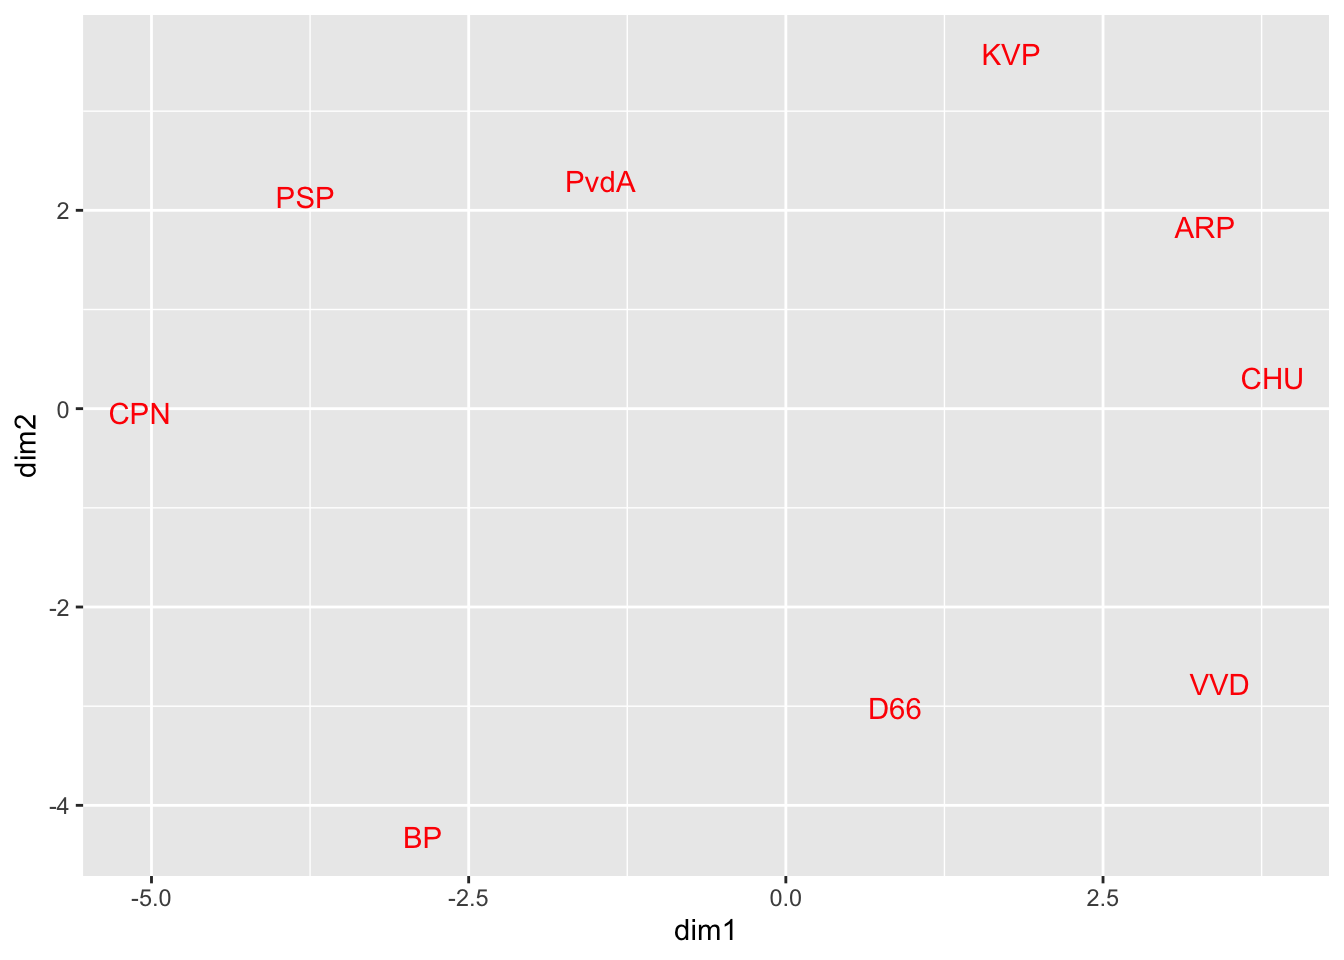
\includegraphics[keepaspectratio]{av_files/figure-pdf/pxls-1.pdf}}

}

\caption{Gruijter Configuration Least Squares}

\end{figure}%

\begin{figure}[H]

{\centering \pandocbounded{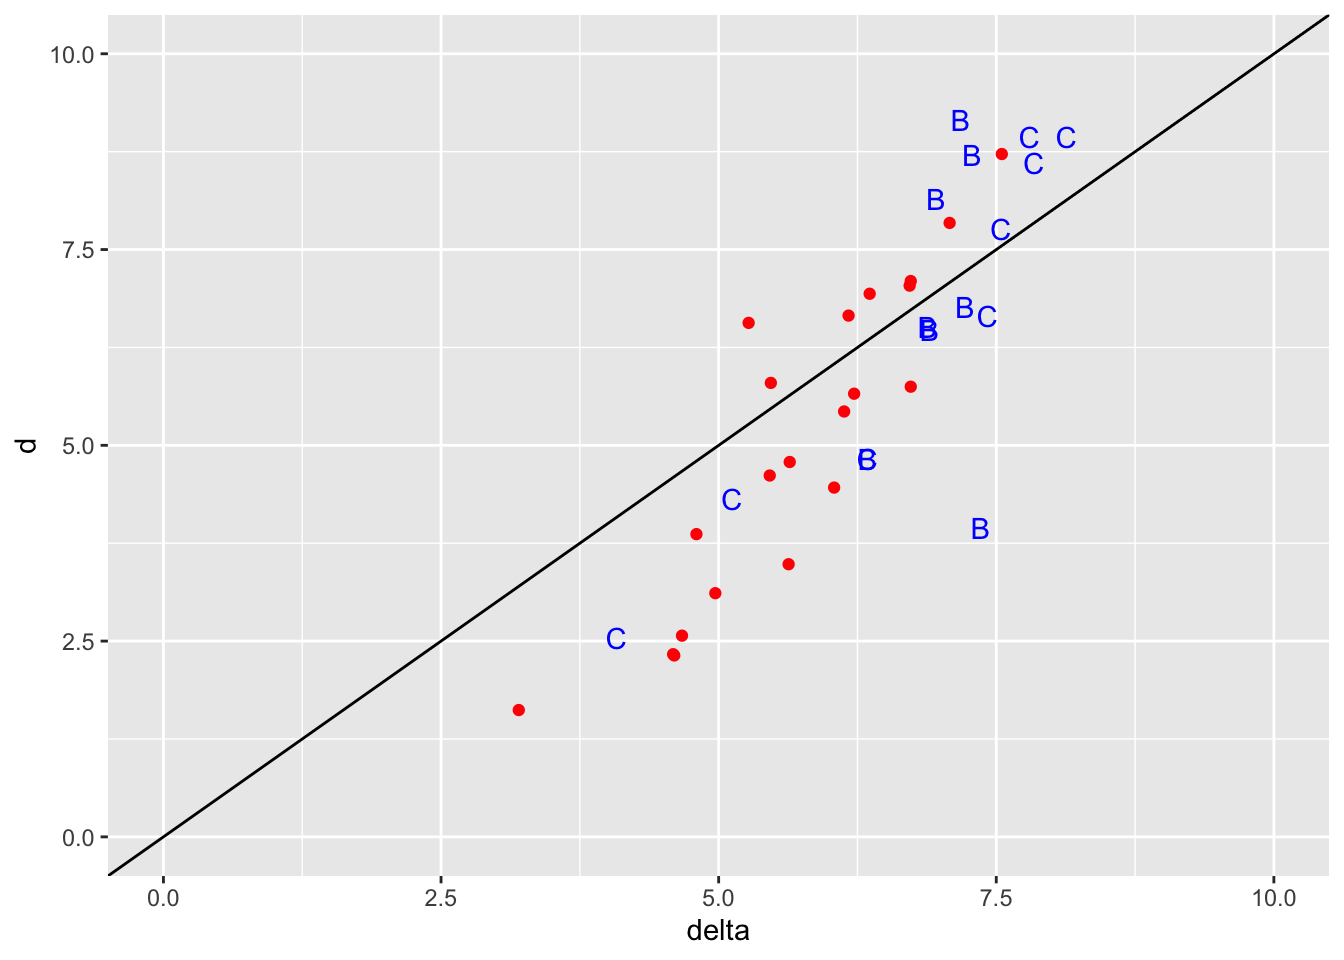
\includegraphics[keepaspectratio]{av_files/figure-pdf/pdls-1.pdf}}

}

\caption{Grujter Shepard Plot Least Squares}

\end{figure}%

The Shepard plot clearly shows why an additive constant would be very
beneficial in this case.

\begin{figure}[H]

{\centering \pandocbounded{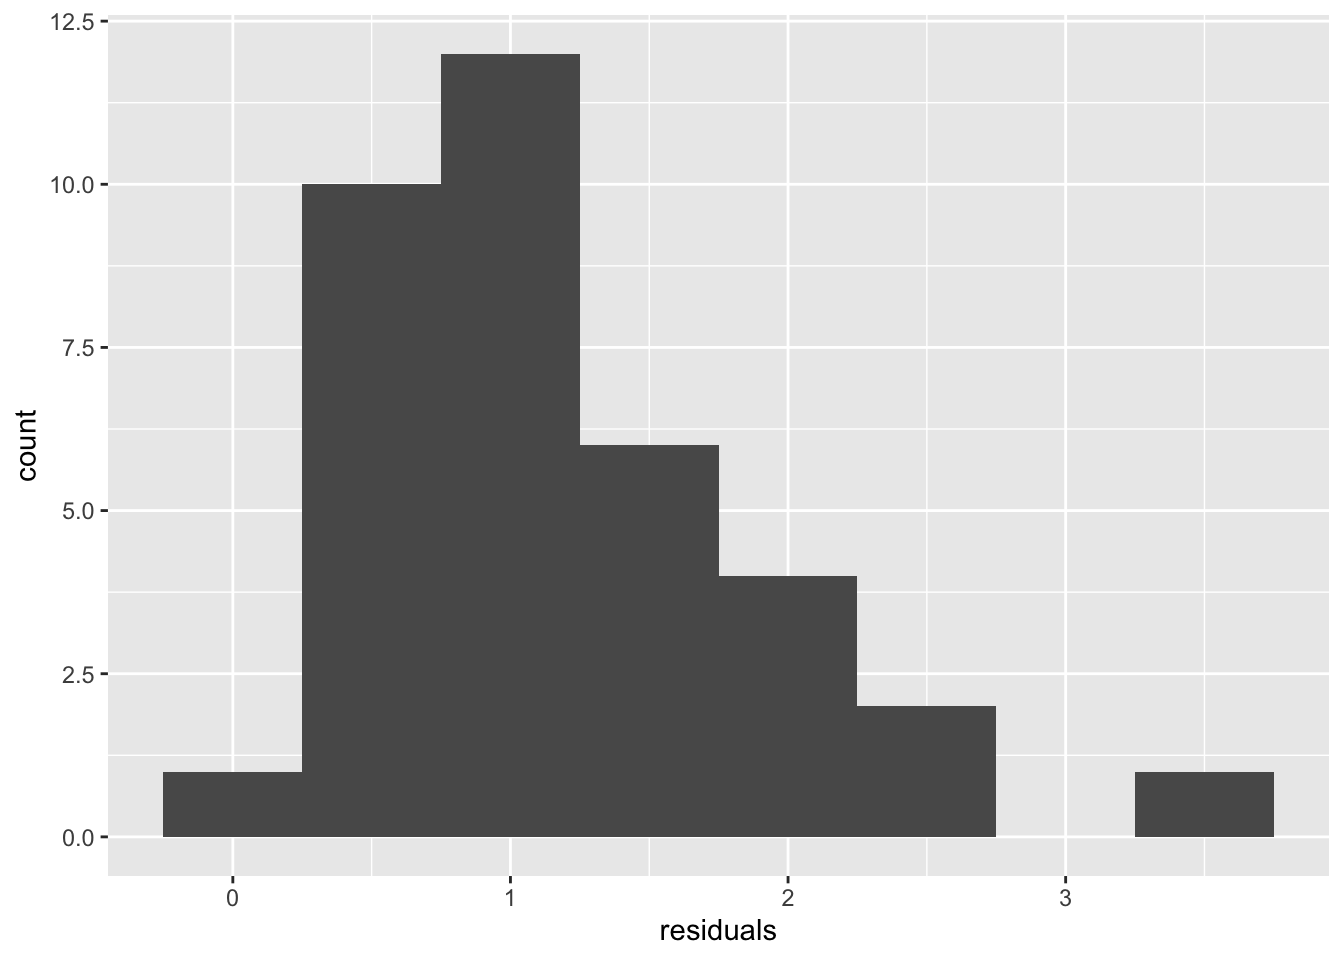
\includegraphics[keepaspectratio]{av_files/figure-pdf/phlsh-1.pdf}}

}

\caption{Gruijter Histogram Least Squares Residuals}

\end{figure}%

\subsubsection{Least Absolute Value}\label{least-absolute-value}

For our LAV smacof we use engine smacofCharbonnier with \(c=.001\). We
have convergence in 637 iterations.

\begin{figure}[H]

{\centering \pandocbounded{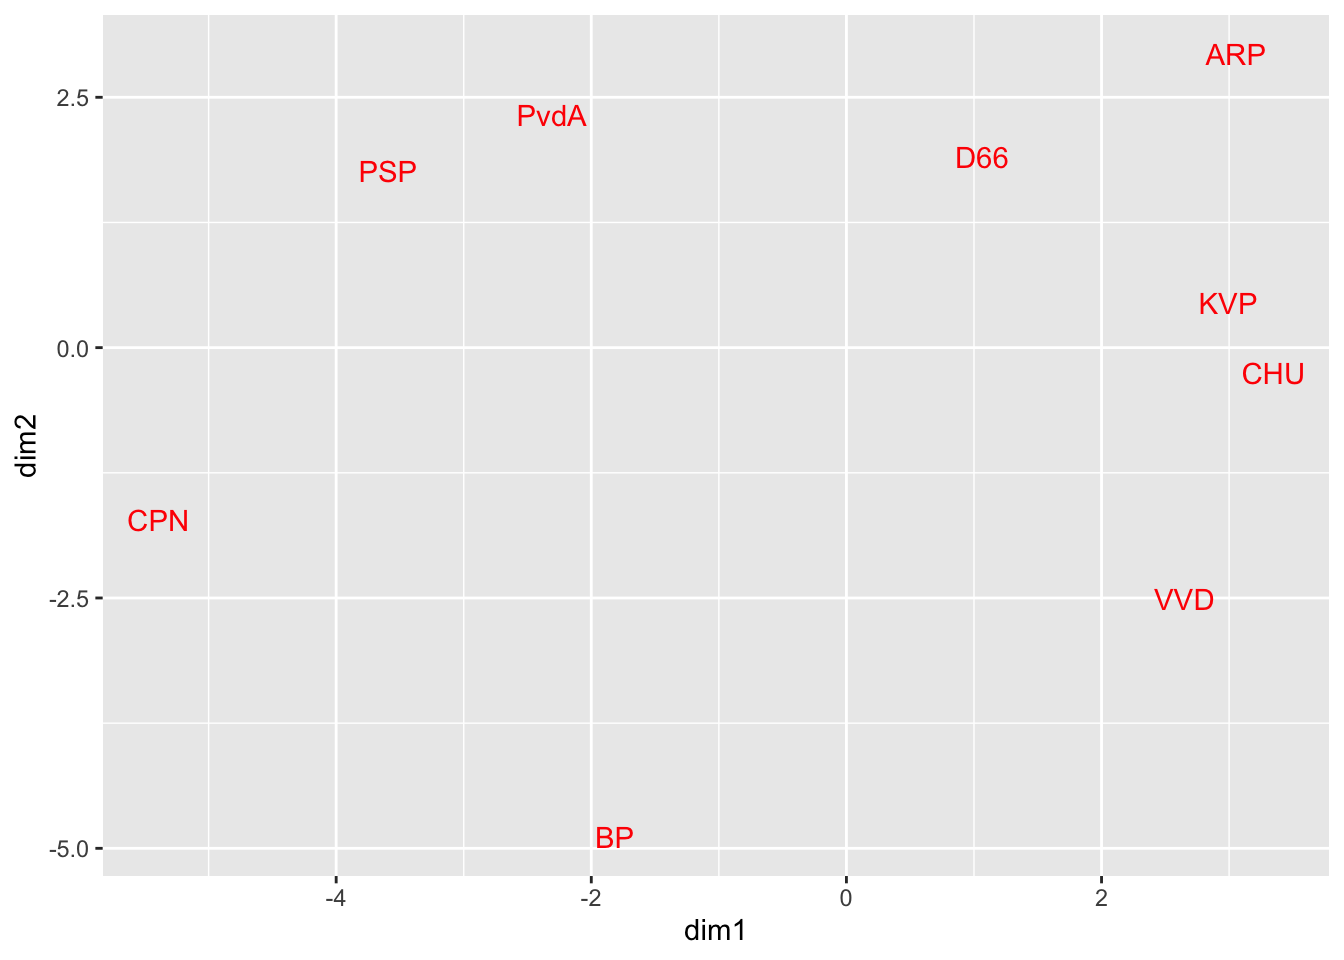
\includegraphics[keepaspectratio]{av_files/figure-pdf/pxav-1.pdf}}

}

\caption{Gruijter Configuration Least Absolute Value}

\end{figure}%

\begin{figure}[H]

{\centering \pandocbounded{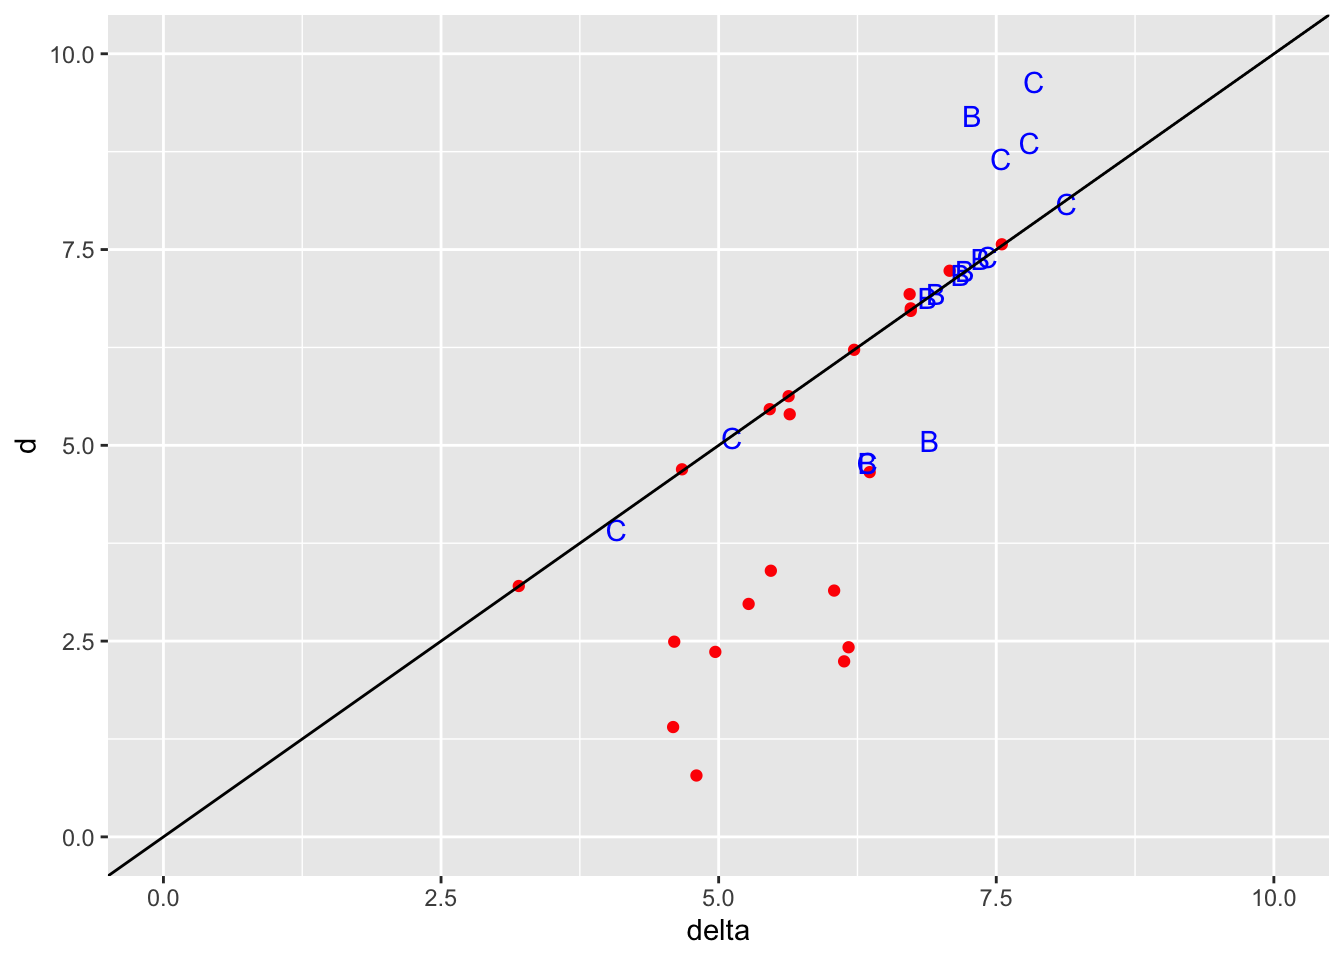
\includegraphics[keepaspectratio]{av_files/figure-pdf/pdav-1.pdf}}

}

\caption{Gruijter Shepard Plot Least Absolute Value}

\end{figure}%

In the Shepard plot we see that there are a number of dissimilarities
which are fitted exactly. If we count them there are about 15-20. Note
that configurations in two dimensions have \((n-1)+(n-2)=2n-3\) degrees
of freedom, which is 15 in this case. Thus if we take the 15
dissimilarities which are fitted exactly, give them weight one, give all
other 21 dissimilarities weight zero, and do a regular non-robust smacof
analysis using these weights, then we will have perfect fit in two
dimensions, and the solution will be the LAV solution. All this is
easier said than done, because it presumes that we use Charbonnier loss
with \(c=0\) and that we are able to decide which residuals are exactly
equal to zero. The LAV analysis also suggests the possibility of a huge
number of local minima, because there are so many ways to pick 15 out of
36 dissimilarities.

\begin{figure}[H]

{\centering \pandocbounded{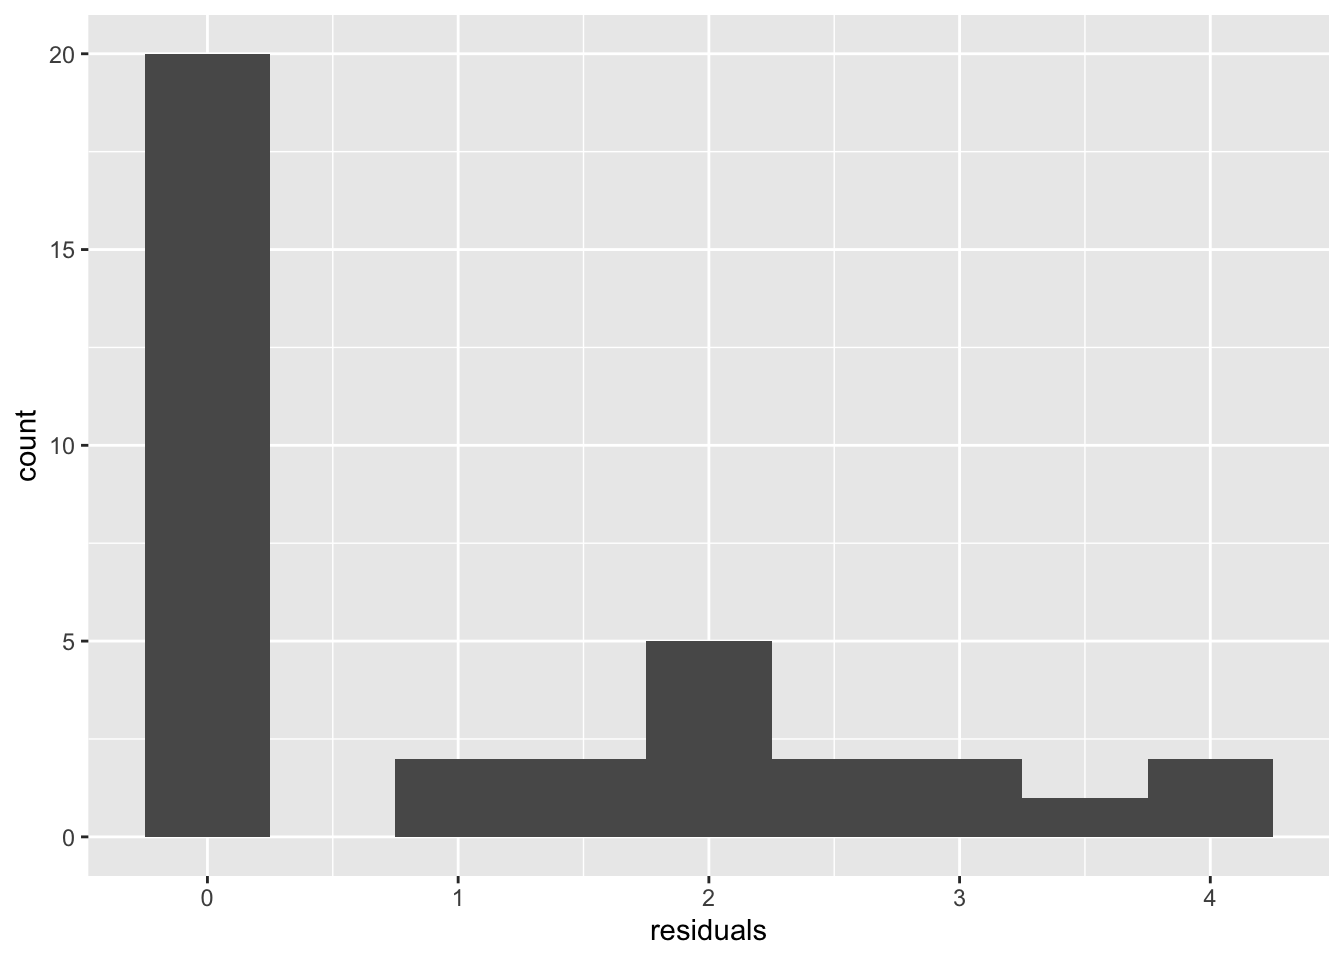
\includegraphics[keepaspectratio]{av_files/figure-pdf/phavh-1.pdf}}

}

\caption{Gruijter Histogram Least Absolute Value Residuals}

\end{figure}%

\subsubsection{Huber}\label{huber-1}

smacofHuber with \(c=1\) converges in 165 iterations.

\begin{figure}[H]

{\centering \pandocbounded{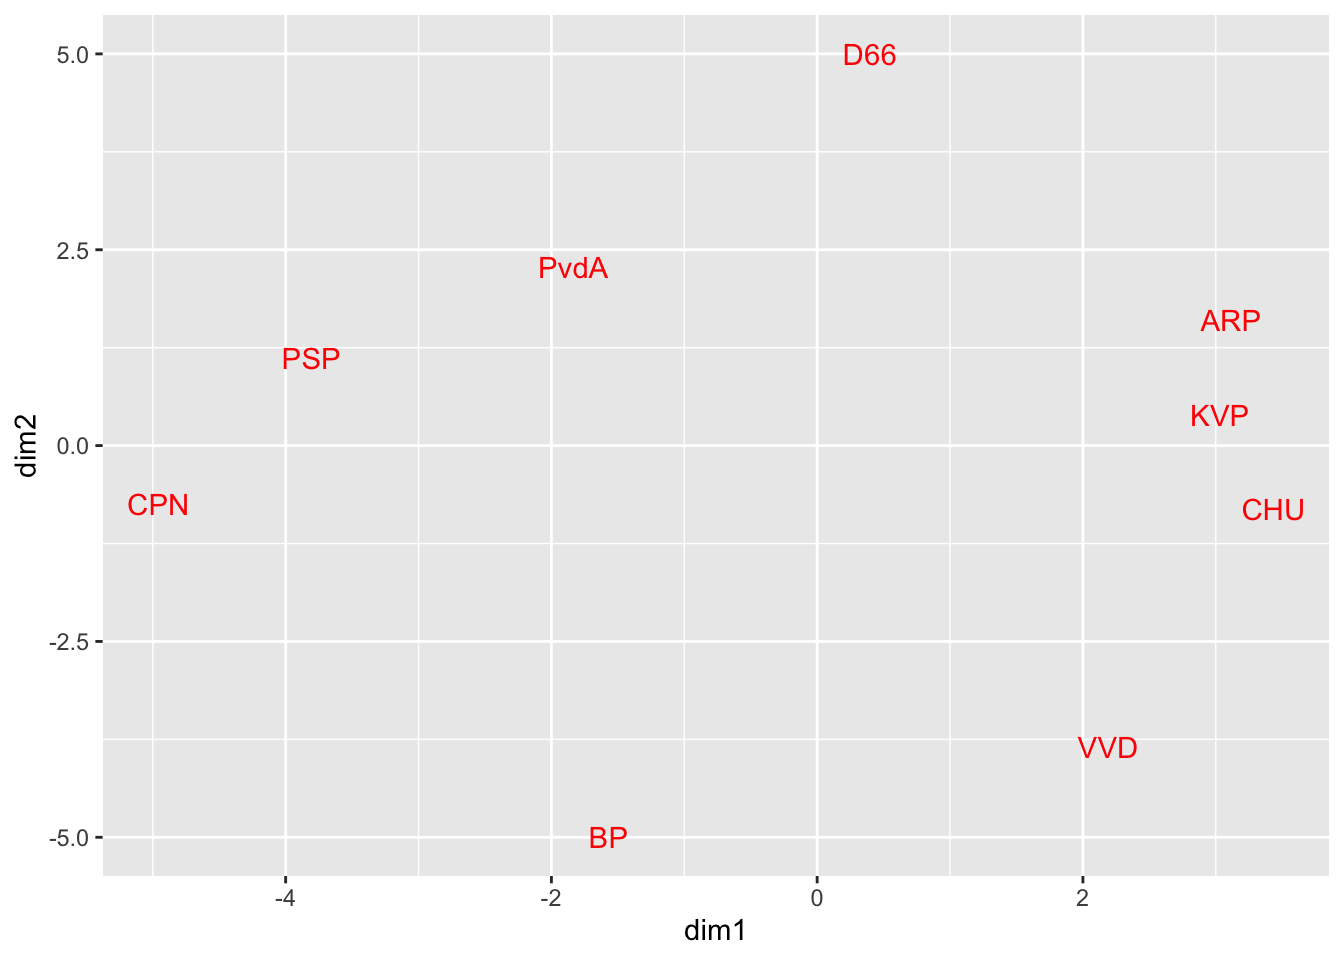
\includegraphics[keepaspectratio]{av_files/figure-pdf/pxhme-1.pdf}}

}

\caption{Gruijter Configuration Huber c = 1}

\end{figure}%

\begin{figure}[H]

{\centering \pandocbounded{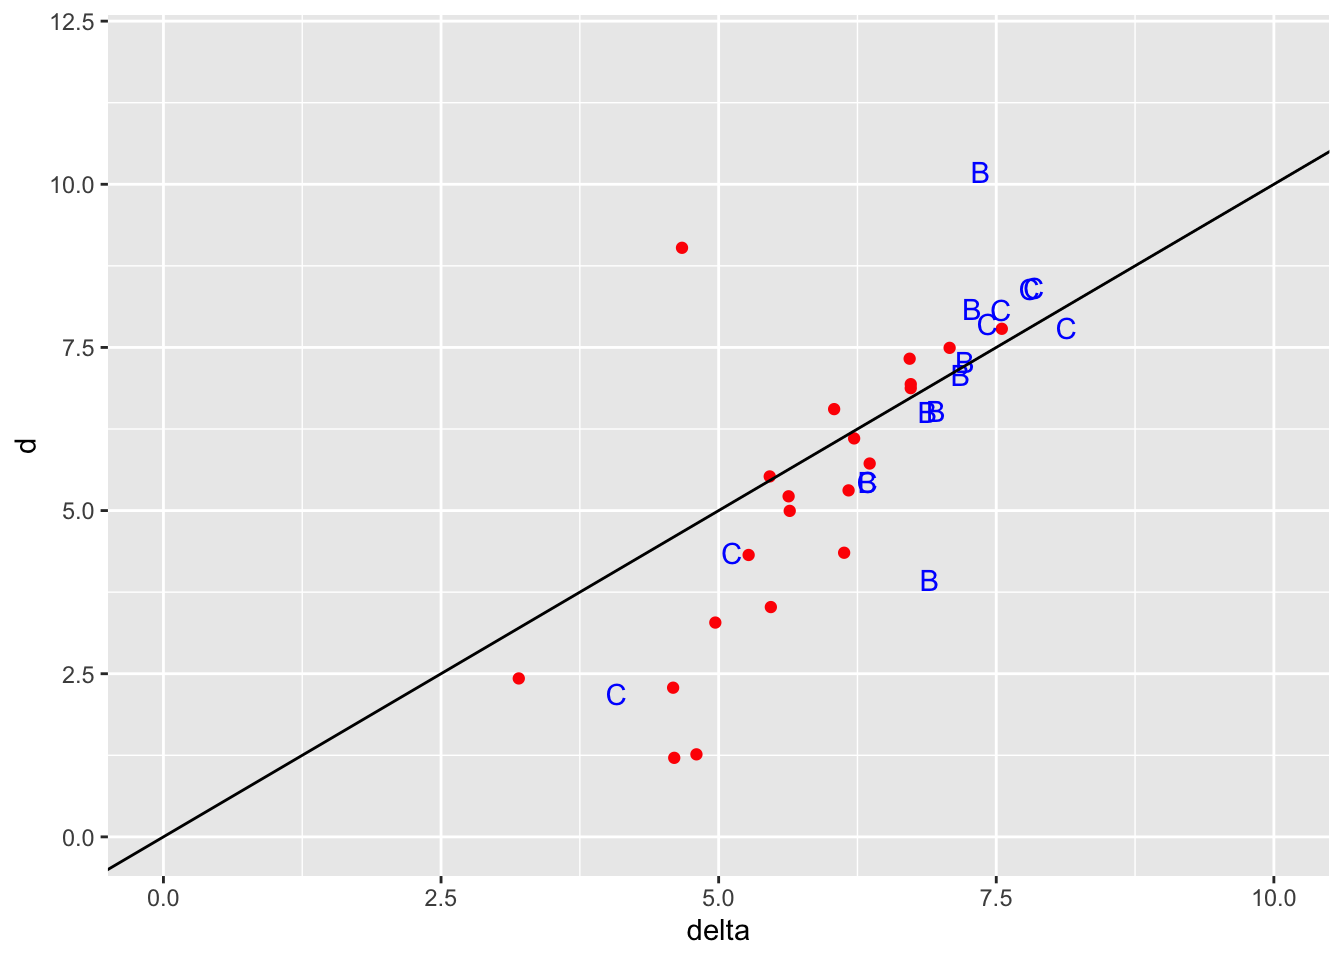
\includegraphics[keepaspectratio]{av_files/figure-pdf/pdhme-1.pdf}}

}

\caption{Gruijter Shepard Plot Huber c = 1}

\end{figure}%

\begin{figure}[H]

{\centering \pandocbounded{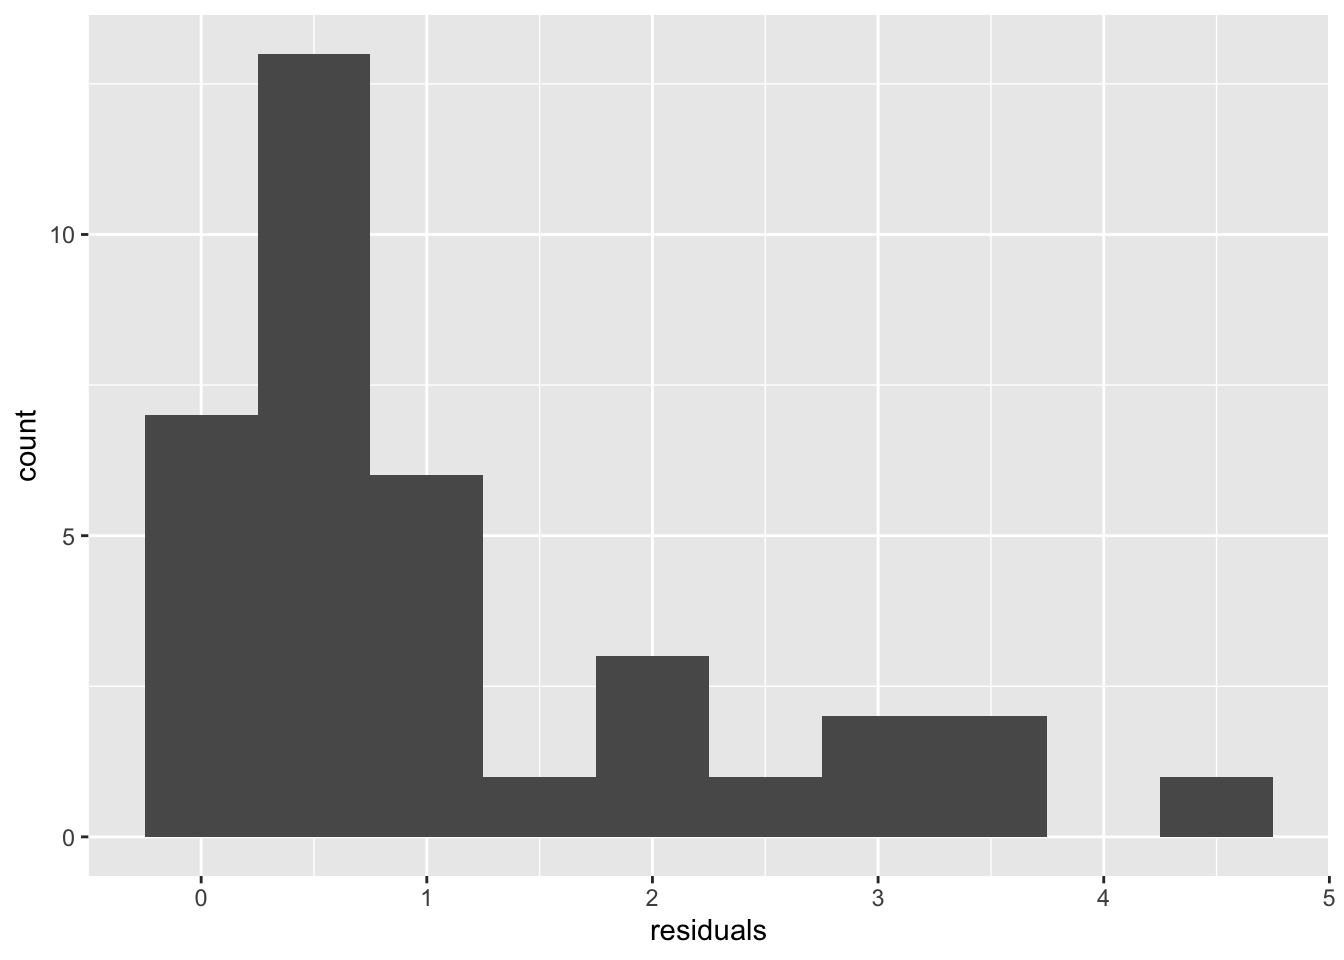
\includegraphics[keepaspectratio]{av_files/figure-pdf/phmeh-1.pdf}}

}

\caption{Gruijter Histogram Huber Residuals}

\end{figure}%

\subsubsection{Tukey}\label{tukey-1}

smacofTukey with \(c=2\) converges in 180 iterations.

\begin{figure}[H]

{\centering \pandocbounded{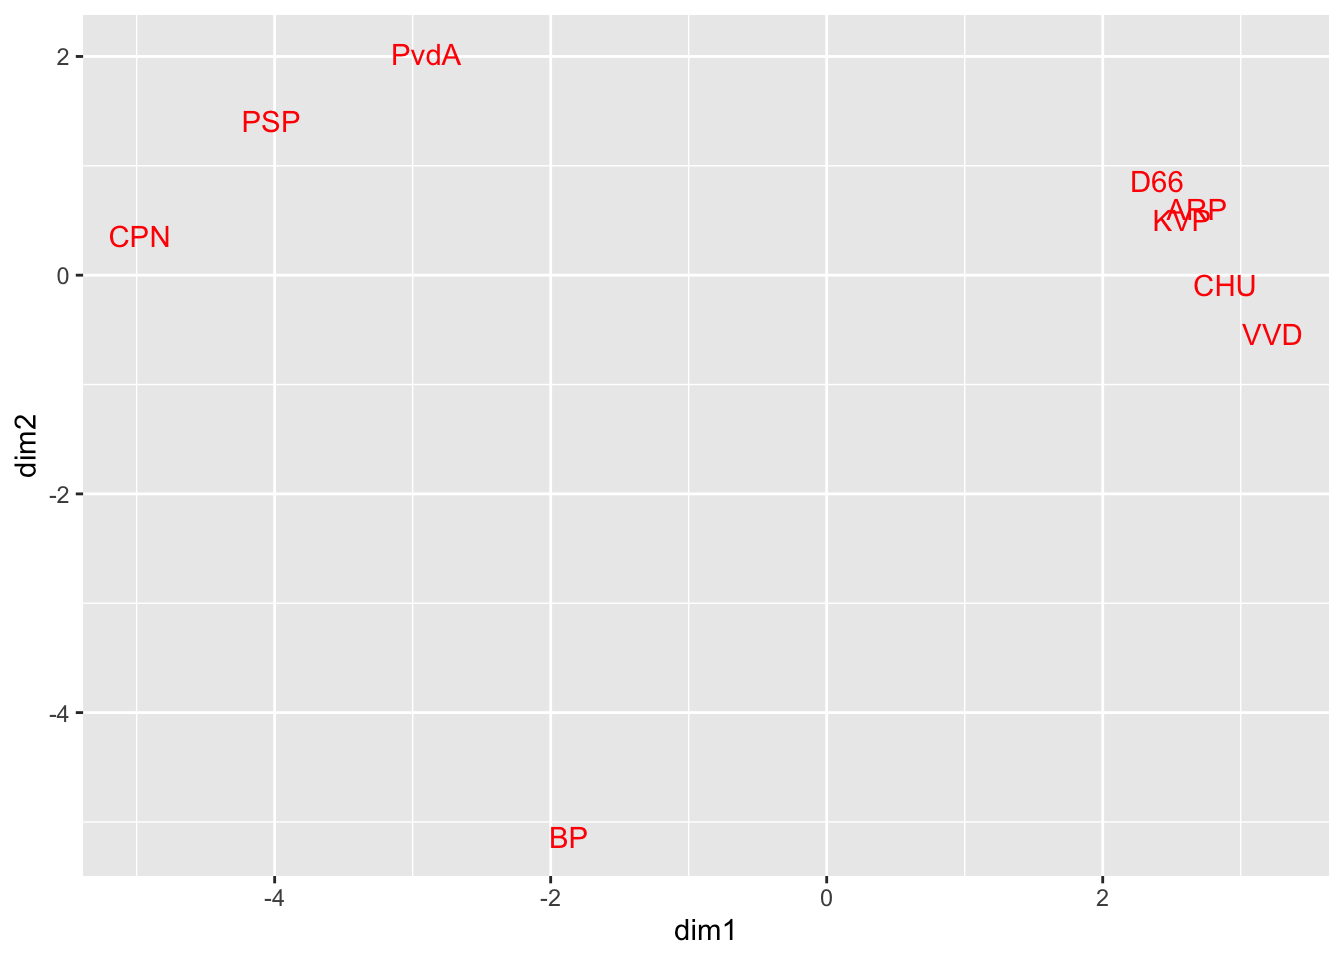
\includegraphics[keepaspectratio]{av_files/figure-pdf/pxtmed-1.pdf}}

}

\caption{Gruijter Configuration Tukey c = 2}

\end{figure}%

\begin{figure}[H]

{\centering \pandocbounded{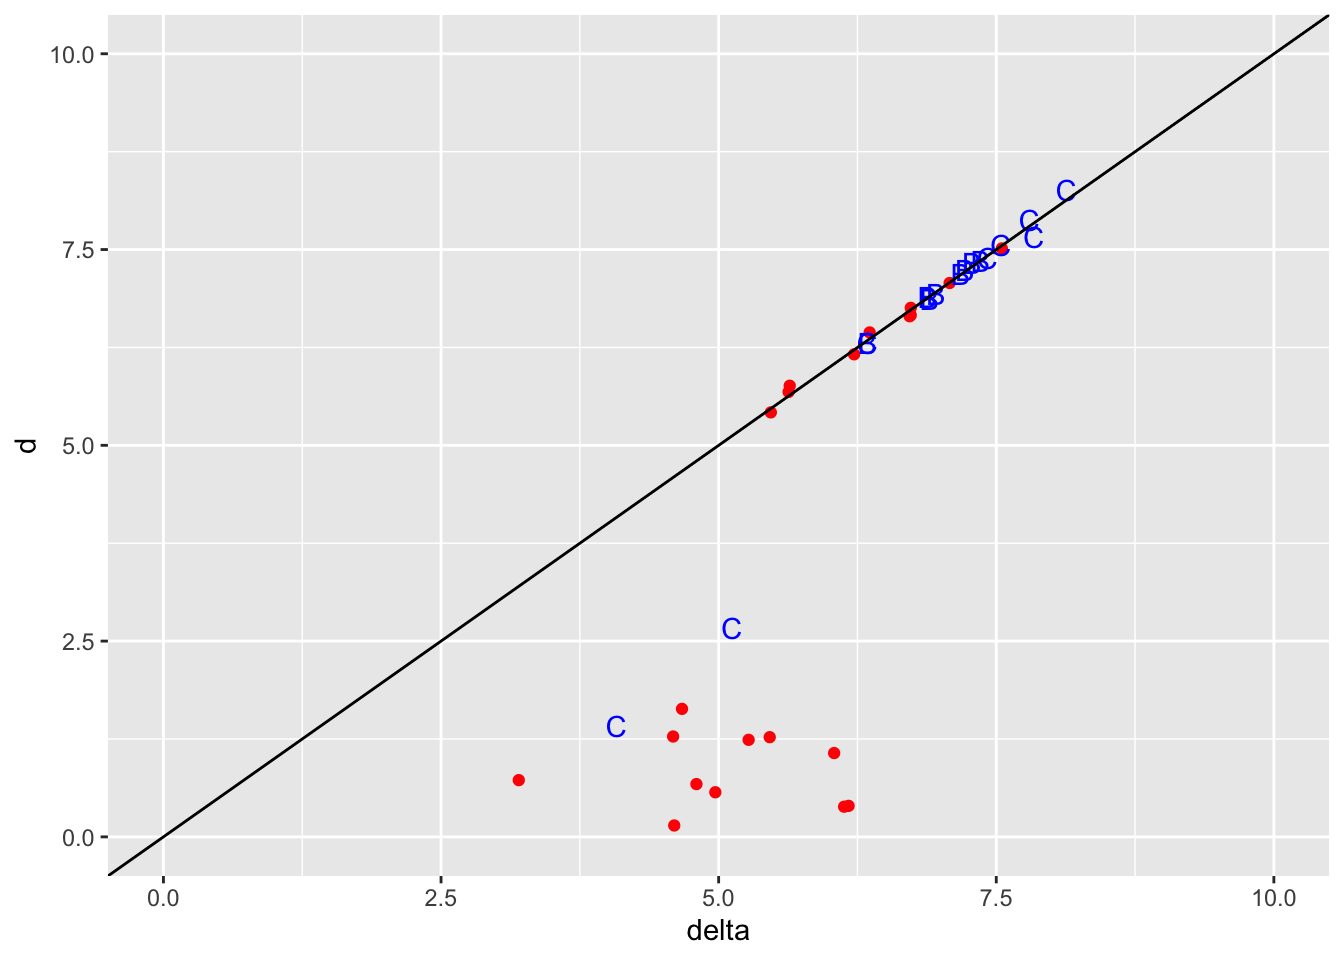
\includegraphics[keepaspectratio]{av_files/figure-pdf/pdtmed-1.pdf}}

}

\caption{Gruijter Shepard Plot Tukey c = 2}

\end{figure}%

\begin{figure}[H]

{\centering \pandocbounded{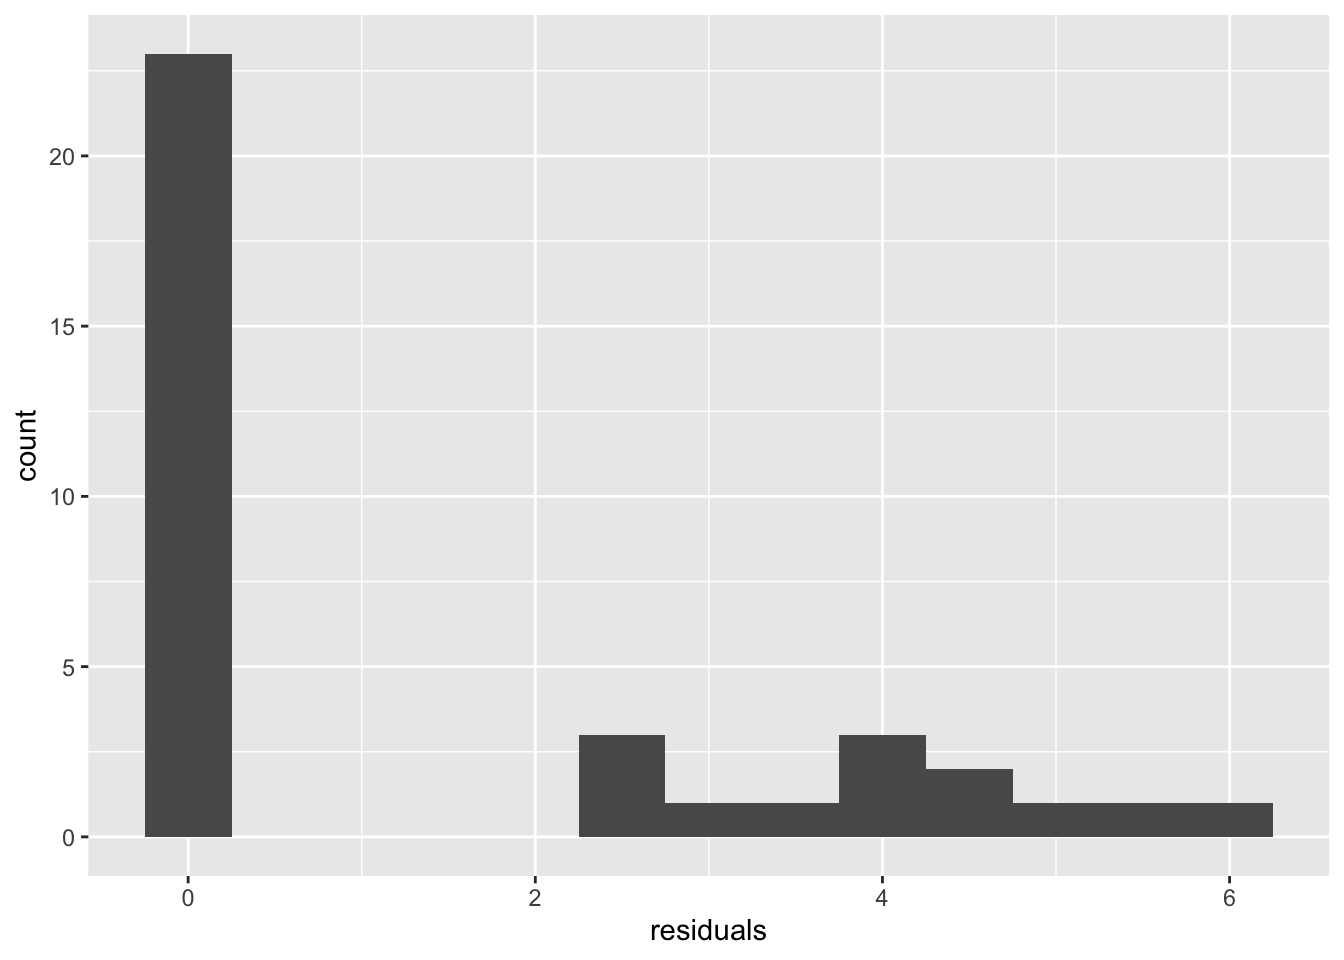
\includegraphics[keepaspectratio]{av_files/figure-pdf/phtuh-1.pdf}}

}

\caption{Gruijter Histogram Tukey Residuals}

\end{figure}%

\subsection{Rothkopf}\label{rothkopf}

Our second example are the Rothkopf Morse data (Rothkopf
(\citeproc{ref-rothkopf_57}{1957})), which have a better fit and have
fewer outliers than the Gruijter data. We used the asymetric confusion
matrix from the smacof package (De Leeuw and Mair
(\citeproc{ref-deleeuw_mair_A_09c}{2009})) and defined dissimilarities
by the Shepard-Luce formula \[
\delta_{ij}=-\log\frac{p_{ij}p_{ji}}{p_{ii}p_{jj}}.
\]

\subsubsection{Least Squares}\label{least-squares-1}

For least squares we use the smacofHuber engine with \(c=25\), well
outside the range of the residuals. We have convergence in 213
iterations.

\begin{figure}[H]

{\centering \pandocbounded{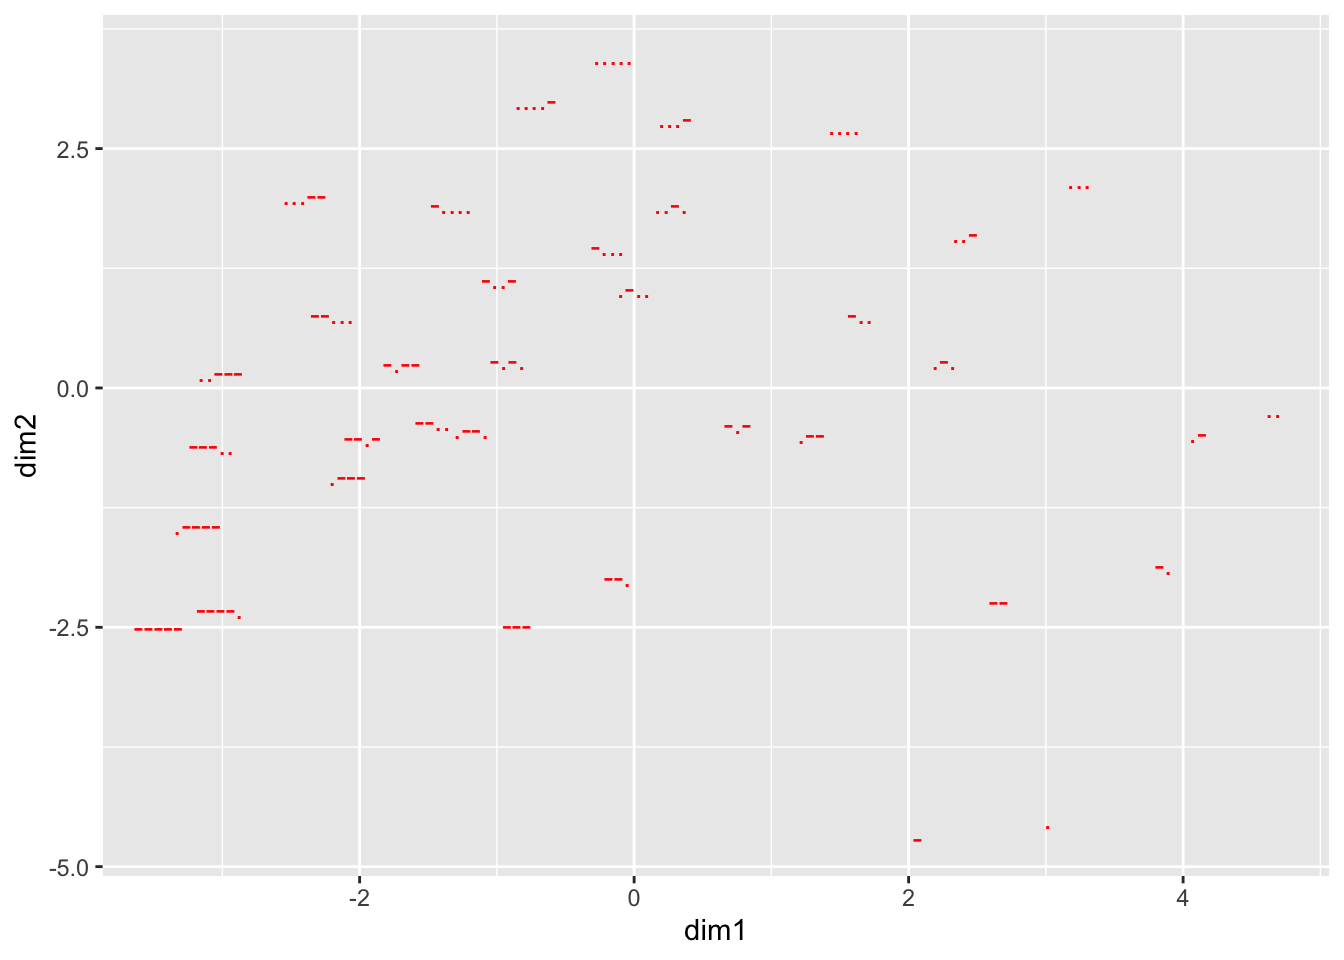
\includegraphics[keepaspectratio]{av_files/figure-pdf/mpxls-1.pdf}}

}

\caption{Rothkopf Configuration Least Squares}

\end{figure}%

\begin{figure}[H]

{\centering \pandocbounded{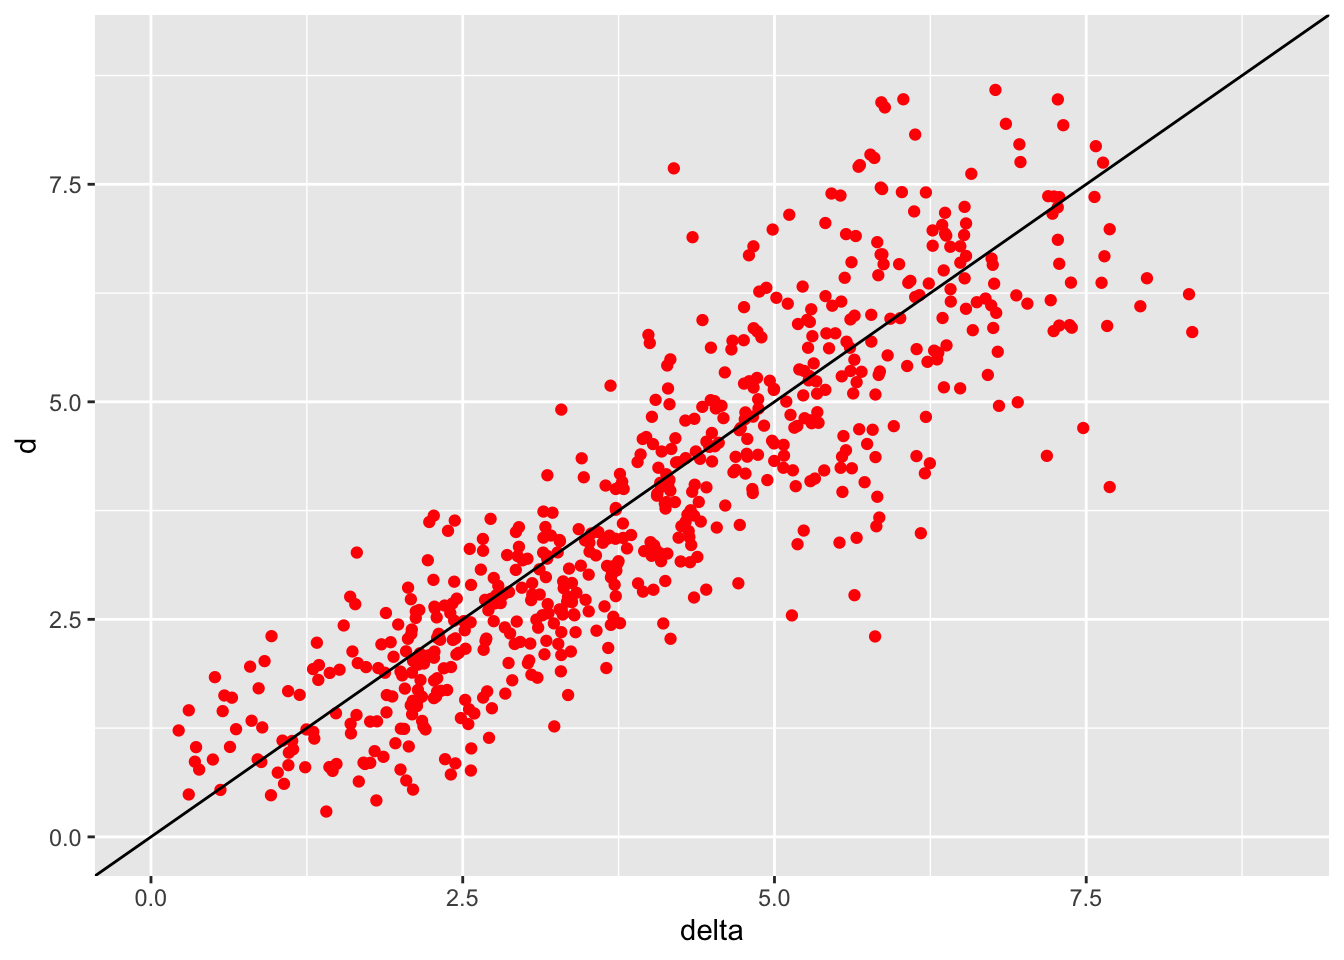
\includegraphics[keepaspectratio]{av_files/figure-pdf/mkpdls-1.pdf}}

}

\caption{Rothkopf Shepard Plot Least Squares}

\end{figure}%

\begin{figure}[H]

{\centering \pandocbounded{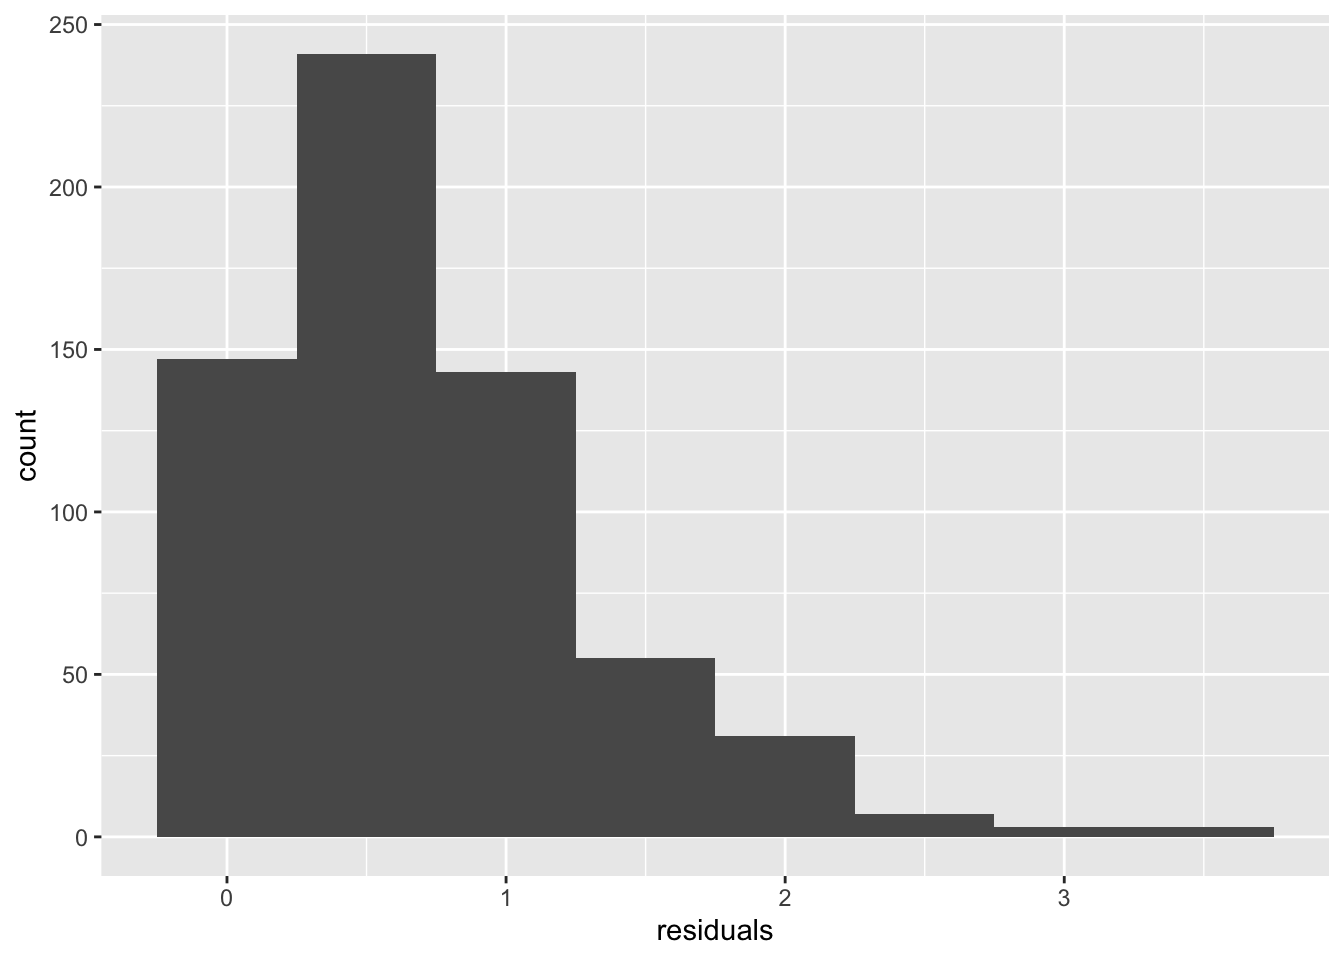
\includegraphics[keepaspectratio]{av_files/figure-pdf/mphlsh-1.pdf}}

}

\caption{Rothkopf Histogram Least Squares Residuals}

\end{figure}%

\subsubsection{Least Absolute Value}\label{least-absolute-value-1}

For least absolute value we use Chardonnier loss with \(c=.001\). We
have convergence in 2291 iterations.

\begin{figure}[H]

{\centering \pandocbounded{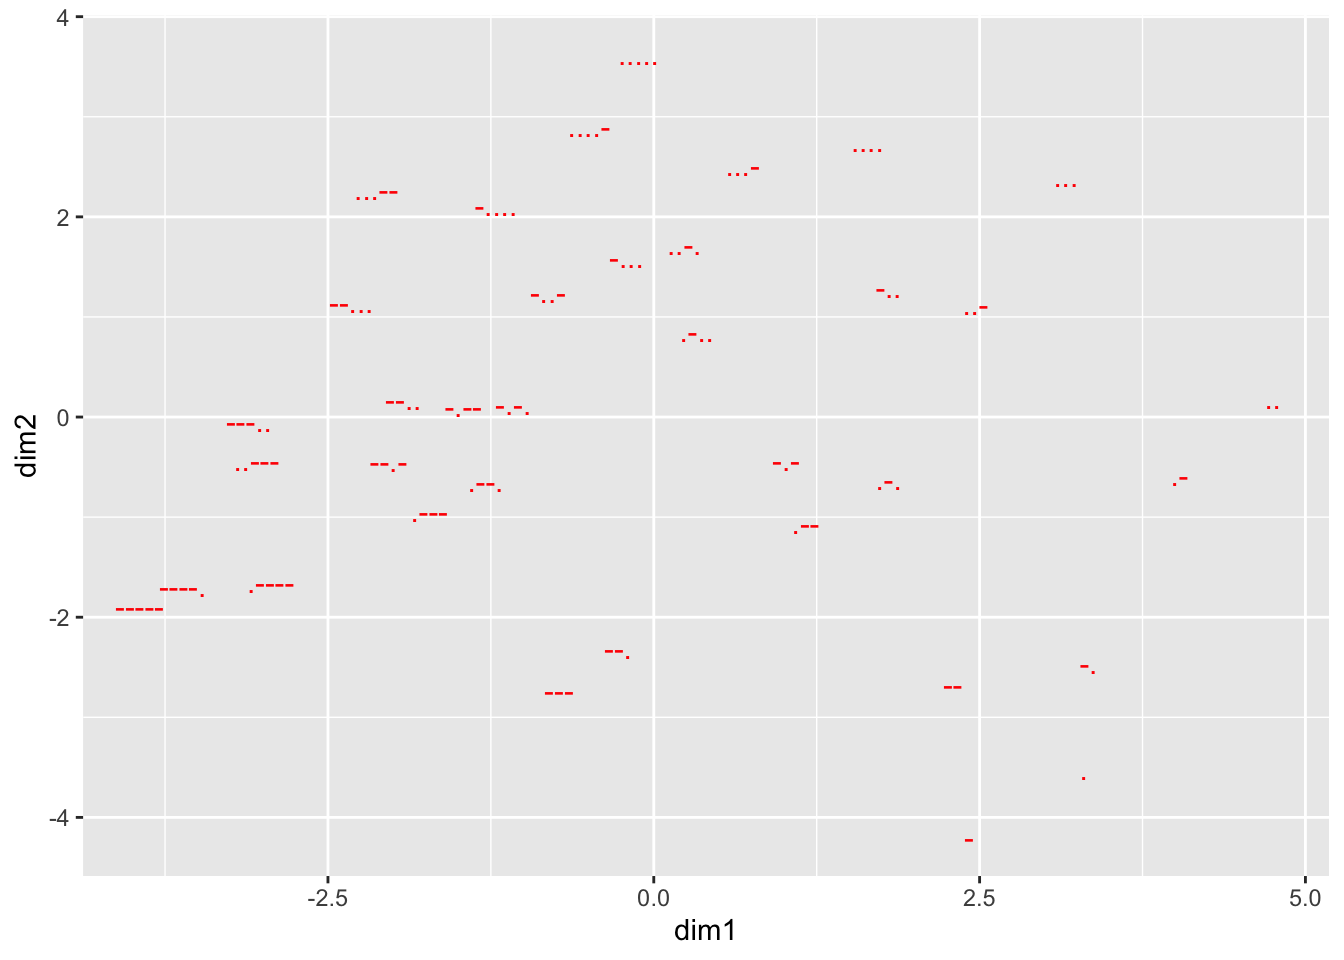
\includegraphics[keepaspectratio]{av_files/figure-pdf/mpxav-1.pdf}}

}

\caption{Rothkopf Configuration Least Absolute Value}

\end{figure}%

\begin{figure}[H]

{\centering \pandocbounded{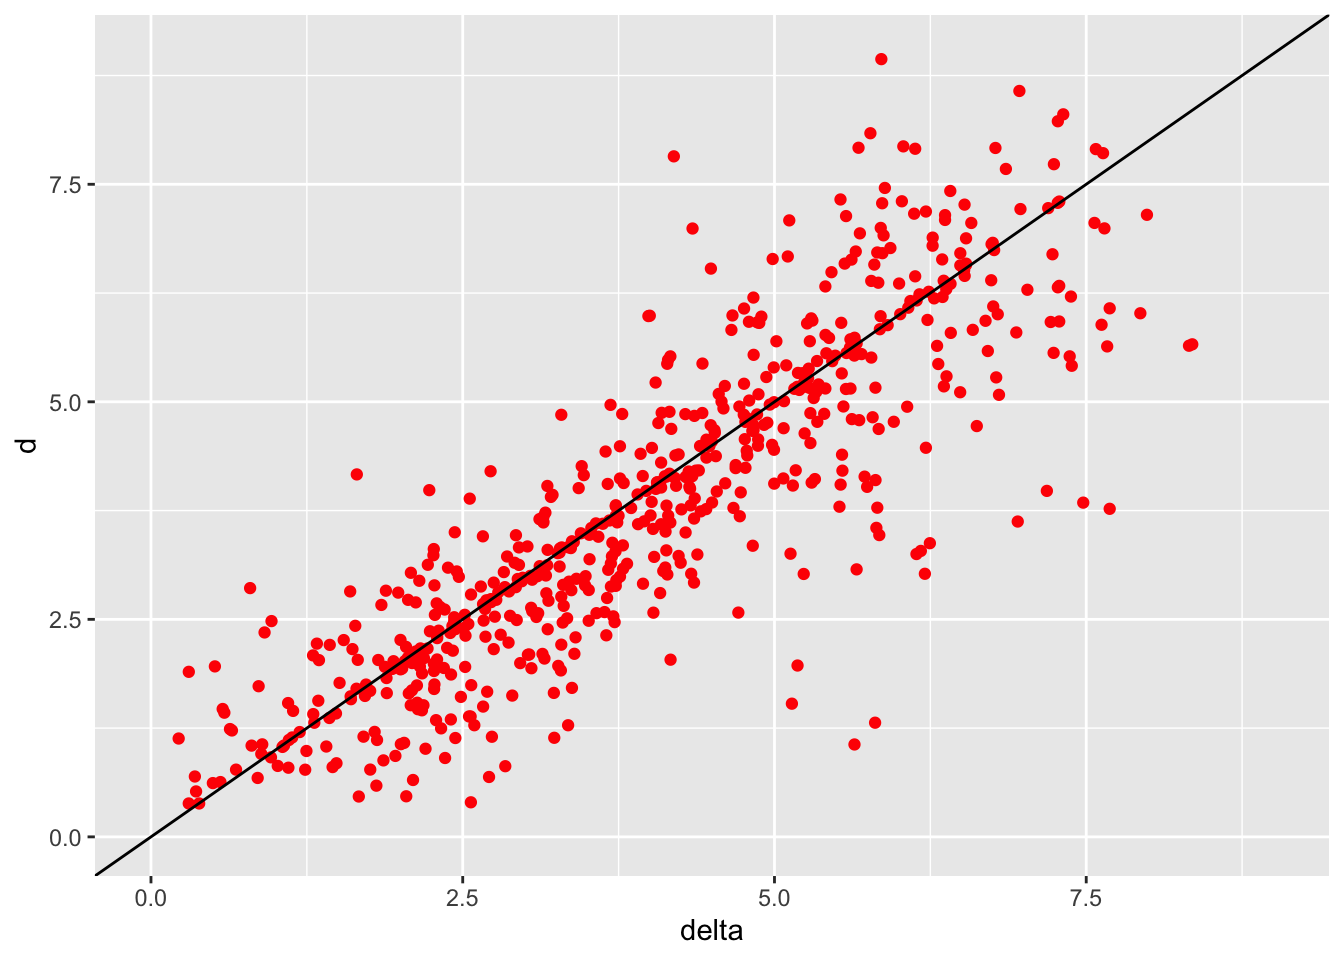
\includegraphics[keepaspectratio]{av_files/figure-pdf/mpdav-1.pdf}}

}

\caption{Rothkopf Shepard Plot Least Absolute Value}

\end{figure}%

\begin{figure}[H]

{\centering \pandocbounded{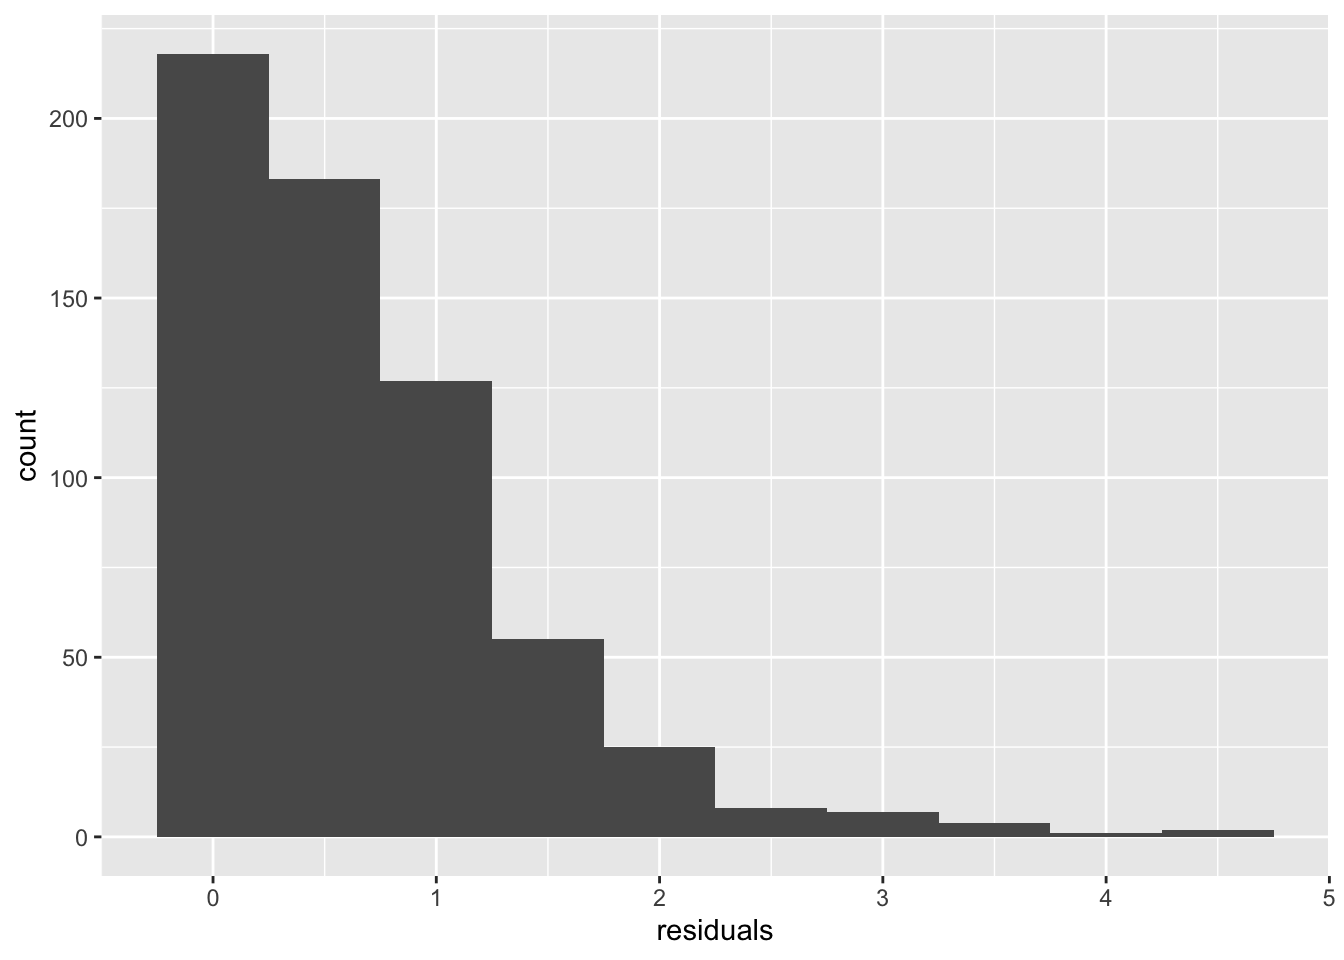
\includegraphics[keepaspectratio]{av_files/figure-pdf/mphlavh-1.pdf}}

}

\caption{Rothkopf Histogram Least Absolute Value Residuals}

\end{figure}%

\subsubsection{Huber}\label{huber-2}

smacofHuber with \(c=1\) converges in 680 iterations.

\begin{figure}[H]

{\centering \pandocbounded{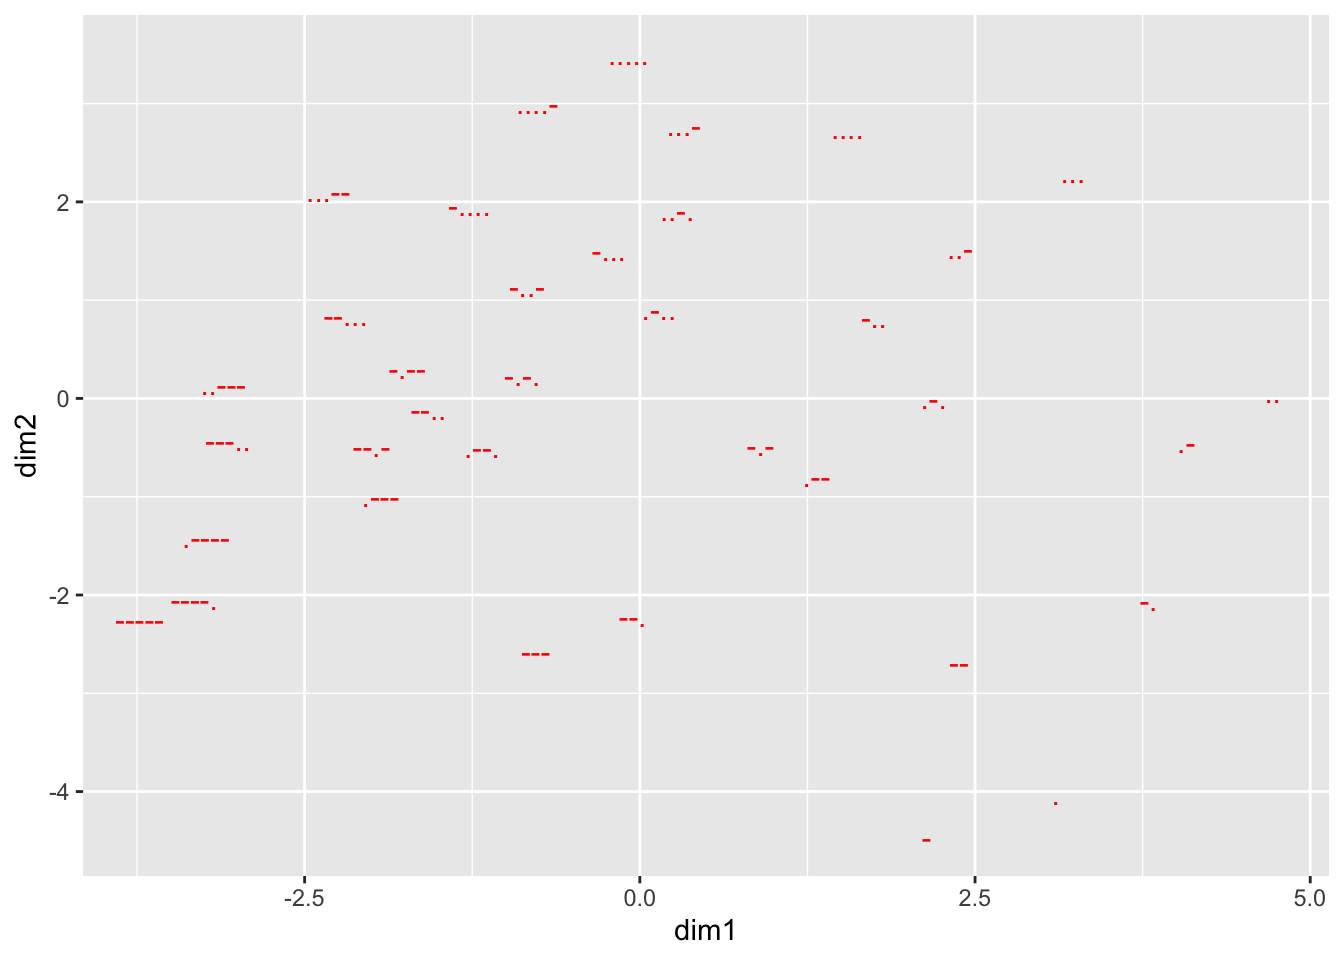
\includegraphics[keepaspectratio]{av_files/figure-pdf/mpxhme-1.pdf}}

}

\caption{Rothkopf Configuration Huber c = 1}

\end{figure}%

\begin{figure}[H]

{\centering \pandocbounded{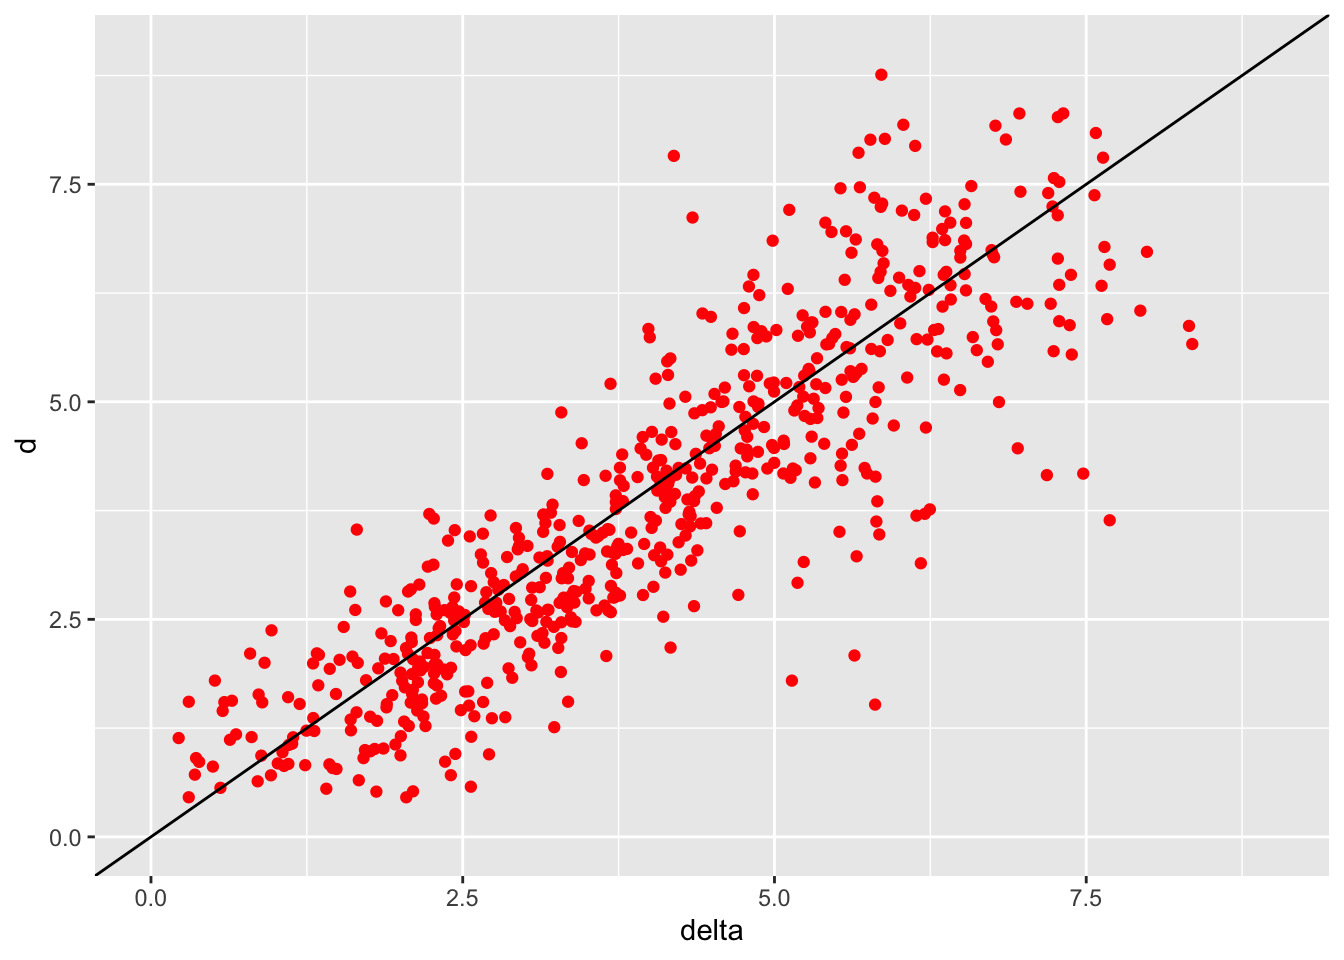
\includegraphics[keepaspectratio]{av_files/figure-pdf/mpdhme-1.pdf}}

}

\caption{Rothkopf Shepard Plot Huber c = 1}

\end{figure}%

\begin{figure}[H]

{\centering \pandocbounded{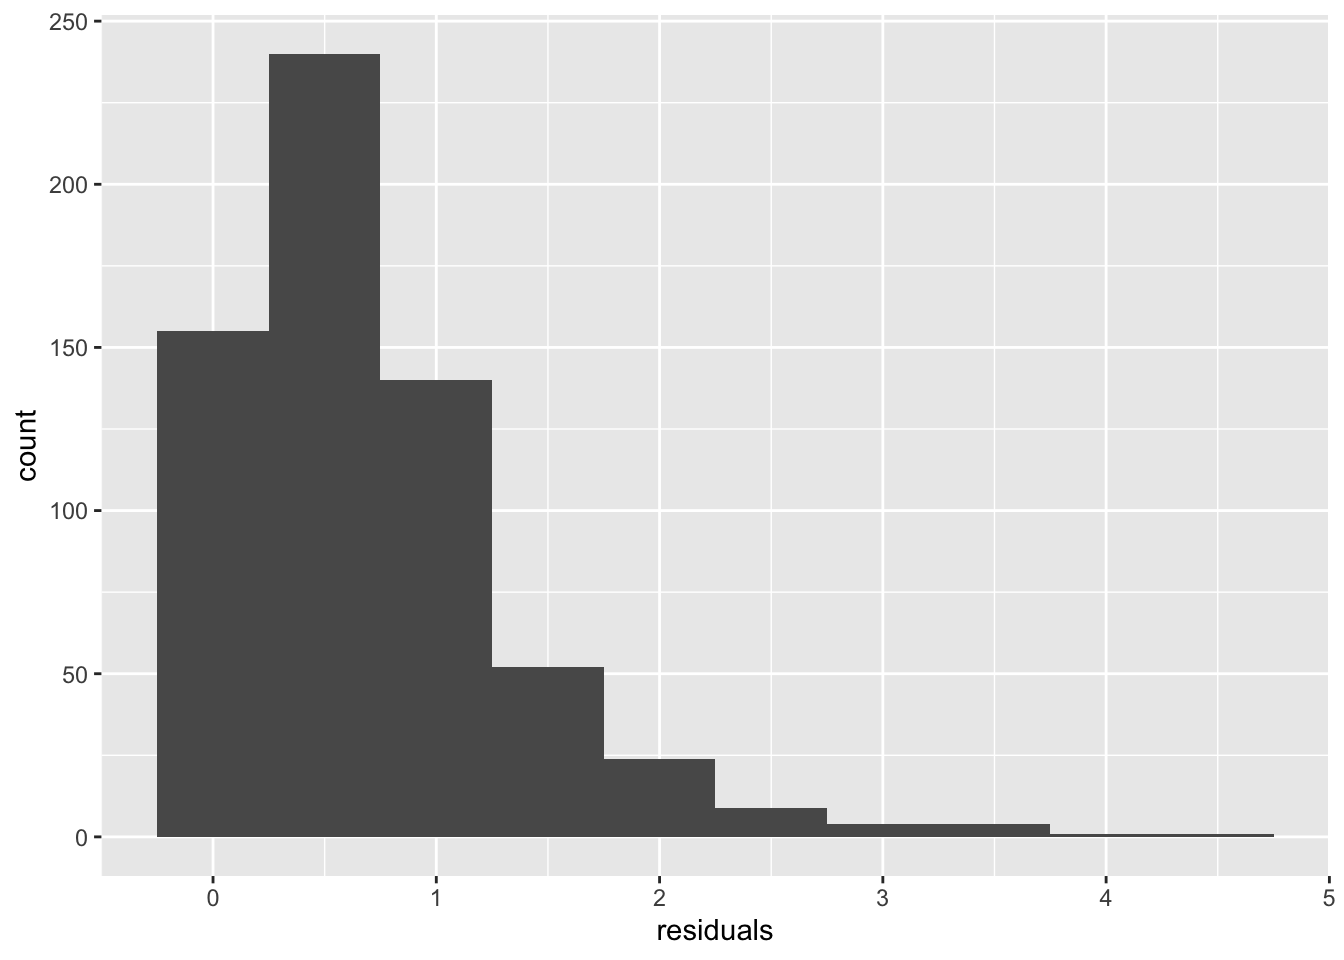
\includegraphics[keepaspectratio]{av_files/figure-pdf/mphmeh-1.pdf}}

}

\caption{Rothkopf Histogram Huber Residuals}

\end{figure}%

\subsubsection{Tukey}\label{tukey-2}

Tukey with \(c=1\) converges in 812 iterations.

\begin{figure}[H]

{\centering \pandocbounded{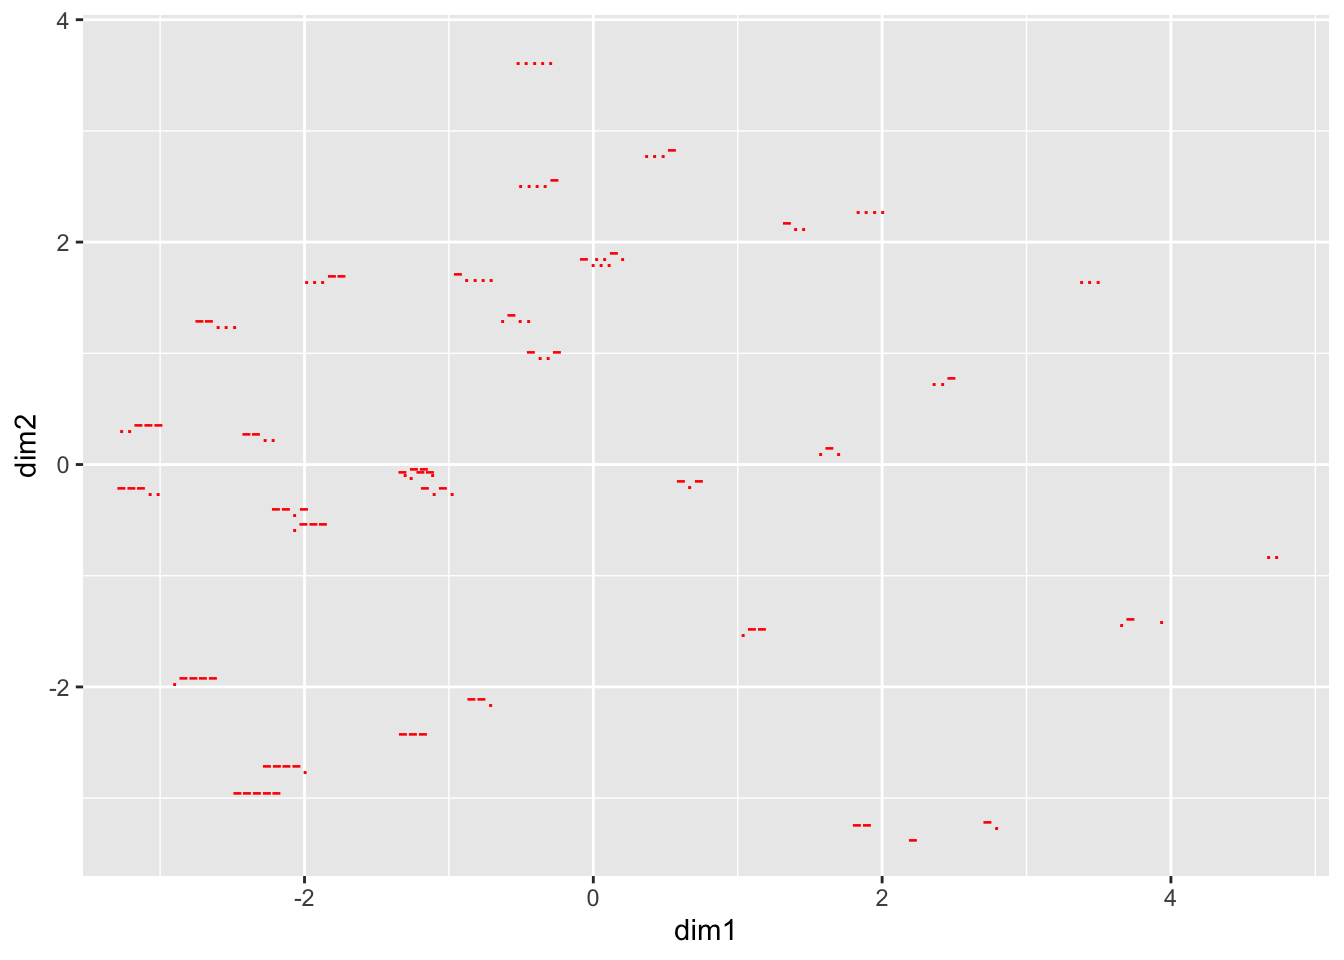
\includegraphics[keepaspectratio]{av_files/figure-pdf/mpxtu-1.pdf}}

}

\caption{Rothkopf Configuration Tukey c = 1}

\end{figure}%

\begin{figure}[H]

{\centering \pandocbounded{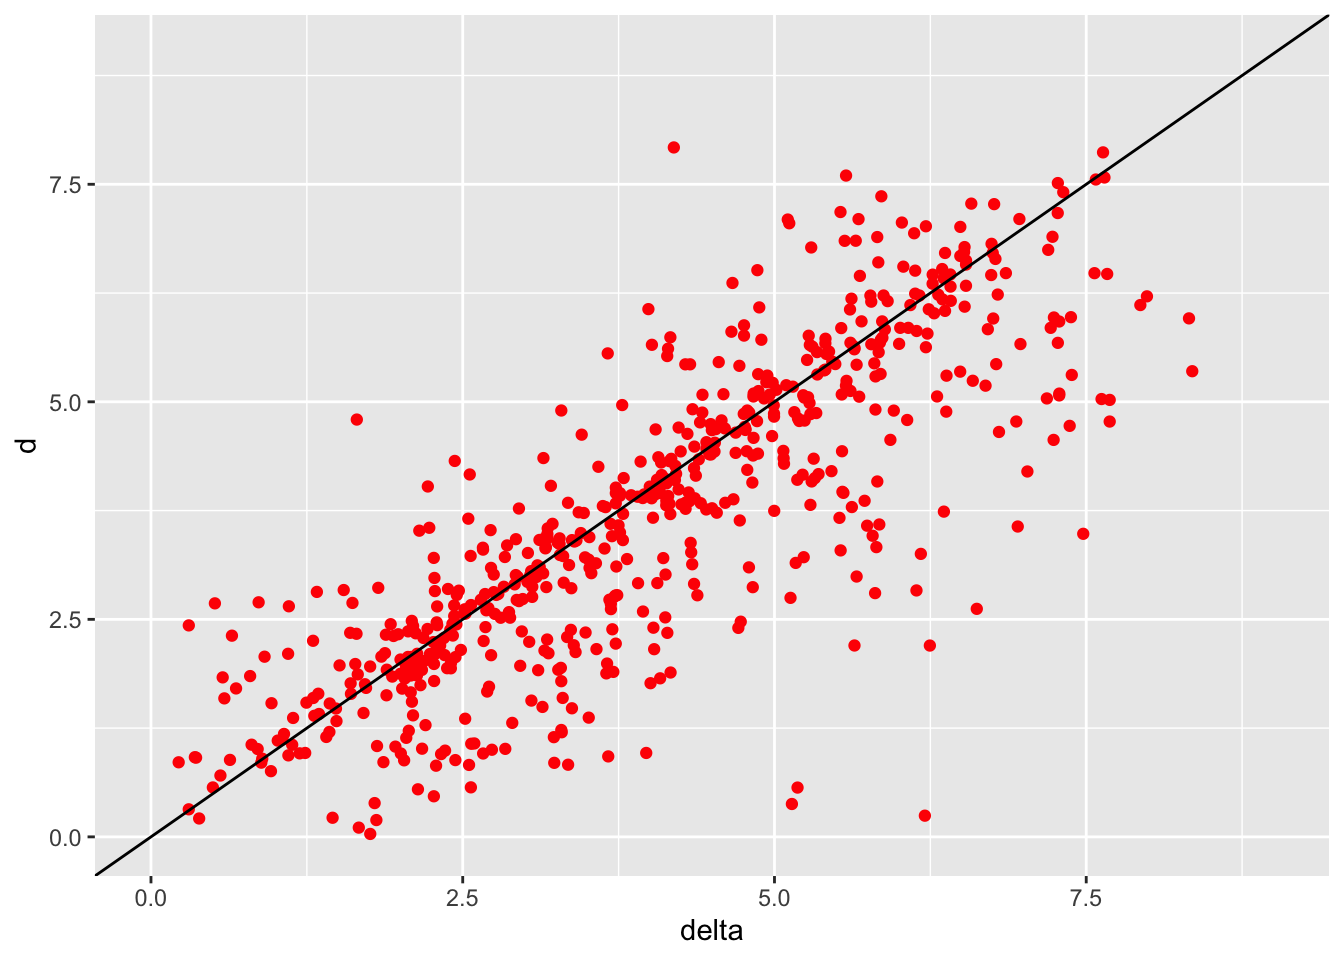
\includegraphics[keepaspectratio]{av_files/figure-pdf/pdttu-1.pdf}}

}

\caption{Rothkopf Shepard Plot Tukey c = 1}

\end{figure}%

\begin{figure}[H]

{\centering \pandocbounded{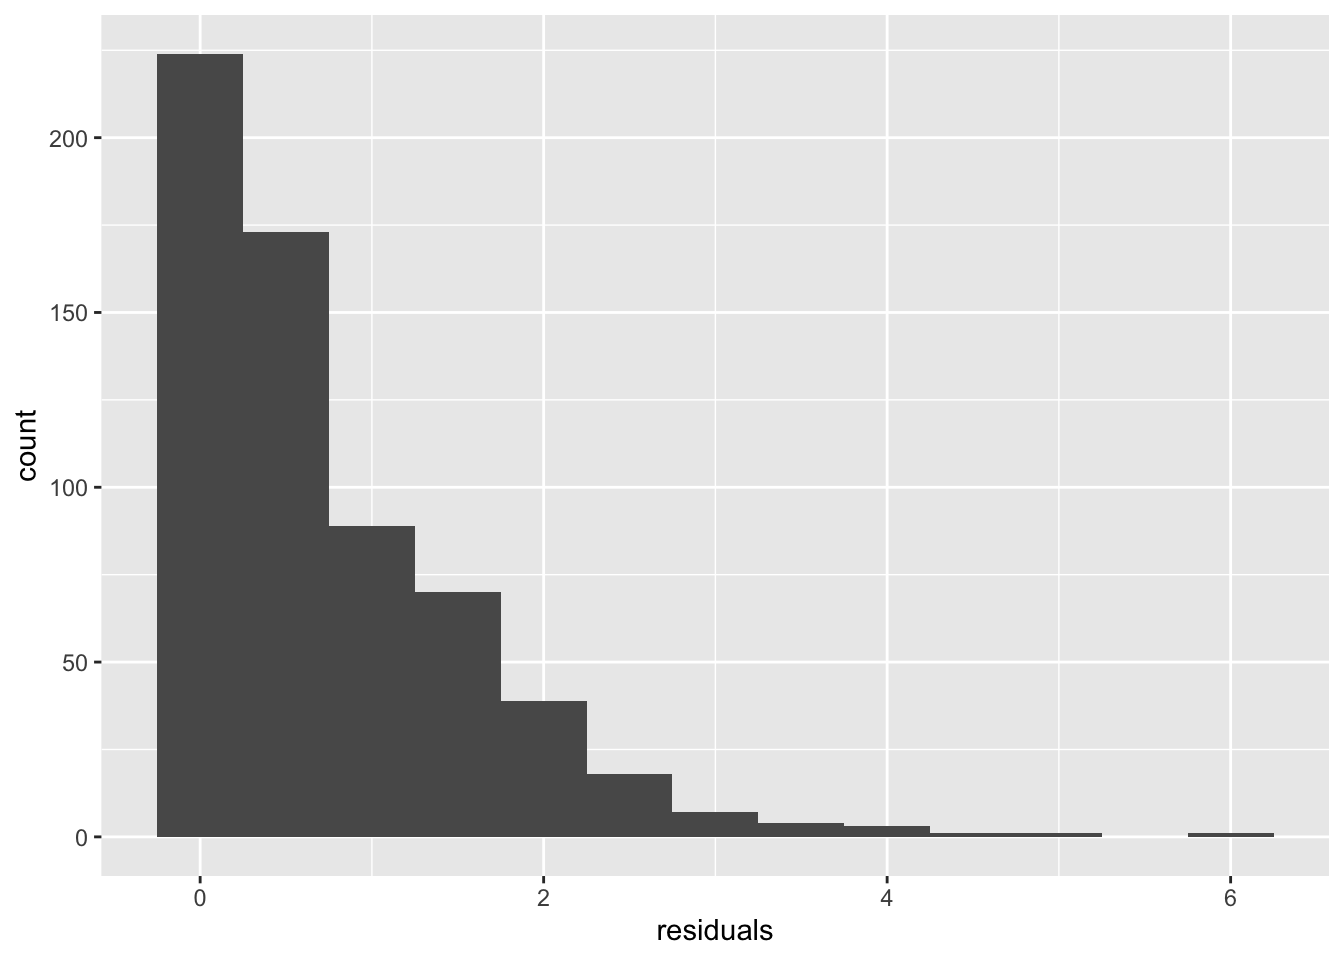
\includegraphics[keepaspectratio]{av_files/figure-pdf/mphtuh-1.pdf}}

}

\caption{Rothkopf Histogram Tukey Residuals}

\end{figure}%

\sectionbreak

\section{Literature}\label{literature}

The literature on results like Theorem~\ref{thm-wght} and
Theorem~\ref{thm-sqrt} is difficult to review. There are various reasons
for that. Relevant results have been published in robust statistics,
computational statistics, optimization, location analysis, image
restoration, sparse recovery. As is often the case, there are not many
references between fields, almost everything is within. Even the names
of the loss functions differ between fields. Much of it is hard to find
in conference proceedings. Also, in most cases, the authors have
specific applications in mind, which they then embed in a likelihood,
Bayesian, linear regression, logistic regression, facility location, or
EM framework and language.

De Leeuw and Lange (\citeproc{ref-deleeuw_lange_A_09}{2009}) give some
references to previous work on results like Theorem~\ref{thm-wght},
notably Groenen, Giaquinto, and Kiers
(\citeproc{ref-groenen_giaquinto_kiers_03}{2003}), Jaakkola and Jordan
(\citeproc{ref-jaakkola_jordan_00}{2000}), and Hunter and Li
(\citeproc{ref-hunter_li_05}{2005}). In these earlier papers we do not
find Theorem~\ref{thm-wght} in its full generality. In Groenen,
Giaquinto, and Kiers (\citeproc{ref-groenen_giaquinto_kiers_03}{2003})
majorization of the log logistic function is considered. Besides
requiring equality of the function and the majorizing quadratic at the
support point \(y\) they also require equality at \(-y\) and then check
that the resulting quadratic is indeed a majorizer. In Jaakkola and
Jordan (\citeproc{ref-jaakkola_jordan_00}{2000}) also consider a
symmetrized version of the log logistic function. They note that the
resulting function is a convex funcion of \(x^2\), and use a linear
majorizer at \(x^2\) to obtain a quadratic majorization. Hunter and Li
(\citeproc{ref-hunter_li_05}{2005}) come closest to
Theorem~\ref{thm-wght}. In their proposition 3.1 they approximate the
general penalty function they use for varable selection at \(y\) by a
quadratic with coefficient \(f'(y)/2y\), and then show that it provides
a quadratic majorization. In neither of the three papers there is a
notion of sharp quadratic majorization.

I will discuss some of the literature under the headings ``robust
statistics'', ``location analysis'', and ``sparse recovery''. Since I
most definitely am not an expert in either of these three fields the
literature reviews will be biased and incomplete. A final section, where
I am somewhat more sure-footed, is ``multivariate analysis''.

\subsection{Robust Statistics}\label{robust-statistics}

In robust statistics it has been known for a long time that iterative
reweighted least squares (IRLS) with weights \(f'(x)/x\) gives a
quadratic majorization algorithm. This result, and the corresponding
IRLS algorithm, is often attributed to Beaton and Tukey
(\citeproc{ref-beaton_tukey_74}{1974}).

\subsection{Location Analysis}\label{location-analysis}

In location analysis the first majorization/IRLS method is generally
attributed to a 16-year old Hungarian mathematics prodigy (Weiszfeld
(\citeproc{ref-weiszfeld_37}{1937})). His algorithm avant-la-lettre was
intended to minimize a function of the form
\begin{equation}\phantomsection\label{eq-weiszfeld}{
\sigma(x)=\sum_k \|x-y_k\|,
}\end{equation} over \(x\) in the plane or in three-space. The \(y_i\)
are known locations, called \emph{anchors} in the literature, and the
norm is Euclidean. There is an English translation of Weiszfeld's paper,
with bibliography and comments, in Weiszfeld and Plastria
(\citeproc{ref-weiszfeld_plastria_09}{2009}). The minimization of
Equation~\ref{eq-weiszfeld} is known under various names, usually
consisting of one of the seven different non-empty selections from the
triple (Torricelli, Fermat, Weber). The history of the problem is
discussed, for example, in Plastria (\citeproc{ref-plastria_11}{2011}).

Over the years the location problem has been generalized in numerous
directions, to multiple locations, to using different norms, to unknown
anchors, to nonlinear manifolds, and to obnoxious anchors you want to be
far from. A good recent overview is Beck and Sabach
(\citeproc{ref-beck_sabach_15}{2015}). An paper close in spirit to our
paper is Aftab, Hartley, and Trumpf
(\citeproc{ref-aftab_hartley_trumpf_15}{2015}), which has
generalizations to \(\ell_q\) norms and to Riemannian manifolds of
non-negative curvature.

There is a huge literature on the convergence of the Weiszfeld
algorithm. As in our Section~\ref{sec-amgm} the basis is majorization
based on the AM/GM inequality. Thus
\begin{equation}\phantomsection\label{eq-wmajw}{
\|x-y_\nu\|\leq\frac12\frac{1}{\|x^{(k)}-y_\nu\|}(\|x-y_\nu\|^2+\|x^{(k)}-y_\nu\|^2)
}\end{equation} Thus the update is
\begin{equation}\phantomsection\label{eq-wupdate}{
x^{(k+1)}=\frac{\sum\omega_\nu(x^{(k)})y_\nu}{\sum\omega_\nu(x^{(k)})}
}\end{equation} with weights
\begin{equation}\phantomsection\label{eq-wweights}{
\omega_\nu(x)=\frac{1}{\|x-y_\nu\|}.
}\end{equation}

Unlike robust smacof the Toricelli-Fermat-Weber problem is convex, and
consequently has no problems with non-global local minima. A most
elegant proof of convergence using the tools of modern convex analysis
is in Mordukhovich and Nam (\citeproc{ref-mordukhovich_nam_19}{2019}).
Older proofs sometimes have difficulty dealing with cases in which the
iterates coincide with one of the anchors or in which the solution is
actually one of the anchors. This creates problems similar to the
problems in our Section~\ref{sec-zero}, but in this simple case the
problem is can be completely resolved using convexity and has no serious
algorithmic consequences.

\subsection{Sparse Recovery}\label{sparse-recovery}

This is a field which is difficult to delineate. A somewhat ad-hoc
definition is recovering complete information from incomplete
information, often in the context of specific engineering problems.
There is overlap with signal detection, image analysis, matrix
completion, \ldots{} But ``sparse recovery'' scientific activities
``sparse recovery'' could be extended far beyond these boundaries. Since
classical statistics infers properties of the population from those of a
sample it is a form of sparse recovery. Since science infers properties
of the real world from outcomes of experiments it is sparse recovery
too.

\subsection{Multivariate Analysis}\label{multivariate-analysis}

The smacof majorization method for multidimensional scaling was first
presented at the \emph{US-Japan Seminar on Theory, Methods and
Applications of Multidimensional Scaling and Related Techniques} at UCSD
in La Jolla, August 1975. Shortly after that I read the basic EM paper
by Dempster, Laird, and Rubin
(\citeproc{ref-dempster_laird_rubin_77}{1977}), and shirtky after that I
realized that smacof and EM were both special cases of a general
minimization strategy, which I called majorization at the time. In June
1978 both Nan Laird and I attended the \emph{Fifth International
Symposium on Multivariate Analysis} at the University of Pittsburgh. I
remember mentioning majorization, excitedly, to Nan on the conference
bus.

The smacof majorization method was fully discussed in De Leeuw
(\citeproc{ref-deleeuw_C_77}{1977}), De Leeuw and Heiser
(\citeproc{ref-deleeuw_heiser_C_77}{1977}), and De Leeuw and Heiser
(\citeproc{ref-deleeuw_heiser_C_80}{1980}). The familiar picture
illustrating two steps of the general majorization algorithm appears in
De Leeuw (\citeproc{ref-deleeuw_A_88b}{1988a}). But unlike EM the
general idea of majorization remained unpublished, until De Leeuw
(\citeproc{ref-deleeuw_C_94c}{1994}) and Heiser
(\citeproc{ref-heiser_95}{1995}).

Majorization was used regularly in the Gifi project. The book Gifi
(\citeproc{ref-gifi_B_90}{1990}), which is a version of 1981 lecture
notes, mentions majorization only once, but since then a stream of
papers and dissertations using majorization appeared. Heiser
(\citeproc{ref-heiser_95}{1995}) briefly mentions most of them. In De
Leeuw (\citeproc{ref-deleeuw_C_88b}{1988b}) another large majorization
subfield, the \emph{aspect approach} to multivariate analysis, was
developed. In section 7 of that paper the general
majorization/minorization approach to optimization is outlined, maybe
for the first time in print.

Robust versions of low rank matrix approximation, a.k.a. principal
component analysis, were first considered by Gabriel and Odoroff
(\citeproc{ref-gabriel_odoroff_84}{1984}). They start by discussing the
alternating least squares algorithm for least squares weighted matrix
approximation of Gabriel and Zamir
(\citeproc{ref-gabriel_zamir_79}{1979}). The alternating is to compute
new row scores for currently fixed column scores by linear regression,
and then computing new column scores corresponding with the new row
scores, again by linear regression. Gabriel and Odoroff
(\citeproc{ref-gabriel_odoroff_84}{1984}) suggest to replace the linear
least squares weighted averages in each of the two stages by medians or
trimmed means to get a robust PCA. There is no sign of a convergence
proof, but there is the suggestion to use alternating least absolute
value methods to minimize the sum of absolute residuals of the matrix
approximation. This suggestion was taken up by Verboon and Heiser
(\citeproc{ref-verboon_heiser_94}{1994}) using the majorization approach
and the Huber and Tukey robust loss functions. Their robust PCA method
is very similar to our robust MDS method, but the presentation of their
method has some magical elements. The Huber and Tukey majorization
functions are presented without any discussion where they came from, and
it is then verified that they are indeed majorizations. There is clearly
nothing wrong with this, but using our Theorem~\ref{thm-wght} gives a
more general and more direct approach.

Heiser (\citeproc{ref-heiser_86}{1986}) was the first to connect the
Weiszfeld problem with correspondence analysis and multidimensional
scaling, emphasizing the majorization aspects. As we have seen in Heiser
(\citeproc{ref-heiser_87}{1987}) and Heiser
(\citeproc{ref-heiser_88}{1988}) he constructed majorization algorithms
for multidimensional scaling and correspondence analysis.

The IRLS approach to robustifying multivariate matrix approximation
techniques could easily lead to a large and varied number of
publications. There are some excellent examples making their way through
the usual publication channels. I will just give two recent examples,
with good bibliographies. They are Huber Principal Component Analysis
(He et al. (\citeproc{ref-he_li_liu_zhou_23}{2023})) and Cauchy Factor
Analysis (Li (\citeproc{ref-li_24}{2024})).

\sectionbreak

\section{Discussion}\label{discussion}

\subsection{Bounding the Second
Derivative}\label{bounding-the-second-derivative}

In some cases our basic theorems may not apply, but there may be an
alternative way to majorize loss. In fact, this is classic quadratic
bounding as in Vosz and Eckhardt (\citeproc{ref-vosz_eckhardt_80}{1980})
or Böhning and Lindsay (\citeproc{ref-boehning_lindsay_88}{1988}). As
before, we want to minimize \(\sum \omega_k\ f(\delta_k-d_k(X))\), but
now we suppose that there is a \(K>0\) such that \(f''(x)\leq K\). We
then have the majorization

\begin{equation}\phantomsection\label{eq-qbound}{
f(\delta_k-d_k(X))\leq f(\delta_k-d_k(Y))+f'(\delta_k-d_k(Y))(d_k(Y)-d_k(X))+\frac12K(d_k(Y)-d_k(X))^2
}\end{equation} and in iteration \(k\) we minimize, or at least
decrease, \begin{equation}\phantomsection\label{eq-qiter}{
\sum \omega_k\left[d_k(X)-\{d_k(X^{(k)})-K^{-1}f'(\delta_k-d_k(X^{(k)}))\}\right]^2
}\end{equation} Note that in this algorithm the weights do not change.
Instead of fitting a fixed target with moving weights, we fit a moving
target with fixed weights.

We can apply bounding the second derivative, for example, to Charbonnier
loss, using the inequality
\begin{equation}\phantomsection\label{eq-chark}{
f_c''(x)=(x^2 + c^2)^{-\frac12}-x^2(x^2 + c^2)^{-\frac32}\leq(x^2 + c^2)^{-\frac12}\leq c^{-1},
}\end{equation} Of course this method requires that the second
derivative exists at \(x\). Although I have not done any comparisons it
will probably require more iterations and take longer than the method in
Section~\ref{sec-charb}.

The paper by Vosz and Eckhardt (\citeproc{ref-vosz_eckhardt_80}{1980})
deserves some special mention here.

\[
\mathcal{D}^2\sigma(x)=\sum\frac{1}{d_i(x)}\left\{I-\frac{(x-y_i)(x-y_i)'}{d_i^2(x)}\right\}
\]

\subsection{Fixed Weights}\label{fixed-weights}

One could also consider using the fixed weights in regular non-robust
smacof to achieve some form of robustness. Redefine stress as
\begin{equation}\phantomsection\label{eq-wstress}{
\sigma(X):=\sum_k \omega_kf(\delta_k)(\delta_k-d_k(X))^2
}\end{equation} For example, we can choose a negative power for \(f\),
so that it downweights the large dissimilarities. If the dissimilarities
is large, then it should have less influence on the fit, and thus on the
solution \(X\). This type of fixed power-weighting is used in various
places (De Leeuw and Heiser (\citeproc{ref-deleeuw_heiser_C_80}{1980}),
Groenen and Van de Velden (\citeproc{ref-groenen_vandevelden_16}{2016}))
to approximate loss functions such the one with logarithmic residuals in
Ramsay (\citeproc{ref-ramsay_77}{1977}).

But we have to keep in mind that downweighting large dissimilarities is
not the same thing as downweighting large residuals. The residuals
depend on \(X\), and it is perfectly possible that some small
dissimilarities have large residuals. On the other hand emphasizing
small dissimilarities in the loss function means that we want small
dissimilarities to be fitted relatively well, which means that on
average we want small dissimilarities to have small residuals. The
Shepard plot will tend to fan out at the high end.

Despite these reservations, it will be useful to study if and how fixed
weights can be used to improve robustness of smacof. If only because
fixed weights correspond with a simpler and presumably more efficient
algorithm.

\subsection{Residual Definition}\label{residual-definition}

In our examples and in our code we use the residuals \(\delta_k-d_k(X)\)
are arguments of our loss functions. From the statistical point of view
we have to remember, however, that most of these loss functions were
designed for the robust estimation of a location parameter or a linear
regression function. The error distributions were explicitly or
implicitly assumed to be symmetric around zero, and defined on the whole
real line, which was reflected in the fact that loss functions were even
and had infinite support. In MDS, however, distances and dissimilarities
are non-negative and reasonable error functions are not symmetric. One
could follow the example of Ramsay (\citeproc{ref-ramsay_77}{1977}) and
measure residuals as \(\log\delta_{ij}-\log d_{ij}(X)\). This does not
have any effect on the majorization of the loss functions, but it means
that in the smacof step to find \(X^{(k+1)}\) we have to minimize \[
\sigma(X)=\sum \omega_k(X^{(k)})(\log\delta_{ij}-\log d_{ij}(X))^2,
\] which is considerably more complicated (De Leeuw, Groenen, and Mair
(\citeproc{ref-deleeuw_groenen_mair_E_16a}{2016})).

\subsection{Robust Nonmetric MDS}\label{robust-nonmetric-mds}

Our discussion and our software is all about metric MDS. It seems easy
to extend the discussion to non-linear and non-metric MDS by adding an
alternating least squares step optimally scaling the dissimilarities.
This would take place between two majorizations of the robust loss
function, so one or more transformation and smacof steps can be taken
between updating the weights. But this paradigm does not work for robust
smacof.

Consider any hard redescender, such as Tukey or Hinich. At iteration
\(\nu\), for current weights, first first improve the configuration,
then compute the optimal transformation of the dissimilarities, and then
compute new weights. This is a recipe for disaster. At some point we
minimize \[
\sigma(\hat d)=\sum \omega_k(X^{(\nu)})(\hat d_k-d_k(X^{(\nu+1)}))^2
\]\{\#eq:zero\} over the disparities \(\hat d\), which must be monotone
with the dissimilarities. Because of the hard redescending some of the
weights, for current absolute residuals larger than \(c\), will be zero.
The monotone regression is done for the observations with non-zero
weights, and the disparities corresponding with zero weights are only
determined by the order they are required to have. Thus they can be
freely chosen in an interval between two disparities obtained from the
monotone regression. That interval can be large, in fact if one of the
zero weights corresponds with the largest dissimilarity it can be
infinite. What we choose in the interval will determine the new residual
and thus the next set of weights.

In the unfortunate situation that the current absolute residuals are all
larger than \(c\), even after choosing the optimal \(\hat d\), the next
weights will all be zero and the algorithm stops with zero stress.

\subsection{Practicalities}\label{practicalities}

Recommending one particular loss function from the many we have
discussed is not easy. In some cases, for example for Cauchy loss, one
can justify the choice of a loss function by assuming a particular error
distribution and using the maximum likelihood principle. But in general
perhaps the best way to proceed for a given MDS problem is to take what
we could call a \emph{trajectory approach}. Choose one particular
parametric family, for example the Huber one, and compute the robust
smacof solution \(X(c)\) for a number of increasing positive \(c\)
values. For small \(c\) we start with a close approximation of the LAV
solution, increasing \(c\) will eventually take us to the LS solution.
The starting point for computing each solution will be the solution for
the previous \(c\). We can plot the trajectory of the points in the
configurations \(X(c)\), and even make an animation. It seems that the
Huber family is a good candidate for such a study, with the generalized
Charbonnier a good second. If the main concern is to suppress the
influence of outliers then trying some of the hard redescenders, such as
the Tukey family, makes sense. Studying trajectories for some of robust
loss functions is clearly interesting, but it is not something we can or
will explore in this paper.

\sectionbreak

\section{Code}\label{code}

The function smacofRobust has a parameter ``engine'', which can be equal
to smacofCharbonnier, smacofGeneralizedCharbonnier, smacofBarron,
smacofHuber, smacofTukey, smacofHinnich, smacofCauchy, smacofFair,
smacofAndrews, smacofLogistic, smacofWelsch, or smacofGaussian. These
thirteen small modules compute the respective loss function values and
weights for the IRLS procedure. This makes it easy for interested
parties to add additional robust loss functions.

\begin{Shaded}
\begin{Highlighting}[]
\NormalTok{smacofRobust }\OtherTok{\textless{}{-}} \ControlFlowTok{function}\NormalTok{(delta,}
                         \AttributeTok{weights =} \DecValTok{1} \SpecialCharTok{{-}} \FunctionTok{diag}\NormalTok{(}\FunctionTok{nrow}\NormalTok{(delta)),}
                         \AttributeTok{ndim =} \DecValTok{2}\NormalTok{,}
                         \AttributeTok{xold =} \FunctionTok{smacofTorgerson}\NormalTok{(delta, ndim),}
                         \AttributeTok{engine =}\NormalTok{ smacofAV,}
                         \AttributeTok{cons =} \DecValTok{0}\NormalTok{,}
                         \AttributeTok{itmax =} \DecValTok{1000}\NormalTok{,}
                         \AttributeTok{eps =} \FloatTok{1e{-}15}\NormalTok{,}
                         \AttributeTok{verbose =} \ConstantTok{TRUE}\NormalTok{) \{}
\NormalTok{  nobj }\OtherTok{\textless{}{-}} \FunctionTok{nrow}\NormalTok{(delta)}
\NormalTok{  wmax }\OtherTok{\textless{}{-}} \FunctionTok{max}\NormalTok{(weights)}
\NormalTok{  dold }\OtherTok{\textless{}{-}} \FunctionTok{as.matrix}\NormalTok{(}\FunctionTok{dist}\NormalTok{(xold))}
\NormalTok{  h }\OtherTok{\textless{}{-}} \FunctionTok{engine}\NormalTok{(nobj, weights, delta, dold, cons)}
\NormalTok{  rold }\OtherTok{\textless{}{-}}\NormalTok{ h}\SpecialCharTok{$}\NormalTok{resi}
\NormalTok{  wold }\OtherTok{\textless{}{-}}\NormalTok{ h}\SpecialCharTok{$}\NormalTok{wght}
\NormalTok{  sold }\OtherTok{\textless{}{-}}\NormalTok{ h}\SpecialCharTok{$}\NormalTok{strs}
\NormalTok{  itel }\OtherTok{\textless{}{-}} \DecValTok{1}
  \ControlFlowTok{repeat}\NormalTok{ \{}
\NormalTok{    vmat }\OtherTok{\textless{}{-}} \SpecialCharTok{{-}}\NormalTok{wold}
    \FunctionTok{diag}\NormalTok{(vmat) }\OtherTok{\textless{}{-}} \SpecialCharTok{{-}}\FunctionTok{rowSums}\NormalTok{(vmat)}
\NormalTok{    vinv }\OtherTok{\textless{}{-}} \FunctionTok{solve}\NormalTok{(vmat }\SpecialCharTok{+}\NormalTok{ (}\DecValTok{1} \SpecialCharTok{/}\NormalTok{ nobj)) }\SpecialCharTok{{-}}\NormalTok{ (}\DecValTok{1} \SpecialCharTok{/}\NormalTok{ nobj)}
\NormalTok{    bmat }\OtherTok{\textless{}{-}} \SpecialCharTok{{-}}\NormalTok{wold }\SpecialCharTok{*}\NormalTok{ delta }\SpecialCharTok{/}\NormalTok{ (dold }\SpecialCharTok{+} \FunctionTok{diag}\NormalTok{(nobj))}
    \FunctionTok{diag}\NormalTok{(bmat) }\OtherTok{\textless{}{-}} \SpecialCharTok{{-}}\FunctionTok{rowSums}\NormalTok{(bmat)}
\NormalTok{    xnew }\OtherTok{\textless{}{-}}\NormalTok{ vinv }\SpecialCharTok{\%*\%}\NormalTok{ (bmat }\SpecialCharTok{\%*\%}\NormalTok{ xold)}
\NormalTok{    dnew }\OtherTok{\textless{}{-}} \FunctionTok{as.matrix}\NormalTok{(}\FunctionTok{dist}\NormalTok{(xnew))}
\NormalTok{    h }\OtherTok{\textless{}{-}} \FunctionTok{engine}\NormalTok{(nobj, weights, delta, dnew, cons)}
\NormalTok{    rnew }\OtherTok{\textless{}{-}}\NormalTok{ h}\SpecialCharTok{$}\NormalTok{resi}
\NormalTok{    wnew }\OtherTok{\textless{}{-}}\NormalTok{ h}\SpecialCharTok{$}\NormalTok{wght}
\NormalTok{    snew }\OtherTok{\textless{}{-}}\NormalTok{ h}\SpecialCharTok{$}\NormalTok{strs}
    \ControlFlowTok{if}\NormalTok{ (verbose) \{}
      \FunctionTok{cat}\NormalTok{(}
        \StringTok{"itel "}\NormalTok{,}
        \FunctionTok{formatC}\NormalTok{(itel, }\AttributeTok{width =} \DecValTok{4}\NormalTok{, }\AttributeTok{format =} \StringTok{"d"}\NormalTok{),}
        \StringTok{"sold "}\NormalTok{,}
        \FunctionTok{formatC}\NormalTok{(sold, }\AttributeTok{digits =} \DecValTok{10}\NormalTok{, }\AttributeTok{format =} \StringTok{"f"}\NormalTok{),}
        \StringTok{"snew "}\NormalTok{,}
        \FunctionTok{formatC}\NormalTok{(snew, }\AttributeTok{digits =} \DecValTok{10}\NormalTok{, }\AttributeTok{format =} \StringTok{"f"}\NormalTok{),}
        \StringTok{"}\SpecialCharTok{\textbackslash{}n}\StringTok{"}
\NormalTok{      )}
\NormalTok{    \}}
    \ControlFlowTok{if}\NormalTok{ ((itel }\SpecialCharTok{==}\NormalTok{ itmax) }\SpecialCharTok{||}\NormalTok{ ((sold }\SpecialCharTok{{-}}\NormalTok{ snew) }\SpecialCharTok{\textless{}}\NormalTok{ eps)) \{}
      \ControlFlowTok{break}
\NormalTok{    \}}
\NormalTok{    xold }\OtherTok{\textless{}{-}}\NormalTok{ xnew}
\NormalTok{    dold }\OtherTok{\textless{}{-}}\NormalTok{ dnew}
\NormalTok{    sold }\OtherTok{\textless{}{-}}\NormalTok{ snew}
\NormalTok{    wold }\OtherTok{\textless{}{-}}\NormalTok{ wnew}
\NormalTok{    rold }\OtherTok{\textless{}{-}}\NormalTok{ rnew}
\NormalTok{    itel }\OtherTok{\textless{}{-}}\NormalTok{ itel }\SpecialCharTok{+} \DecValTok{1}
\NormalTok{  \}}
  \FunctionTok{return}\NormalTok{(}\FunctionTok{list}\NormalTok{(}
    \AttributeTok{x =}\NormalTok{ xnew,}
    \AttributeTok{s =}\NormalTok{ snew,}
    \AttributeTok{d =}\NormalTok{ dnew,}
    \AttributeTok{r =}\NormalTok{ rnew,}
    \AttributeTok{itel =}\NormalTok{ itel}
\NormalTok{  ))}
\NormalTok{\}}

\NormalTok{smacofTorgerson }\OtherTok{\textless{}{-}} \ControlFlowTok{function}\NormalTok{(delta, ndim) \{}
\NormalTok{  dd }\OtherTok{\textless{}{-}}\NormalTok{ delta}\SpecialCharTok{\^{}}\DecValTok{2}
\NormalTok{  rd }\OtherTok{\textless{}{-}} \FunctionTok{apply}\NormalTok{(dd, }\DecValTok{1}\NormalTok{, mean)}
\NormalTok{  md }\OtherTok{\textless{}{-}} \FunctionTok{mean}\NormalTok{(dd)}
\NormalTok{  sd }\OtherTok{\textless{}{-}} \SpecialCharTok{{-}}\NormalTok{.}\DecValTok{5} \SpecialCharTok{*}\NormalTok{ (dd }\SpecialCharTok{{-}} \FunctionTok{outer}\NormalTok{(rd, rd, }\StringTok{"+"}\NormalTok{) }\SpecialCharTok{+}\NormalTok{ md)}
\NormalTok{  ed }\OtherTok{\textless{}{-}} \FunctionTok{eigen}\NormalTok{(sd)}
  \FunctionTok{return}\NormalTok{(ed}\SpecialCharTok{$}\NormalTok{vectors[, }\DecValTok{1}\SpecialCharTok{:}\NormalTok{ndim] }\SpecialCharTok{\%*\%} \FunctionTok{diag}\NormalTok{(}\FunctionTok{sqrt}\NormalTok{(ed}\SpecialCharTok{$}\NormalTok{values[}\DecValTok{1}\SpecialCharTok{:}\NormalTok{ndim])))}
\NormalTok{\}}

\NormalTok{smacofCharbonnier }\OtherTok{\textless{}{-}} \ControlFlowTok{function}\NormalTok{(nobj, wmat, delta, dmat, cons) \{}
\NormalTok{  resi }\OtherTok{\textless{}{-}} \FunctionTok{sqrt}\NormalTok{((delta }\SpecialCharTok{{-}}\NormalTok{ dmat)}\SpecialCharTok{\^{}}\DecValTok{2} \SpecialCharTok{+}\NormalTok{ cons)}
\NormalTok{  resi }\OtherTok{\textless{}{-}} \FunctionTok{ifelse}\NormalTok{(resi }\SpecialCharTok{\textless{}} \FloatTok{1e{-}10}\NormalTok{, }\DecValTok{2} \SpecialCharTok{*} \FunctionTok{max}\NormalTok{(wmat), resi)}
\NormalTok{  rmin }\OtherTok{\textless{}{-}} \FunctionTok{sqrt}\NormalTok{(cons)}
\NormalTok{  wght }\OtherTok{\textless{}{-}}\NormalTok{ wmat }\SpecialCharTok{/}\NormalTok{ (resi }\SpecialCharTok{+} \FunctionTok{diag}\NormalTok{(nobj))}
\NormalTok{  strs }\OtherTok{\textless{}{-}} \FunctionTok{sum}\NormalTok{(wmat }\SpecialCharTok{*}\NormalTok{ resi) }\SpecialCharTok{{-}}\NormalTok{ rmin }\SpecialCharTok{*} \FunctionTok{sum}\NormalTok{(wmat)}
  \FunctionTok{return}\NormalTok{(}\FunctionTok{list}\NormalTok{(}
    \AttributeTok{resi =}\NormalTok{ resi,}
    \AttributeTok{wght =}\NormalTok{ wght,}
    \AttributeTok{strs =}\NormalTok{ strs}
\NormalTok{  ))}
\NormalTok{\}}

\NormalTok{smacofGeneralizedCharbonnier }\OtherTok{\textless{}{-}} \ControlFlowTok{function}\NormalTok{(nobj, wmat, delta, dmat, cons) \{}
\NormalTok{  resi }\OtherTok{\textless{}{-}}\NormalTok{ ((delta }\SpecialCharTok{{-}}\NormalTok{ dmat) }\SpecialCharTok{\^{}} \DecValTok{2} \SpecialCharTok{+}\NormalTok{ cons[}\DecValTok{1}\NormalTok{]) }\SpecialCharTok{\^{}}\NormalTok{ cons[}\DecValTok{2}\NormalTok{]}
\NormalTok{  rmin }\OtherTok{\textless{}{-}}\NormalTok{ cons[}\DecValTok{1}\NormalTok{] }\SpecialCharTok{\^{}}\NormalTok{ cons[}\DecValTok{2}\NormalTok{]}
\NormalTok{  wght }\OtherTok{\textless{}{-}}\NormalTok{ wmat }\SpecialCharTok{*}\NormalTok{ ((delta }\SpecialCharTok{{-}}\NormalTok{ dmat) }\SpecialCharTok{\^{}} \DecValTok{2} \SpecialCharTok{+}\NormalTok{ cons[}\DecValTok{1}\NormalTok{] }\SpecialCharTok{+} \FunctionTok{diag}\NormalTok{(nobj)) }\SpecialCharTok{\^{}}\NormalTok{ (cons[}\DecValTok{2}\NormalTok{] }\SpecialCharTok{{-}} \DecValTok{1}\NormalTok{)}
\NormalTok{  strs }\OtherTok{\textless{}{-}} \FunctionTok{sum}\NormalTok{(wmat }\SpecialCharTok{*}\NormalTok{ resi) }\SpecialCharTok{{-}}\NormalTok{ rmin }\SpecialCharTok{*} \FunctionTok{sum}\NormalTok{(wmat)}
  \FunctionTok{return}\NormalTok{(}\FunctionTok{list}\NormalTok{(}
    \AttributeTok{resi =}\NormalTok{ resi,}
    \AttributeTok{wght =}\NormalTok{ wght,}
    \AttributeTok{strs =}\NormalTok{ strs}
\NormalTok{  ))}
\NormalTok{\}}

\NormalTok{smacofBarron }\OtherTok{\textless{}{-}} \ControlFlowTok{function}\NormalTok{(nobj, wmat, delta, dmat, cons) \{}
\NormalTok{  f1 }\OtherTok{\textless{}{-}} \FunctionTok{abs}\NormalTok{(cons[}\DecValTok{2}\NormalTok{] }\SpecialCharTok{{-}} \DecValTok{2}\NormalTok{) }\SpecialCharTok{/}\NormalTok{ cons[}\DecValTok{2}\NormalTok{]}
\NormalTok{  f2 }\OtherTok{\textless{}{-}}\NormalTok{ ((((delta }\SpecialCharTok{{-}}\NormalTok{ dmat) }\SpecialCharTok{/}\NormalTok{ cons[}\DecValTok{1}\NormalTok{]) }\SpecialCharTok{\^{}} \DecValTok{2}\NormalTok{) }\SpecialCharTok{/} \FunctionTok{abs}\NormalTok{(cons[}\DecValTok{2}\NormalTok{] }\SpecialCharTok{{-}} \DecValTok{2}\NormalTok{) }\SpecialCharTok{+} \DecValTok{1}\NormalTok{) }
\NormalTok{  resi }\OtherTok{\textless{}{-}}\NormalTok{ f1 }\SpecialCharTok{*}\NormalTok{ (f2 }\SpecialCharTok{\^{}}\NormalTok{ (cons[}\DecValTok{2}\NormalTok{] }\SpecialCharTok{/} \DecValTok{2}\NormalTok{) }\SpecialCharTok{{-}} \DecValTok{1}\NormalTok{)}
\NormalTok{  wght }\OtherTok{\textless{}{-}}\NormalTok{ wmat }\SpecialCharTok{*}\NormalTok{ f2 }\SpecialCharTok{\^{}}\NormalTok{ (cons[}\DecValTok{2}\NormalTok{] }\SpecialCharTok{/} \DecValTok{2} \SpecialCharTok{{-}} \DecValTok{1}\NormalTok{)}
\NormalTok{  strs }\OtherTok{\textless{}{-}} \FunctionTok{sum}\NormalTok{(wmat }\SpecialCharTok{*}\NormalTok{ resi)}
  \FunctionTok{return}\NormalTok{(}\FunctionTok{list}\NormalTok{(}
    \AttributeTok{resi =}\NormalTok{ resi,}
    \AttributeTok{wght =}\NormalTok{ wght,}
    \AttributeTok{strs =}\NormalTok{ strs}
\NormalTok{  ))}
\NormalTok{\}}

\NormalTok{smacofGauss }\OtherTok{\textless{}{-}} \ControlFlowTok{function}\NormalTok{(nobj, wmat, delta, dmat, cons) \{}
\NormalTok{  difi }\OtherTok{\textless{}{-}}\NormalTok{ delta }\SpecialCharTok{{-}}\NormalTok{ dmat}
\NormalTok{  resi }\OtherTok{\textless{}{-}}\NormalTok{ difi }\SpecialCharTok{*}\NormalTok{ (}\DecValTok{2} \SpecialCharTok{*} \FunctionTok{pnorm}\NormalTok{(difi }\SpecialCharTok{/}\NormalTok{ cons) }\SpecialCharTok{{-}} \DecValTok{1}\NormalTok{) }\SpecialCharTok{+} \DecValTok{2} \SpecialCharTok{*}\NormalTok{ cons }\SpecialCharTok{*} \FunctionTok{dnorm}\NormalTok{(difi }\SpecialCharTok{/}\NormalTok{ cons)}
\NormalTok{  rmin }\OtherTok{\textless{}{-}} \DecValTok{2} \SpecialCharTok{*}\NormalTok{ cons }\SpecialCharTok{*} \FunctionTok{dnorm}\NormalTok{(}\DecValTok{0}\NormalTok{)}
\NormalTok{  wght }\OtherTok{\textless{}{-}}\NormalTok{ wmat }\SpecialCharTok{*}\NormalTok{ (}\FunctionTok{pnorm}\NormalTok{(difi }\SpecialCharTok{/}\NormalTok{ cons) }\SpecialCharTok{{-}} \FloatTok{0.5}\NormalTok{) }\SpecialCharTok{/}\NormalTok{ (difi }\SpecialCharTok{+} \FunctionTok{diag}\NormalTok{(nobj))}
\NormalTok{  strs }\OtherTok{\textless{}{-}} \FunctionTok{sum}\NormalTok{(wmat }\SpecialCharTok{*}\NormalTok{ resi) }\SpecialCharTok{{-}}\NormalTok{ rmin }\SpecialCharTok{*} \FunctionTok{sum}\NormalTok{(wmat)}
  \FunctionTok{return}\NormalTok{(}\FunctionTok{list}\NormalTok{(}
    \AttributeTok{resi =}\NormalTok{ resi,}
    \AttributeTok{wght =}\NormalTok{ wght,}
    \AttributeTok{strs =}\NormalTok{ strs}
\NormalTok{  ))}
\NormalTok{\}}

\NormalTok{smacofHuber }\OtherTok{\textless{}{-}} \ControlFlowTok{function}\NormalTok{(nobj, wmat, delta, dmat, cons) \{}
\NormalTok{  difi }\OtherTok{\textless{}{-}}\NormalTok{ delta }\SpecialCharTok{{-}}\NormalTok{ dmat}
\NormalTok{  resi }\OtherTok{\textless{}{-}} \FunctionTok{ifelse}\NormalTok{(}\FunctionTok{abs}\NormalTok{(difi) }\SpecialCharTok{\textless{}}\NormalTok{ cons, (difi }\SpecialCharTok{\^{}} \DecValTok{2}\NormalTok{) }\SpecialCharTok{/} \DecValTok{2}\NormalTok{, cons }\SpecialCharTok{*} \FunctionTok{abs}\NormalTok{(difi) }\SpecialCharTok{{-}}\NormalTok{ ((cons }\SpecialCharTok{\^{}} \DecValTok{2}\NormalTok{) }\SpecialCharTok{/} \DecValTok{2}\NormalTok{))}
\NormalTok{  wght }\OtherTok{\textless{}{-}} \FunctionTok{ifelse}\NormalTok{(}\FunctionTok{abs}\NormalTok{(difi) }\SpecialCharTok{\textless{}}\NormalTok{ cons,}
\NormalTok{                 wmat,}
\NormalTok{                 wmat }\SpecialCharTok{*} \FunctionTok{sign}\NormalTok{(difi }\SpecialCharTok{{-}}\NormalTok{ cons) }\SpecialCharTok{*}\NormalTok{ cons }\SpecialCharTok{/}\NormalTok{ (difi }\SpecialCharTok{+} \FunctionTok{diag}\NormalTok{(nobj)))}
\NormalTok{  strs }\OtherTok{\textless{}{-}} \FunctionTok{sum}\NormalTok{(wmat }\SpecialCharTok{*}\NormalTok{ resi)}
  \FunctionTok{return}\NormalTok{(}\FunctionTok{list}\NormalTok{(}
    \AttributeTok{resi =}\NormalTok{ resi,}
    \AttributeTok{wght =}\NormalTok{ wght,}
    \AttributeTok{strs =}\NormalTok{ strs}
\NormalTok{  ))}
\NormalTok{\}}

\NormalTok{smacofTukey }\OtherTok{\textless{}{-}} \ControlFlowTok{function}\NormalTok{(nobj, wmat, delta, dmat, cons) \{}
\NormalTok{  cans }\OtherTok{\textless{}{-}}\NormalTok{ (cons }\SpecialCharTok{\^{}} \DecValTok{2}\NormalTok{) }\SpecialCharTok{/} \DecValTok{6}
\NormalTok{  difi }\OtherTok{\textless{}{-}}\NormalTok{ delta }\SpecialCharTok{{-}}\NormalTok{ dmat}
\NormalTok{  resi }\OtherTok{\textless{}{-}} \FunctionTok{ifelse}\NormalTok{(}\FunctionTok{abs}\NormalTok{(difi) }\SpecialCharTok{\textless{}}\NormalTok{ cons, cans }\SpecialCharTok{*}\NormalTok{ (}\DecValTok{1} \SpecialCharTok{{-}}\NormalTok{ (}\DecValTok{1} \SpecialCharTok{{-}}\NormalTok{ (difi }\SpecialCharTok{/}\NormalTok{ cons)}\SpecialCharTok{\^{}}\DecValTok{2}\NormalTok{)}\SpecialCharTok{\^{}}\DecValTok{3}\NormalTok{), cans)}
\NormalTok{  wght }\OtherTok{\textless{}{-}}\NormalTok{ wmat }\SpecialCharTok{*} \FunctionTok{ifelse}\NormalTok{(}\FunctionTok{abs}\NormalTok{(difi) }\SpecialCharTok{\textless{}}\NormalTok{ cons, (}\DecValTok{1} \SpecialCharTok{{-}}\NormalTok{ (difi }\SpecialCharTok{/}\NormalTok{ cons)}\SpecialCharTok{\^{}}\DecValTok{2}\NormalTok{)}\SpecialCharTok{\^{}}\DecValTok{2}\NormalTok{, }\DecValTok{0}\NormalTok{)}
\NormalTok{  strs }\OtherTok{\textless{}{-}} \FunctionTok{sum}\NormalTok{(wmat }\SpecialCharTok{*}\NormalTok{ resi)}
  \FunctionTok{return}\NormalTok{(}\FunctionTok{list}\NormalTok{(}
    \AttributeTok{resi =}\NormalTok{ resi,}
    \AttributeTok{wght =}\NormalTok{ wght,}
    \AttributeTok{strs =}\NormalTok{ strs}
\NormalTok{  ))}
\NormalTok{\}}

\NormalTok{smacofCauchy }\OtherTok{\textless{}{-}} \ControlFlowTok{function}\NormalTok{(nobj, wmat, delta, dmat, cons) \{}
\NormalTok{  difi }\OtherTok{\textless{}{-}}\NormalTok{ delta }\SpecialCharTok{{-}}\NormalTok{ dmat}
\NormalTok{  resi }\OtherTok{\textless{}{-}} \FunctionTok{log}\NormalTok{((difi }\SpecialCharTok{/}\NormalTok{ cons)}\SpecialCharTok{\^{}}\DecValTok{2} \SpecialCharTok{+} \DecValTok{1}\NormalTok{)}
\NormalTok{  wght }\OtherTok{\textless{}{-}}\NormalTok{ wmat }\SpecialCharTok{*}\NormalTok{ (}\DecValTok{1} \SpecialCharTok{/}\NormalTok{ ((difi }\SpecialCharTok{/}\NormalTok{ cons)}\SpecialCharTok{\^{}}\DecValTok{2} \SpecialCharTok{+} \DecValTok{1}\NormalTok{))}
\NormalTok{  strs }\OtherTok{\textless{}{-}} \FunctionTok{sum}\NormalTok{(wmat }\SpecialCharTok{*}\NormalTok{ resi)}
  \FunctionTok{return}\NormalTok{(}\FunctionTok{list}\NormalTok{(}
    \AttributeTok{resi =}\NormalTok{ resi,}
    \AttributeTok{wght =}\NormalTok{ wght,}
    \AttributeTok{strs =}\NormalTok{ strs}
\NormalTok{  ))}
\NormalTok{\}}

\NormalTok{smacofWelsch }\OtherTok{\textless{}{-}} \ControlFlowTok{function}\NormalTok{(nobj, wmat, delta, dmat, cons) \{}
\NormalTok{  difi }\OtherTok{\textless{}{-}}\NormalTok{ delta }\SpecialCharTok{{-}}\NormalTok{ dmat}
\NormalTok{  resi }\OtherTok{\textless{}{-}} \DecValTok{1} \SpecialCharTok{{-}} \FunctionTok{exp}\NormalTok{(}\SpecialCharTok{{-}}\NormalTok{(difi }\SpecialCharTok{/}\NormalTok{ cons)}\SpecialCharTok{\^{}}\DecValTok{2}\NormalTok{)}
\NormalTok{  wght }\OtherTok{\textless{}{-}}\NormalTok{ wmat }\SpecialCharTok{*} \FunctionTok{exp}\NormalTok{(}\SpecialCharTok{{-}}\NormalTok{(difi }\SpecialCharTok{/}\NormalTok{ cons)}\SpecialCharTok{\^{}}\DecValTok{2}\NormalTok{)}
\NormalTok{  strs }\OtherTok{\textless{}{-}} \FunctionTok{sum}\NormalTok{(wmat }\SpecialCharTok{*}\NormalTok{ resi)}
  \FunctionTok{return}\NormalTok{(}\FunctionTok{list}\NormalTok{(}
    \AttributeTok{resi =}\NormalTok{ resi,}
    \AttributeTok{wght =}\NormalTok{ wght,}
    \AttributeTok{strs =}\NormalTok{ strs}
\NormalTok{  ))}
\NormalTok{\}}

\NormalTok{smacofAndrews }\OtherTok{\textless{}{-}} \ControlFlowTok{function}\NormalTok{(nobj, wmat, delta, dmat, cons) \{}
\NormalTok{  difi }\OtherTok{\textless{}{-}}\NormalTok{ delta }\SpecialCharTok{{-}}\NormalTok{ dmat}
\NormalTok{  resi }\OtherTok{\textless{}{-}} \FunctionTok{ifelse}\NormalTok{(}\FunctionTok{abs}\NormalTok{(difi) }\SpecialCharTok{\textless{}}\NormalTok{ pi }\SpecialCharTok{*}\NormalTok{ cons, }
\NormalTok{                 (cons }\SpecialCharTok{\^{}} \DecValTok{2}\NormalTok{) }\SpecialCharTok{*}\NormalTok{ (}\DecValTok{1} \SpecialCharTok{{-}} \FunctionTok{cos}\NormalTok{(x }\SpecialCharTok{/}\NormalTok{ cons)), }
                 \DecValTok{2} \SpecialCharTok{*}\NormalTok{ (cons}\SpecialCharTok{\^{}}\DecValTok{2}\NormalTok{))}
\NormalTok{  wght }\OtherTok{\textless{}{-}}\NormalTok{ wmat }\SpecialCharTok{*} \FunctionTok{ifelse}\NormalTok{(}\FunctionTok{abs}\NormalTok{(difi) }\SpecialCharTok{\textless{}}\NormalTok{ pi }\SpecialCharTok{*}\NormalTok{ cons, }\FunctionTok{sin}\NormalTok{(x }\SpecialCharTok{/}\NormalTok{ cons) }\SpecialCharTok{/}\NormalTok{ (x }\SpecialCharTok{/}\NormalTok{ cons), }\DecValTok{0}\NormalTok{)}
\NormalTok{  strs }\OtherTok{\textless{}{-}} \FunctionTok{sum}\NormalTok{(wmat }\SpecialCharTok{*}\NormalTok{ resi)}
  \FunctionTok{return}\NormalTok{(}\FunctionTok{list}\NormalTok{(}
    \AttributeTok{resi =}\NormalTok{ resi,}
    \AttributeTok{wght =}\NormalTok{ wght,}
    \AttributeTok{strs =}\NormalTok{ strs}
\NormalTok{  ))}
\NormalTok{\}}

\NormalTok{smacofHinich }\OtherTok{\textless{}{-}} \ControlFlowTok{function}\NormalTok{(nobj, wmat, delta, dmat, cons) \{}
\NormalTok{  difi }\OtherTok{\textless{}{-}}\NormalTok{ delta }\SpecialCharTok{{-}}\NormalTok{ dmat}
\NormalTok{  resi }\OtherTok{\textless{}{-}} \FunctionTok{ifelse}\NormalTok{(}\FunctionTok{abs}\NormalTok{(difi) }\SpecialCharTok{\textless{}}\NormalTok{ cons, (difi}\SpecialCharTok{\^{}}\DecValTok{2}\NormalTok{) }\SpecialCharTok{/} \DecValTok{2}\NormalTok{, (cons}\SpecialCharTok{\^{}}\DecValTok{2}\NormalTok{) }\SpecialCharTok{/} \DecValTok{2}\NormalTok{)}
\NormalTok{  wght }\OtherTok{\textless{}{-}}\NormalTok{ wmat }\SpecialCharTok{*} \FunctionTok{ifelse}\NormalTok{(}\FunctionTok{abs}\NormalTok{(difi) }\SpecialCharTok{\textless{}}\NormalTok{ cons, }\DecValTok{1}\NormalTok{, }\DecValTok{0}\NormalTok{)}
\NormalTok{  strs }\OtherTok{\textless{}{-}} \FunctionTok{sum}\NormalTok{(wmat }\SpecialCharTok{*}\NormalTok{ resi)}
  \FunctionTok{return}\NormalTok{(}\FunctionTok{list}\NormalTok{(}
    \AttributeTok{resi =}\NormalTok{ resi,}
    \AttributeTok{wght =}\NormalTok{ wght,}
    \AttributeTok{strs =}\NormalTok{ strs}
\NormalTok{  ))}
\NormalTok{\}}

\NormalTok{smacofLogistic }\OtherTok{\textless{}{-}} \ControlFlowTok{function}\NormalTok{(nobj, wmat, delta, dmat, cons) \{}
\NormalTok{  difi }\OtherTok{\textless{}{-}}\NormalTok{ delta }\SpecialCharTok{{-}}\NormalTok{ dmat}
\NormalTok{  resi }\OtherTok{\textless{}{-}}\NormalTok{ (cons }\SpecialCharTok{\^{}} \DecValTok{2}\NormalTok{) }\SpecialCharTok{*} \FunctionTok{log}\NormalTok{(}\FunctionTok{cosh}\NormalTok{(x }\SpecialCharTok{/}\NormalTok{ cons))}
\NormalTok{  wght }\OtherTok{\textless{}{-}}\NormalTok{ wmat }\SpecialCharTok{*} \FunctionTok{tanh}\NormalTok{(x }\SpecialCharTok{/}\NormalTok{ cons) }\SpecialCharTok{/}\NormalTok{ (x }\SpecialCharTok{/}\NormalTok{ cons)}
\NormalTok{  strs }\OtherTok{\textless{}{-}} \FunctionTok{sum}\NormalTok{(wmat }\SpecialCharTok{*}\NormalTok{ resi)}
  \FunctionTok{return}\NormalTok{(}\FunctionTok{list}\NormalTok{(}
    \AttributeTok{resi =}\NormalTok{ resi,}
    \AttributeTok{wght =}\NormalTok{ wght,}
    \AttributeTok{strs =}\NormalTok{ strs}
\NormalTok{  ))}
\NormalTok{\}}

\NormalTok{smacofFair }\OtherTok{\textless{}{-}} \ControlFlowTok{function}\NormalTok{(nobj, wmat, delta, dmat, cons) \{}
\NormalTok{  difi }\OtherTok{\textless{}{-}}\NormalTok{ delta }\SpecialCharTok{{-}}\NormalTok{ dmat}
\NormalTok{  resi }\OtherTok{\textless{}{-}} \FunctionTok{log}\NormalTok{((difi }\SpecialCharTok{/}\NormalTok{ cons)}\SpecialCharTok{\^{}}\DecValTok{2} \SpecialCharTok{+} \DecValTok{1}\NormalTok{)}
\NormalTok{  wght }\OtherTok{\textless{}{-}}\NormalTok{ wmat }\SpecialCharTok{*}\NormalTok{ (}\DecValTok{1} \SpecialCharTok{/}\NormalTok{ ((difi }\SpecialCharTok{/}\NormalTok{ cons) }\SpecialCharTok{\^{}} \DecValTok{2} \SpecialCharTok{+} \DecValTok{1}\NormalTok{))}
\NormalTok{  strs }\OtherTok{\textless{}{-}} \FunctionTok{sum}\NormalTok{(wmat }\SpecialCharTok{*}\NormalTok{ resi)}
  \FunctionTok{return}\NormalTok{(}\FunctionTok{list}\NormalTok{(}
    \AttributeTok{resi =}\NormalTok{ resi,}
    \AttributeTok{wght =}\NormalTok{ wght,}
    \AttributeTok{strs =}\NormalTok{ strs}
\NormalTok{  ))}
\NormalTok{\}}
\end{Highlighting}
\end{Shaded}

\sectionbreak

\section*{References}\label{references}
\addcontentsline{toc}{section}{References}

\phantomsection\label{refs}
\begin{CSLReferences}{1}{0}
\bibitem[\citeproctext]{ref-aftab_hartley_15}
Aftab, K., and R. Hartley. 2015. {``Convergence of Iteratively
Re-Weighted Least Squares to Robust m-Estimators.''} In \emph{2015 IEEE
Winter Conference on Applications of Computer Vision,} 480--87.
\url{https://doi.org/10.1109/WACV.2015.70}.

\bibitem[\citeproctext]{ref-aftab_hartley_trumpf_15}
Aftab, K., R. Hartley, and J. Trumpf. 2015. {``Generalized Weiszfeld
Algorithms for Lq Optimization.''} \emph{IEEE Transactions on Pattern
Analysis and Machine Intelligence} 37 (4): 728--44.
\url{https://doi.org/10.1109/TPAMI.2014.2353625}.

\bibitem[\citeproctext]{ref-andrews_bickel_hampel_huber_rogers_tukey_72}
Andrews, D. F., P. J. Bickel, F. R. Hampel, P. J. Huber, W. H. Rogers,
and J. W. Tukey. 1972. \emph{Robust Estimators of Location: Survey and
Advances}. Princeton University Press.

\bibitem[\citeproctext]{ref-barron_19}
Barron, J. T. 2019. {``A General and Adaptive Robust Loss Function.''}
In \emph{Proceedings 2019 IEEE/CVF Conferehce on Computer Vision and
Pattern Recognition}, 4331--39.
\url{https://openaccess.thecvf.com/content_CVPR_2019/papers/Barron_A_General_and_Adaptive_Robust_Loss_Function_CVPR_2019_paper.pdf}.

\bibitem[\citeproctext]{ref-beaton_tukey_74}
Beaton, A. E., and W. Tukey J. 1974. {``The Fitting of Power Series,
Meaning Polynomials, Illustrated on Band-Spectroscopic Data.''}
\emph{Technometrics} 16 (147--185).

\bibitem[\citeproctext]{ref-beck_sabach_15}
Beck, A., and S. Sabach. 2015. {``Weiszfeld's Method: Old and New
Results.''} \emph{Journal of Optimization Theory and Applications} 164:
1--40.

\bibitem[\citeproctext]{ref-black_anandan_96}
Black, M. J., and P. Anandan. 1996. {``The Robust Estimation of Multiple
Motions: Parametric and Piecewise-Smooth Flow Fields.''} \emph{Computer
Vision and Image Understanding} 63 (1): 75--104.

\bibitem[\citeproctext]{ref-boehning_lindsay_88}
Böhning, D., and B. G. Lindsay. 1988. {``{Monotonicity of
Quadratic-approximation Algorithms}.''} \emph{Annals of the Institute of
Statistical Mathematics} 40 (4): 641--63.

\bibitem[\citeproctext]{ref-candes_tao_05}
Candes, E. J., and T. Tao. 2005. {``Decoding by Linear Programming.''}
\emph{IEEE Transactions on Information Theory} 51 (12): 4203--15.

\bibitem[\citeproctext]{ref-candes_wakin_boyd_08}
Candes, E. J., M. B. Wakin, and S. P. Boyd. 2008. {``Enhancing Sparsity
by Reweighted l\_1 Minimization.''} \emph{Journal of Fourier Analysis
and Applications} 14: 877--905.
\url{https://doi.org/10.1007/s00041-008-9045-x}.

\bibitem[\citeproctext]{ref-charbonnier_blanc-feraud_aubert_barlaud_94}
Charbonnier, P., L. Blanc-Feraud, G. Aubert, and M. Barlaud. 1994.
{``{Two deterministic half-quadratic regularization algorithms for
computed imaging}.''} \emph{Proceedings of 1st International Conference
on Image Processing} 2: 168--72.
\url{https://doi.org/10.1109/icip.1994.413553}.

\bibitem[\citeproctext]{ref-coleman_holland_kaden_klema_peters_80}
Coleman, D., P. Holland, N. Kaden, V. Klema, and S. C. Peters. 1980.
{``A System of Subroutines for Iteratively Reweighted Least Squares
Computations.''} \emph{ACM Transactions on Mathematical Software} 6 (3):
327--36.

\bibitem[\citeproctext]{ref-degruijter_67}
De Gruijter, D. N. M. 1967. {``{The Cognitive Structure of Dutch
Political Parties in 1966}.''} Report E019-67. Psychological Institute,
University of Leiden.

\bibitem[\citeproctext]{ref-deleeuw_C_77}
De Leeuw, J. 1977. {``Applications of Convex Analysis to
Multidimensional Scaling.''} In \emph{Recent Developments in
Statistics}, edited by J. R. Barra, F. Brodeau, G. Romier, and B. Van
Cutsem, 133--45. Amsterdam, The Netherlands: North Holland Publishing
Company.

\bibitem[\citeproctext]{ref-deleeuw_A_84f}
---------. 1984. {``{Differentiability of Kruskal's Stress at a Local
Minimum}.''} \emph{Psychometrika} 49: 111--13.

\bibitem[\citeproctext]{ref-deleeuw_A_88b}
---------. 1988a. {``Convergence of the Majorization Method for
Multidimensional Scaling.''} \emph{Journal of Classification} 5:
163--80.

\bibitem[\citeproctext]{ref-deleeuw_C_88b}
---------. 1988b. {``{Multivariate Analysis with Optimal Scaling}.''} In
\emph{Proceedings of the International Conference on Advances in
Multivariate Statistical Analysis}, edited by S. Das Gupta and J. K.
Ghosh, 127--60. Calcutta, India: Indian Statistical Institute.

\bibitem[\citeproctext]{ref-deleeuw_C_94c}
---------. 1994. {``{Block Relaxation Algorithms in Statistics}.''} In
\emph{Information Systems and Data Analysis}, edited by H. H. Bock, W.
Lenski, and M. M. Richter, 308--24. Berlin: Springer Verlag.
\url{https://jansweb.netlify.app/publication/deleeuw-c-94-c/deleeuw-c-94-c.pdf}.

\bibitem[\citeproctext]{ref-deleeuw_E_18f}
---------. 2018. {``{MM Algorithms for Smoothed Absolute Values}.''}
2018.
\url{https://jansweb.netlify.app/publication/deleeuw-e-18-f/deleeuw-e-18-f.pdf}.

\bibitem[\citeproctext]{ref-deleeuw_groenen_mair_E_16a}
De Leeuw, J., P. Groenen, and P. Mair. 2016. {``{Minimizing rStress
Using Majorization}.''} 2016.
\url{https://jansweb.netlify.app/publication/deleeuw-groenen-mair-e-16-a/deleeuw-groenen-mair-e-16-a.pdf}.

\bibitem[\citeproctext]{ref-deleeuw_heiser_C_77}
De Leeuw, J., and W. J. Heiser. 1977. {``Convergence of Correction
Matrix Algorithms for Multidimensional Scaling.''} In \emph{Geometric
Representations of Relational Data}, edited by J. C. Lingoes, 735--53.
Ann Arbor, Michigan: Mathesis Press.

\bibitem[\citeproctext]{ref-deleeuw_heiser_C_80}
---------. 1980. {``Multidimensional Scaling with Restrictions on the
Configuration.''} In \emph{Multivariate Analysis, Volume {V}}, edited by
P. R. Krishnaiah, 501--22. Amsterdam, The Netherlands: North Holland
Publishing Company.

\bibitem[\citeproctext]{ref-deleeuw_lange_A_09}
De Leeuw, J., and K. Lange. 2009. {``Sharp Quadratic Majorization in One
Dimension.''} \emph{Computational Statistics and Data Analysis} 53:
2471--84.

\bibitem[\citeproctext]{ref-deleeuw_mair_A_09c}
De Leeuw, J., and P. Mair. 2009. {``{Multidimensional Scaling Using
Majorization: SMACOF in R}.''} \emph{Journal of Statistical Software} 31
(3): 1--30. \url{https://www.jstatsoft.org/article/view/v031i03}.

\bibitem[\citeproctext]{ref-dempster_laird_rubin_77}
Dempster, A. P., N. M. Laird, and D. B. Rubin. 1977. {``{Maximum
Likelihood for Incomplete Data via the EM Algorithm}.''} \emph{Journal
of the Royal Statistical Society} B39: 1--38.

\bibitem[\citeproctext]{ref-dennis_welsch_78}
Dennis Jr, J. E., and R. E. Welsch. 1978. {``Techniques for Nonlinear
Least Squares and Robust Regression.''} \emph{Communications in
Statistics - Simulation and Computation} 7 (4): 345--59.

\bibitem[\citeproctext]{ref-dieudonne_69}
Dieudonné, J. 1969. \emph{Foundations of Modern Analysis}. Academic
Press.

\bibitem[\citeproctext]{ref-donoho_elad_03}
Donoho, D. L., and M. Elad. 2003. {``Optimally Sparse Representation in
General (Nonorthogonal) Dictionaries via ℓ\_1 Minimization.''}
\emph{Proceedings of the National Academy of Sciences} 100 (5):
2197--2202.

\bibitem[\citeproctext]{ref-gabriel_odoroff_84}
Gabriel, K. R., and Ch. L. Odoroff. 1984. {``Resistant Lower Rank
Approximation of Matrices.''} In \emph{Data Analysis and Informatics},
edited by E. Diday, M. Jambu, L. Lebart, J. Pages, and R. Tomassone,
3:23--30. North Holland Publishing Company.

\bibitem[\citeproctext]{ref-gabriel_zamir_79}
Gabriel, K. R., and S. Zamir. 1979. {``{Lower Rank Approximation of
Matrices by Least Squares with Any Choize of Weights}.''}
\emph{Technometrics} 21 (4): 489--98.

\bibitem[\citeproctext]{ref-gifi_B_90}
Gifi, A. 1990. \emph{Nonlinear Multivariate Analysis}. New York, N.Y.:
Wiley.

\bibitem[\citeproctext]{ref-groenen_giaquinto_kiers_03}
Groenen, P. J. F., P. Giaquinto, and H. A. L Kiers. 2003. {``{Weighted
Majorization Algorithms for Weighted Least Squares Decomposition
Models}.''} Econometric Institute Report EI 2003-09. Econometric
Institute, Erasmus University Rotterdam.
\url{https://repub.eur.nl/pub/1700}.

\bibitem[\citeproctext]{ref-groenen_heiser_meulman_99}
Groenen, P. J. F., W. J. Heiser, and J. J. Meulman. 1999. {``{Global
Optimization in Least-Squares Multidimensional Scaling by Distance
Smoothing}.''} \emph{Journal of Classification} 16: 225--54.

\bibitem[\citeproctext]{ref-groenen_vandevelden_16}
Groenen, P. J. F., and M. Van de Velden. 2016. {``{Multidimensional
Scaling by Majorization: A Review}.''} \emph{Journal of Statistical
Software} 73 (8): 1--26.
\url{https://www.jstatsoft.org/index.php/jss/article/view/v073i08}.

\bibitem[\citeproctext]{ref-he_li_liu_zhou_23}
He, Y., L. Li, D. Liu, and W.-Z. Zhou. 2023. {``Huber Principal
Component Analysis for Large-Dimensional Factor Models.''}
\url{https://arxiv.org/abs/2303.02817}.

\bibitem[\citeproctext]{ref-heiser_86}
Heiser, W. J. 1986. {``{A Majorization Algorithm for the Reciprocal
Location Problem}.''} RR-86-12. Department of Data Theory, University of
Leiden.

\bibitem[\citeproctext]{ref-heiser_87}
---------. 1987. {``{Correspondence Analysis with Least Absolute
Residuals}.''} \emph{Computational Statistics and Data Analysis} 5:
337--56.

\bibitem[\citeproctext]{ref-heiser_88}
---------. 1988. {``{Multidimensional Scaling with Least Absolute
Residuals}.''} In \emph{Classification and Related Methods of Data
Analysis}, edited by H. H. Bock, 455--62. North-Holland Publishing Co.

\bibitem[\citeproctext]{ref-heiser_95}
---------. 1995. {``{Convergent Computing by Iterative Majorization:
Theory and Applications in Multidimensional Data Analysis}.''} In
\emph{Recent Advantages in Descriptive Multivariate Analysis}, edited by
W. J. Krzanowski, 157--89. Oxford: Clarendon Press.

\bibitem[\citeproctext]{ref-hinich_talwar_75}
Hinich, M. J., and P. P. Talwar. 1975. {``A Simple Method for Robust
Regression.''} \emph{Journal of the American Statistical Association}
70: 113--19.

\bibitem[\citeproctext]{ref-holland_welsch_77}
Holland, P. W., and R. E. Welsch. 1977. {``Robust Regression Using
Iteratively Reweighted Least-Squares.''} \emph{Communications in
Statistics - Theory and Methods} 6 (9): 813--27.
\url{https://doi.org/10.1080/03610927708827533}.

\bibitem[\citeproctext]{ref-huber_64}
Huber, P. J. 1964. {``Robust Estimation of a Location Parameter.''}
\emph{Annals of Mathematical Statistics} 35 (1): 73--101.

\bibitem[\citeproctext]{ref-hunter_li_05}
Hunter, D. R., and R. Li. 2005. {``{Variable Selection Using MM
Algorithms}.''} \emph{The Annals of Statistics} 33: 1617--42.

\bibitem[\citeproctext]{ref-jaakkola_jordan_00}
Jaakkola, T. S., and M. I. Jordan. 2000. {``{Bayesian Parameter
Estimation via Variational Methods}.''} \emph{Statistics and Computing}
10: 25--37.

\bibitem[\citeproctext]{ref-lange_16}
Lange, K. 2016. \emph{MM Optimization Algorithms}. SIAM.

\bibitem[\citeproctext]{ref-li_24}
Li, J. 2024. {``Robust Matrix Factor Analysis Method with Adaptive
Parameter Adjustment Using Cauchy Weighting.''} \emph{Computational
Statistics}. \url{https://doi.org/10.1007/s00180-024-01548-4}.

\bibitem[\citeproctext]{ref-mlotshwa_vandeventer_bosman_23}
Mlotshwa, T., H. Van Deventer, and Sergeevna Bosman A. 2023. {``Cauchy
Loss Function: Robustness Under Gaussian and Cauchy Noise.''}
\url{https://arxiv.org/abs/2302.07238}.

\bibitem[\citeproctext]{ref-mordukhovich_nam_19}
Mordukhovich, B. S., and N. M. Nam. 2019. {``The Fermat-Torricelli
Problem and Weiszfeld's Algorithm in the Light of Convex Analysis.''}
\emph{Journal of Applied Numerical Optimization} 1 (3): 205--19.
https://doi.org/\url{https://doi.org/10.23952/jano.1.2019.3.02}.

\bibitem[\citeproctext]{ref-phillips_02}
Phillips, R. F. 2002. {``Least Absolute Deviations Estimation via the EM
Algorithm.''} \emph{Statistics and Computing} 12: 281--85.

\bibitem[\citeproctext]{ref-plastria_11}
Plastria, F. 2011. {``The Weiszfeld Algorithm: Proof, Amendments and
Extensions.''} In \emph{Foundations of Location Analysis}, edited by H.
A. Eiselt and V. Marianov, 155:357--89. International Series
inOperations Research and Management Science. Springer.

\bibitem[\citeproctext]{ref-pliner_96}
Pliner, V. 1996. {``{Metric Unidimensional Scaling and Global
Optimization}.''} \emph{Journal of Classification} 13: 3--18.

\bibitem[\citeproctext]{ref-r_core_team_24}
R Core Team. 2024. \emph{R: A Language and Environment for Statistical
Computing}. {Vienna, Austria}: R Foundation for Statistical Computing.
\url{https://www.R-project.org/}.

\bibitem[\citeproctext]{ref-ramirez_sanchez_kreinovich_argaez_14}
Ramirez, C., R. Sanchez, V. Kreinovich, and M. Argaez. 2014.
{``{\(\sqrt{x^2+\mu}\) is the Most Computationally Efficient Smooth
Approximation to \vert{}x\vert{}}.''} \emph{Journal of Uncertain
Systems} 8: 205--10.

\bibitem[\citeproctext]{ref-ramsay_77}
Ramsay, J. O. 1977. {``{Maximum Likelihood Estimation in
Multidimensional Scaling}.''} \emph{Psychometrika} 42: 241--66.

\bibitem[\citeproctext]{ref-rothkopf_57}
Rothkopf, E. Z. 1957. {``{A Measure of Stimulus Similarity and Errors in
some Paired-associate Learning}.''} \emph{Journal of Experimental
Psychology} 53: 94--101.

\bibitem[\citeproctext]{ref-schlossmacher_73}
Schlossmacher, E. J. 1973. {``An Iterative Technique for Absolute
Deviations Curve Ftting.''} \emph{Journal of the American Statistical
Association} 68: 857--59.

\bibitem[\citeproctext]{ref-vanruitenburg_05}
Van Ruitenburg, J. 2005. {``{Algorithms for Parameter Estimation in the
Rasch Model}.''} Measurement and Research Department Reports 2005-04.
Arnhem, Netherlands: CITO.
\url{https://www.researchgate.net/publication/355568984_Algorithms_for_parameter_estimation_in_the_Rasch_model_Measurement_and_Research_Report_05-04\#fullTextFileContent}.

\bibitem[\citeproctext]{ref-verboon_heiser_94}
Verboon, P., and W. J. Heiser. 1994. {``{Resistant Lower Rank
Approximation of Matrices by Iterative Majorization}.''}
\emph{Computational Statistics and Data Analysis} 18: 457--67.

\bibitem[\citeproctext]{ref-voronin_ozkaya_yoshida_15}
Voronin, S., G. Ozkaya, and Y. Yoshida. 2014. {``{Convolution Based
Smooth Approximations to the Absolute Value Function with Application to
Non-smooth Regularization}.''} 2014.
\url{https://arxiv.org/abs/1408.6795}.

\bibitem[\citeproctext]{ref-vosz_eckhardt_80}
Vosz, H., and U. Eckhardt. 1980. {``{Linear Convergence of Generalized
{W}eiszfeld's Method}.''} \emph{Computing} 25: 243--51.

\bibitem[\citeproctext]{ref-weiszfeld_37}
Weiszfeld, E. 1937. {``{Sur le Point par lequel la Somme des Distances
de n Points Donnés est Minimum}.''} \emph{Tohoku Mathematics Journal}
43: 355--86.

\bibitem[\citeproctext]{ref-weiszfeld_plastria_09}
Weiszfeld, E., and F. Plastria. 2009. {``On the Point for Which the Sum
of the Distances to n Given Points Is Minimum.''} \emph{Annals of
Operations Research} 167: 7--41.

\end{CSLReferences}




\end{document}
